% Preview of every generated figure and table (generated by make_paper.py;
% compile on Overleaf after uploading paper/).
\documentclass[10pt]{article}
\usepackage[margin=2cm]{geometry}
\usepackage{booktabs,amssymb,amsmath,graphicx}
\begin{document}
\begin{figure}[p]\centering
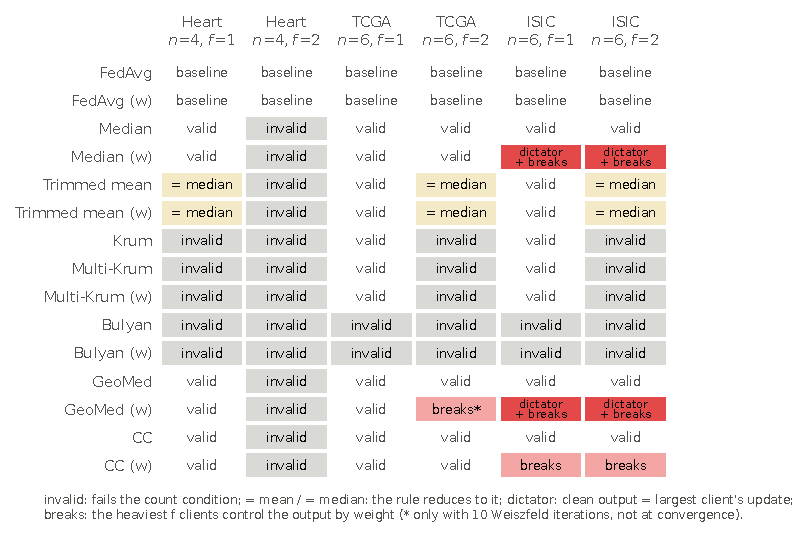
\includegraphics[width=\linewidth]{figures/fig_validity.pdf}
\caption{\texttt{fig\_validity}}
\end{figure}
\begin{figure}[p]\centering
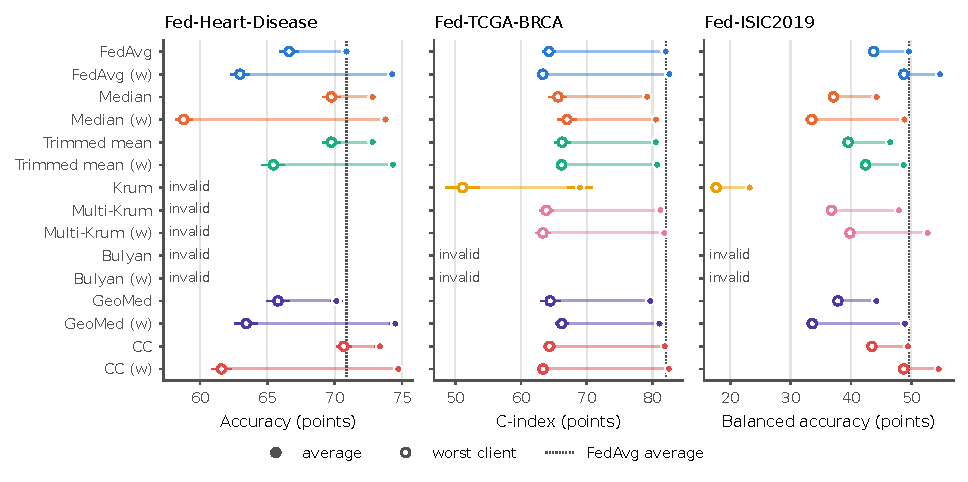
\includegraphics[width=\linewidth]{figures/fig_clean.pdf}
\caption{\texttt{fig\_clean}}
\end{figure}
\begin{figure}[p]\centering
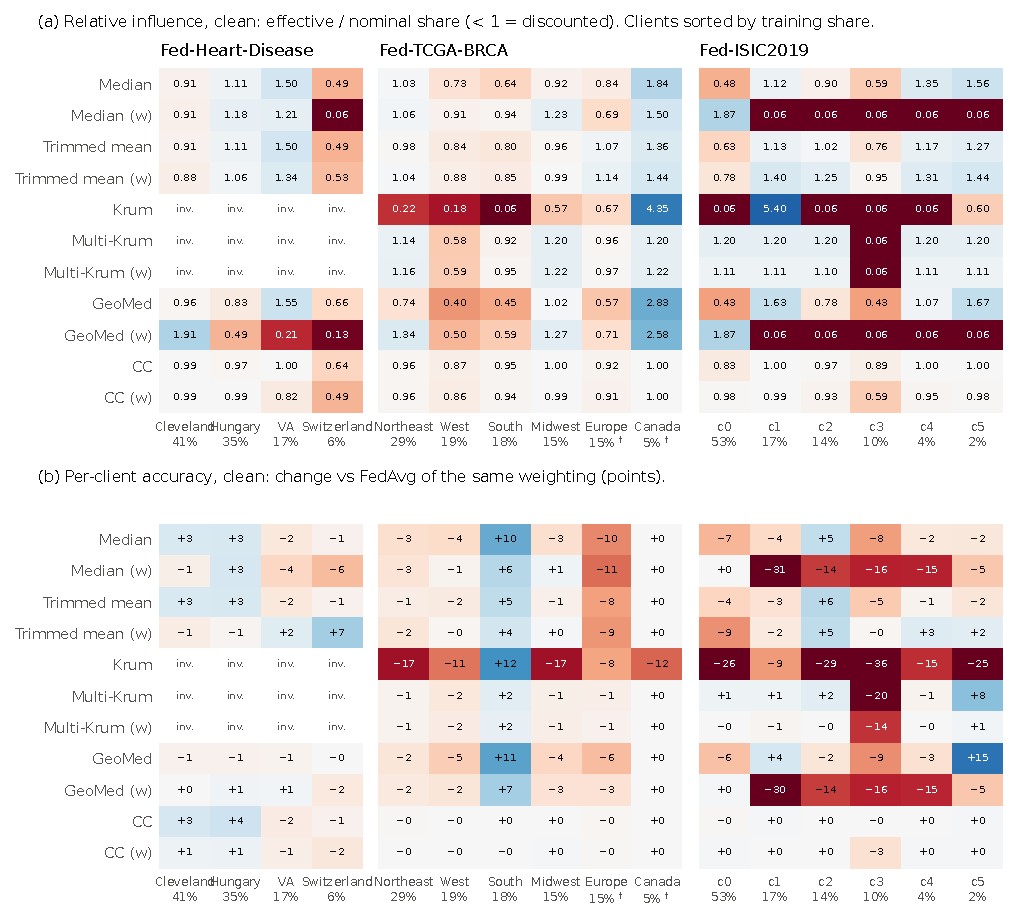
\includegraphics[width=\linewidth]{figures/fig_who_pays.pdf}
\caption{\texttt{fig\_who\_pays}}
\end{figure}
\begin{figure}[p]\centering
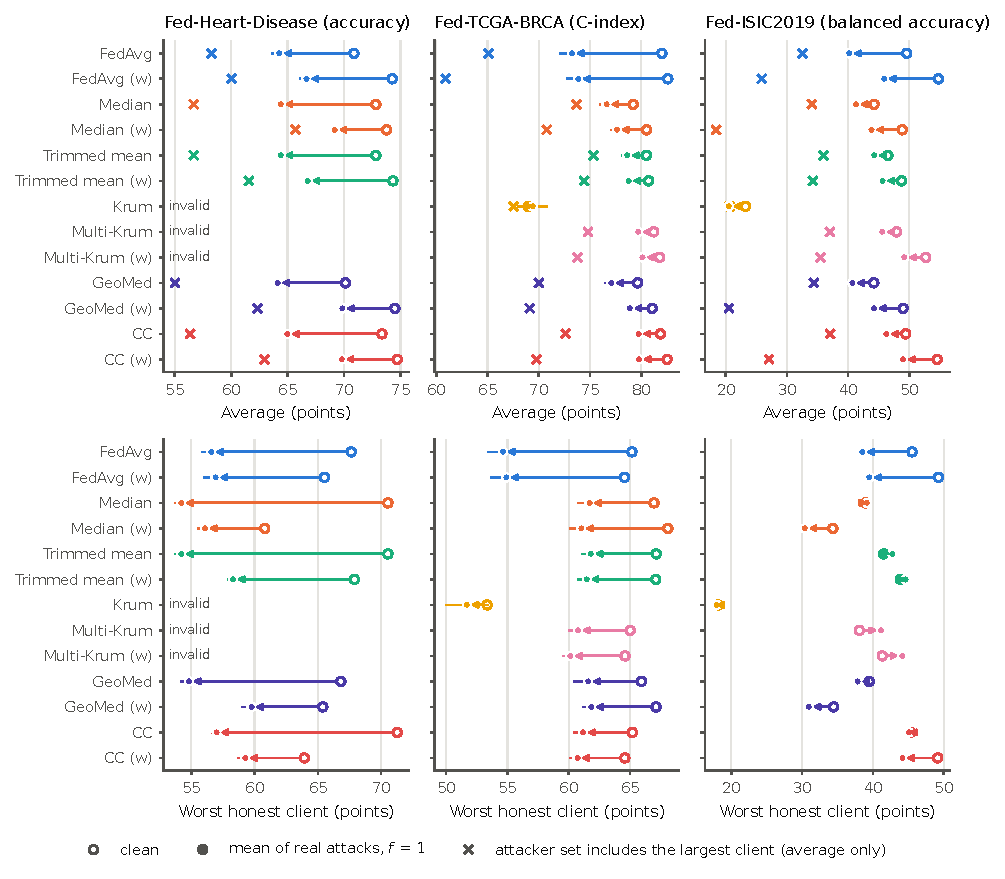
\includegraphics[width=\linewidth]{figures/fig_f1.pdf}
\caption{\texttt{fig\_f1}}
\end{figure}
\begin{figure}[p]\centering
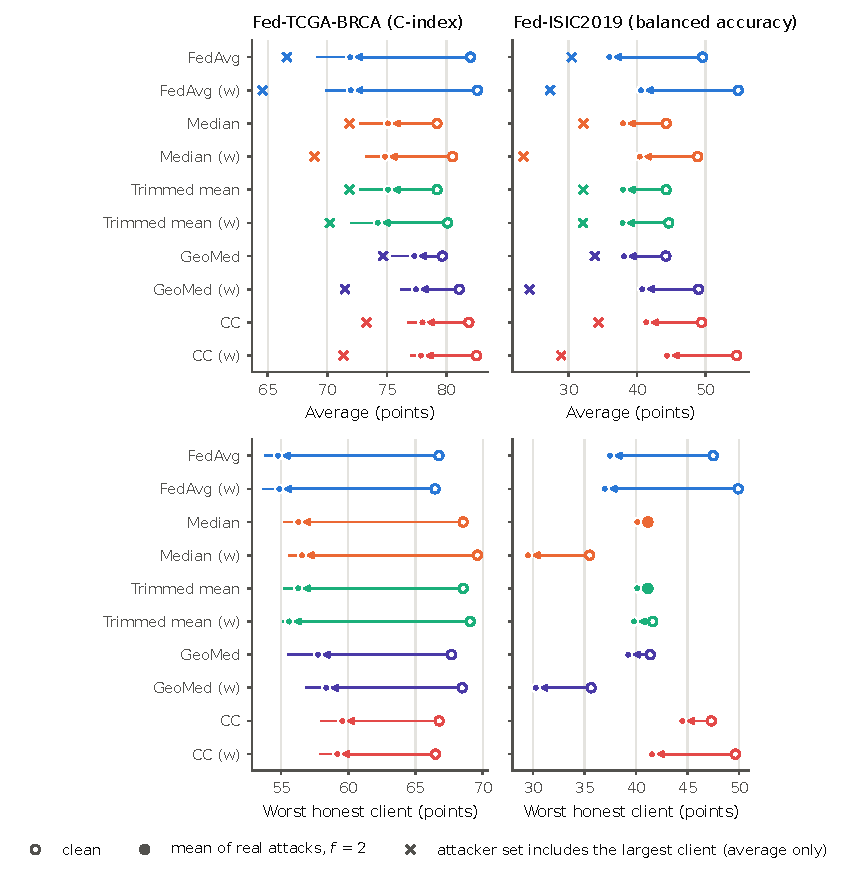
\includegraphics[width=\linewidth]{figures/fig_f2.pdf}
\caption{\texttt{fig\_f2}}
\end{figure}
\begin{figure}[p]\centering
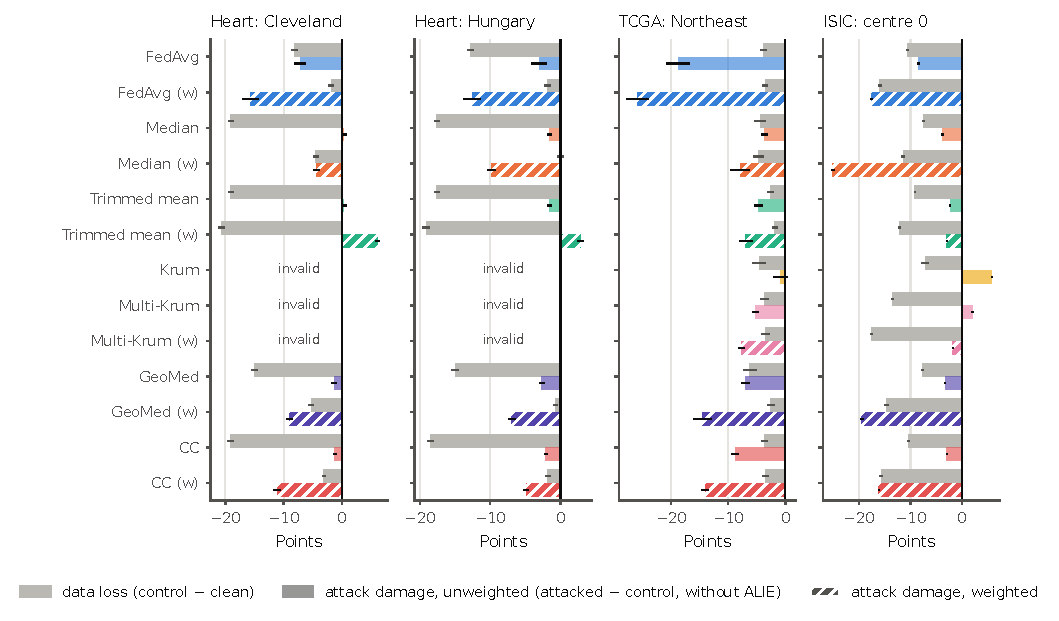
\includegraphics[width=\linewidth]{figures/fig_loo_f1.pdf}
\caption{\texttt{fig\_loo\_f1}}
\end{figure}
\begin{figure}[p]\centering
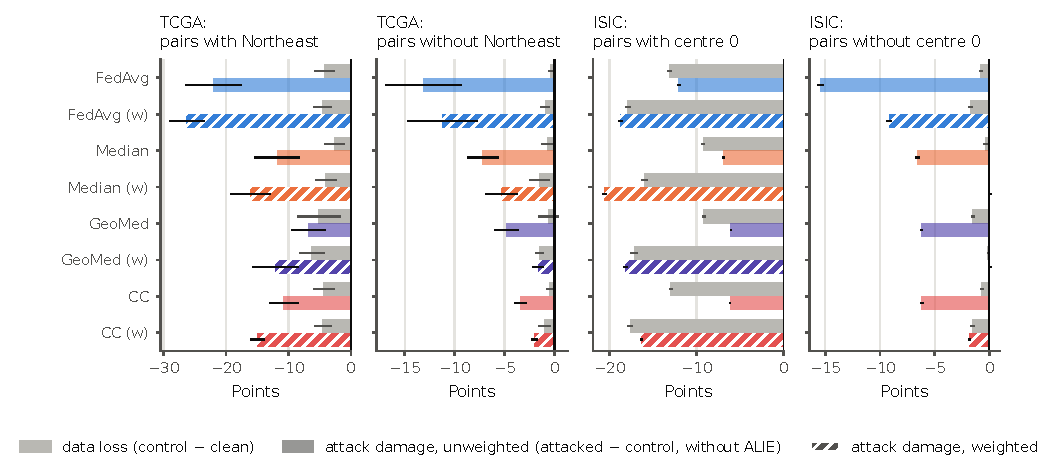
\includegraphics[width=\linewidth]{figures/fig_loo_f2.pdf}
\caption{\texttt{fig\_loo\_f2}}
\end{figure}
\begin{figure}[p]\centering
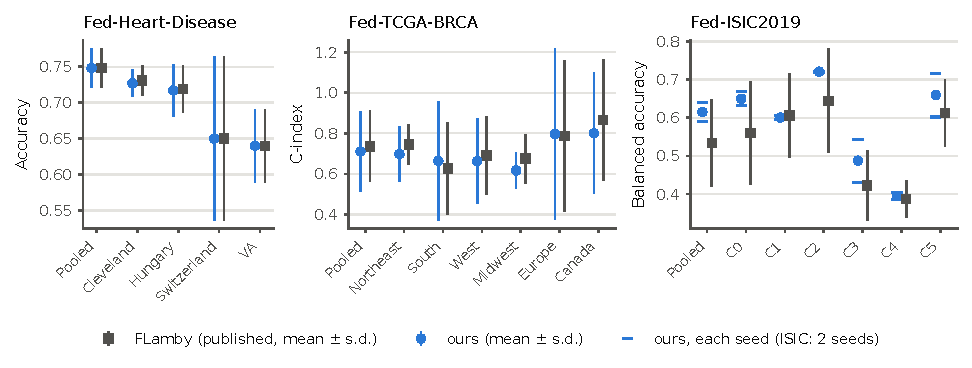
\includegraphics[width=\linewidth]{figures/fig_repro.pdf}
\caption{\texttt{fig\_repro}}
\end{figure}
\begin{table}[p]\centering\small
\caption{\texttt{tab\_settings}}
\resizebox{\linewidth}{!}{% generated by make_paper.py; do not edit by hand
\begin{tabular}{@{}lrp{2.6cm}p{2.6cm}p{2.4cm}rrr@{}}
\toprule
Dataset & $n$ & Training share per client (\%) & Model & Main metric & lr & Rounds & Seeds \\
\midrule
Fed-Heart-Disease & 4 & 41, 35, 6, 17 & logistic regression & accuracy (test-size weighted) & 0.001 & 106 & 20 \\
Fed-TCGA-BRCA & 6 & 29, 18, 19, 15, 15, 5 & linear Cox model & C-index (stratified) & 0.003 & 243 & 20 ($f=2$: 5) \\
Fed-ISIC2019 & 6 & 53, 17, 14, 10, 4, 2 & linear head on frozen EfficientNet-B0 features & balanced accuracy (pooled) & 0.01 & 101 & 20 \\
\bottomrule
\end{tabular}
}
\end{table}
\begin{table}[p]\centering\small
\caption{\texttt{tab\_validity}}
\resizebox{\linewidth}{!}{% generated by make_paper.py; do not edit by hand
\begin{tabular}{@{}l cccc ccc@{}}
\toprule
& \multicolumn{4}{c}{By client count} & \multicolumn{3}{c}{Weighted, by data share} \\
\cmidrule(lr){2-5}\cmidrule(l){6-8}
& \multicolumn{2}{c}{$n=4$ (Heart)} & \multicolumn{2}{c}{$n=6$ (TCGA, ISIC)} & Heart & TCGA & ISIC \\
Rule & $f=1$ & $f=2$ & $f=1$ & $f=2$ & (40.9\%) & (28.6\%) & (53.4\%) \\
\midrule
FedAvg & -- & -- & -- & -- & -- & -- & -- \\
Median & $\checkmark$ & $\times$ & $\checkmark$ & $\checkmark$ & $\checkmark$ & $\checkmark$ & D, B1, B2 \\
Trimmed mean & = median & $\times$ & $\checkmark$ & = median & $\checkmark$ & $\checkmark$ & $\checkmark$ \\
Krum & $\times$ & $\times$ & $\checkmark$ & $\times$ & ignores $w$ & ignores $w$ & ignores $w$ \\
Multi-Krum & $\times$ & $\times$ & $\checkmark$ & $\times$ & n/a & $\checkmark$ & $\checkmark$ \\
Bulyan & $\times$ & $\times$ & $\times$ & $\times$ & n/a & n/a & n/a \\
GeoMed & $\checkmark$ & $\times$ & $\checkmark$ & $\checkmark$ & $\checkmark$ & B2$^*$ & D, B1, B2 \\
CC & $\checkmark$ & $\times$ & $\checkmark$ & $\checkmark$ & $\checkmark$ & $\checkmark$ & B1, B2 \\
\bottomrule
\end{tabular}
}
\end{table}
\begin{table}[p]\centering\small
\caption{\texttt{tab\_clean}}
\resizebox{\linewidth}{!}{% generated by make_paper.py; do not edit by hand
\begin{tabular}{@{}l cccc cccc@{}}
\toprule
& \multicolumn{4}{c}{Unweighted} & \multicolumn{4}{c}{Weighted (w)} \\
\cmidrule(lr){2-5}\cmidrule(l){6-9}
Rule & Avg & Worst & Least influence & $\rho$ & Avg & Worst & Least influence & $\rho$ \\
\midrule
\multicolumn{9}{@{}l}{\textit{Fed-Heart-Disease (accuracy)}} \\
FedAvg & 70.9{\scriptsize\,$\pm$0.4} & 66.6{\scriptsize\,$\pm$0.7} & -- & -- & 74.3{\scriptsize\,$\pm$0.3} & 63.0{\scriptsize\,$\pm$0.7} & -- & -- \\
Median & 72.8{\scriptsize\,$\pm$0.3} & 69.8{\scriptsize\,$\pm$0.6} & Switzerland (0.49) & 0.20 & 73.8{\scriptsize\,$\pm$0.3} & 58.8{\scriptsize\,$\pm$0.6} & Switzerland (0.00) & 0.20 \\
Trimmed mean & 72.8{\scriptsize\,$\pm$0.3} & 69.8{\scriptsize\,$\pm$0.6} & Switzerland (0.49) & 0.20 & 74.3{\scriptsize\,$\pm$0.3} & 65.4{\scriptsize\,$\pm$0.9} & Switzerland (0.53) & 0.20 \\
Krum & invalid &  &  &  & \multicolumn{4}{c}{= Krum (ignores weights)} \\
Multi-Krum & invalid &  &  &  & invalid &  &  &  \\
Bulyan & invalid &  &  &  & invalid &  &  &  \\
GeoMed & 70.1{\scriptsize\,$\pm$0.5} & 65.8{\scriptsize\,$\pm$0.9} & Switzerland (0.66) & 0.40 & 74.5{\scriptsize\,$\pm$0.4} & 63.4{\scriptsize\,$\pm$0.8} & Switzerland (0.13) & 1.00 \\
CC & 73.4{\scriptsize\,$\pm$0.4} & 70.7{\scriptsize\,$\pm$0.6} & Switzerland (0.64) & 0.40 & 74.7{\scriptsize\,$\pm$0.3} & 61.6{\scriptsize\,$\pm$0.7} & Switzerland (0.49) & 1.00 \\
\midrule
\multicolumn{9}{@{}l}{\textit{Fed-TCGA-BRCA (C-index)}} \\
FedAvg & 82.0{\scriptsize\,$\pm$0.4} & 64.3{\scriptsize\,$\pm$0.9} & -- & -- & 82.6{\scriptsize\,$\pm$0.3} & 63.3{\scriptsize\,$\pm$0.7} & -- & -- \\
Median & 79.2{\scriptsize\,$\pm$0.6} & 65.6{\scriptsize\,$\pm$1.4} & South (0.64) & $-$0.35 & 80.5{\scriptsize\,$\pm$0.4} & 67.0{\scriptsize\,$\pm$1.5} & Europe (0.69) & $-$0.38 \\
Trimmed mean & 80.5{\scriptsize\,$\pm$0.4} & 66.3{\scriptsize\,$\pm$1.2} & South (0.80) & $-$0.55 & 80.7{\scriptsize\,$\pm$0.5} & 66.2{\scriptsize\,$\pm$0.7} & South (0.85) & $-$0.55 \\
Krum & 69.0{\scriptsize\,$\pm$1.9} & 51.1{\scriptsize\,$\pm$2.6} & South (0.00) & $-$0.75 & \multicolumn{4}{c}{= Krum (ignores weights)} \\
Multi-Krum & 81.2{\scriptsize\,$\pm$0.3} & 63.8{\scriptsize\,$\pm$1.1} & West (0.58) & $-$0.52 & 81.8{\scriptsize\,$\pm$0.3} & 63.3{\scriptsize\,$\pm$1.1} & West (0.59) & $-$0.52 \\
Bulyan & invalid &  &  &  & invalid &  &  &  \\
GeoMed & 79.7{\scriptsize\,$\pm$0.6} & 64.4{\scriptsize\,$\pm$1.5} & West (0.40) & $-$0.61 & 81.1{\scriptsize\,$\pm$0.3} & 66.2{\scriptsize\,$\pm$1.0} & West (0.50) & $-$0.41 \\
CC & 81.9{\scriptsize\,$\pm$0.3} & 64.3{\scriptsize\,$\pm$1.0} & West (0.87) & $-$0.52 & 82.5{\scriptsize\,$\pm$0.3} & 63.3{\scriptsize\,$\pm$0.8} & West (0.86) & $-$0.52 \\
\midrule
\multicolumn{9}{@{}l}{\textit{Fed-ISIC2019 (balanced accuracy)}} \\
FedAvg & 49.6{\scriptsize\,$\pm$0.2} & 43.8{\scriptsize\,$\pm$0.3} & -- & -- & 54.8{\scriptsize\,$\pm$0.3} & 48.8{\scriptsize\,$\pm$0.4} & -- & -- \\
Median & 44.3{\scriptsize\,$\pm$0.1} & 37.1{\scriptsize\,$\pm$0.2} & c0 (0.48) & $-$0.77 & 48.9{\scriptsize\,$\pm$0.3} & 33.5{\scriptsize\,$\pm$0.9} & c1 (0.00) & 0.66 \\
Trimmed mean & 46.5{\scriptsize\,$\pm$0.1} & 39.5{\scriptsize\,$\pm$0.2} & c0 (0.63) & $-$0.77 & 48.8{\scriptsize\,$\pm$0.2} & 42.4{\scriptsize\,$\pm$0.3} & c0 (0.78) & $-$0.60 \\
Krum & 23.2{\scriptsize\,$\pm$0.7} & 17.7{\scriptsize\,$\pm$0.1} & c0 (0.00) & $-$0.07 & \multicolumn{4}{c}{= Krum (ignores weights)} \\
Multi-Krum & 48.0{\scriptsize\,$\pm$0.2} & 36.8{\scriptsize\,$\pm$0.3} & c3 (0.00) & 0.03 & 52.7{\scriptsize\,$\pm$0.2} & 39.8{\scriptsize\,$\pm$0.6} & c3 (0.00) & 0.03 \\
Bulyan & invalid &  &  &  & invalid &  &  &  \\
GeoMed & 44.2{\scriptsize\,$\pm$0.2} & 37.8{\scriptsize\,$\pm$0.2} & c0 (0.43) & $-$0.60 & 49.0{\scriptsize\,$\pm$0.3} & 33.6{\scriptsize\,$\pm$0.9} & c3 (0.00) & 0.09 \\
CC & 49.4{\scriptsize\,$\pm$0.2} & 43.5{\scriptsize\,$\pm$0.3} & c0 (0.83) & $-$0.71 & 54.6{\scriptsize\,$\pm$0.3} & 48.8{\scriptsize\,$\pm$0.3} & c3 (0.59) & 0.43 \\
\bottomrule
\end{tabular}
}
\end{table}
\begin{table}[p]\centering\small
\caption{\texttt{tab\_f1}}
\resizebox{\linewidth}{!}{% largest client: Cleveland/Northeast/centre 0
% generated by make_paper.py; do not edit by hand
\begin{tabular}{@{}l ccc cc cc@{}}
\toprule
& \multicolumn{3}{c}{Average} & \multicolumn{2}{c}{Worst honest client} & \multicolumn{2}{c}{Largest client attacks: $\Delta$} \\
\cmidrule(lr){2-4}\cmidrule(lr){5-6}\cmidrule(l){7-8}
Rule & Clean & Attacked & $\Delta$ & Clean & Attacked & Avg & Worst \\
\midrule
\multicolumn{8}{@{}l}{\textit{Fed-Heart-Disease, $f=1$}} \\
FedAvg & 70.9{\scriptsize\,$\pm$0.4} & 64.3{\scriptsize\,$\pm$0.7} & $-$6.6 & 67.6{\scriptsize\,$\pm$0.6} & 56.6{\scriptsize\,$\pm$0.7} & $-$12.6{\scriptsize\,$\pm$0.7} & $-$17.5{\scriptsize\,$\pm$1.0} \\
FedAvg (w) & 74.3{\scriptsize\,$\pm$0.3} & 66.7{\scriptsize\,$\pm$0.6} & $-$7.6 & 65.5{\scriptsize\,$\pm$0.8} & 56.9{\scriptsize\,$\pm$1.0} & $-$14.2{\scriptsize\,$\pm$1.1} & $-$12.3{\scriptsize\,$\pm$1.4} \\
Median & 72.8{\scriptsize\,$\pm$0.3} & 64.4{\scriptsize\,$\pm$0.1} & $-$8.4 & 70.5{\scriptsize\,$\pm$0.4} & 54.2{\scriptsize\,$\pm$0.5} & $-$16.1{\scriptsize\,$\pm$0.3} & $-$23.3{\scriptsize\,$\pm$0.9} \\
Median (w) & 73.8{\scriptsize\,$\pm$0.3} & 69.2{\scriptsize\,$\pm$0.2} & $-$4.6 & 60.8{\scriptsize\,$\pm$0.6} & 56.1{\scriptsize\,$\pm$0.6} & $-$8.1{\scriptsize\,$\pm$0.5} & $-$10.3{\scriptsize\,$\pm$1.0} \\
Trimmed mean & 72.8{\scriptsize\,$\pm$0.3} & 64.4{\scriptsize\,$\pm$0.1} & $-$8.4 & 70.5{\scriptsize\,$\pm$0.4} & 54.2{\scriptsize\,$\pm$0.5} & $-$16.1{\scriptsize\,$\pm$0.3} & $-$23.3{\scriptsize\,$\pm$0.9} \\
Trimmed mean (w) & 74.3{\scriptsize\,$\pm$0.3} & 66.8{\scriptsize\,$\pm$0.2} & $-$7.6 & 67.9{\scriptsize\,$\pm$0.7} & 58.3{\scriptsize\,$\pm$0.5} & $-$12.8{\scriptsize\,$\pm$0.4} & $-$13.4{\scriptsize\,$\pm$1.2} \\
GeoMed & 70.1{\scriptsize\,$\pm$0.5} & 64.1{\scriptsize\,$\pm$0.2} & $-$6.0 & 66.8{\scriptsize\,$\pm$0.7} & 54.8{\scriptsize\,$\pm$0.7} & $-$15.1{\scriptsize\,$\pm$0.4} & $-$22.6{\scriptsize\,$\pm$0.8} \\
GeoMed (w) & 74.5{\scriptsize\,$\pm$0.4} & 69.9{\scriptsize\,$\pm$0.3} & $-$4.7 & 65.4{\scriptsize\,$\pm$1.0} & 59.8{\scriptsize\,$\pm$0.8} & $-$12.2{\scriptsize\,$\pm$0.6} & $-$17.2{\scriptsize\,$\pm$1.2} \\
CC & 73.4{\scriptsize\,$\pm$0.4} & 65.0{\scriptsize\,$\pm$0.1} & $-$8.4 & 71.3{\scriptsize\,$\pm$0.5} & 57.0{\scriptsize\,$\pm$0.4} & $-$17.0{\scriptsize\,$\pm$0.4} & $-$25.7{\scriptsize\,$\pm$0.5} \\
CC (w) & 74.7{\scriptsize\,$\pm$0.3} & 69.8{\scriptsize\,$\pm$0.2} & $-$4.9 & 63.9{\scriptsize\,$\pm$0.8} & 59.3{\scriptsize\,$\pm$0.6} & $-$11.7{\scriptsize\,$\pm$0.4} & $-$12.6{\scriptsize\,$\pm$0.5} \\
\midrule
\multicolumn{8}{@{}l}{\textit{Fed-TCGA-BRCA, $f=1$}} \\
FedAvg & 82.0{\scriptsize\,$\pm$0.4} & 73.2{\scriptsize\,$\pm$1.3} & $-$8.8 & 65.2{\scriptsize\,$\pm$0.9} & 54.6{\scriptsize\,$\pm$1.3} & $-$16.9{\scriptsize\,$\pm$1.7} & $-$11.5{\scriptsize\,$\pm$1.8} \\
FedAvg (w) & 82.6{\scriptsize\,$\pm$0.3} & 73.9{\scriptsize\,$\pm$1.1} & $-$8.7 & 64.5{\scriptsize\,$\pm$0.7} & 54.9{\scriptsize\,$\pm$1.3} & $-$21.7{\scriptsize\,$\pm$1.5} & $-$16.1{\scriptsize\,$\pm$1.7} \\
Median & 79.2{\scriptsize\,$\pm$0.6} & 76.6{\scriptsize\,$\pm$0.7} & $-$2.6 & 66.9{\scriptsize\,$\pm$1.2} & 61.7{\scriptsize\,$\pm$1.0} & $-$5.5{\scriptsize\,$\pm$1.0} & $-$7.5{\scriptsize\,$\pm$1.6} \\
Median (w) & 80.5{\scriptsize\,$\pm$0.4} & 77.6{\scriptsize\,$\pm$0.6} & $-$2.9 & 68.1{\scriptsize\,$\pm$1.4} & 61.0{\scriptsize\,$\pm$1.0} & $-$9.7{\scriptsize\,$\pm$1.6} & $-$11.9{\scriptsize\,$\pm$1.7} \\
Trimmed mean & 80.5{\scriptsize\,$\pm$0.4} & 78.6{\scriptsize\,$\pm$0.6} & $-$1.9 & 67.1{\scriptsize\,$\pm$1.1} & 61.8{\scriptsize\,$\pm$0.8} & $-$5.1{\scriptsize\,$\pm$0.9} & $-$7.0{\scriptsize\,$\pm$1.1} \\
Trimmed mean (w) & 80.7{\scriptsize\,$\pm$0.5} & 78.8{\scriptsize\,$\pm$0.5} & $-$2.0 & 67.1{\scriptsize\,$\pm$0.6} & 61.5{\scriptsize\,$\pm$0.8} & $-$6.3{\scriptsize\,$\pm$1.1} & $-$10.1{\scriptsize\,$\pm$1.2} \\
Krum & 69.0{\scriptsize\,$\pm$1.9} & 69.4{\scriptsize\,$\pm$1.5} & +0.5 & 53.3{\scriptsize\,$\pm$2.4} & 51.7{\scriptsize\,$\pm$1.7} & $-$1.4{\scriptsize\,$\pm$0.9} & +0.2{\scriptsize\,$\pm$2.2} \\
Multi-Krum & 81.2{\scriptsize\,$\pm$0.3} & 79.7{\scriptsize\,$\pm$0.4} & $-$1.5 & 65.0{\scriptsize\,$\pm$0.9} & 60.7{\scriptsize\,$\pm$0.8} & $-$6.4{\scriptsize\,$\pm$0.9} & $-$3.7{\scriptsize\,$\pm$1.0} \\
Multi-Krum (w) & 81.8{\scriptsize\,$\pm$0.3} & 80.1{\scriptsize\,$\pm$0.3} & $-$1.7 & 64.6{\scriptsize\,$\pm$1.0} & 60.1{\scriptsize\,$\pm$0.6} & $-$8.0{\scriptsize\,$\pm$0.8} & $-$6.2{\scriptsize\,$\pm$1.2} \\
GeoMed & 79.7{\scriptsize\,$\pm$0.6} & 77.1{\scriptsize\,$\pm$0.7} & $-$2.6 & 65.9{\scriptsize\,$\pm$1.4} & 61.6{\scriptsize\,$\pm$1.2} & $-$9.6{\scriptsize\,$\pm$1.2} & $-$3.4{\scriptsize\,$\pm$1.1} \\
GeoMed (w) & 81.1{\scriptsize\,$\pm$0.3} & 78.9{\scriptsize\,$\pm$0.4} & $-$2.2 & 67.1{\scriptsize\,$\pm$0.9} & 61.8{\scriptsize\,$\pm$0.7} & $-$11.9{\scriptsize\,$\pm$1.6} & $-$10.3{\scriptsize\,$\pm$1.4} \\
CC & 81.9{\scriptsize\,$\pm$0.3} & 79.7{\scriptsize\,$\pm$0.4} & $-$2.1 & 65.2{\scriptsize\,$\pm$0.9} & 61.2{\scriptsize\,$\pm$0.7} & $-$9.3{\scriptsize\,$\pm$0.8} & $-$3.8{\scriptsize\,$\pm$0.9} \\
CC (w) & 82.5{\scriptsize\,$\pm$0.3} & 79.8{\scriptsize\,$\pm$0.3} & $-$2.8 & 64.6{\scriptsize\,$\pm$0.6} & 60.7{\scriptsize\,$\pm$0.6} & $-$12.8{\scriptsize\,$\pm$0.6} & $-$7.5{\scriptsize\,$\pm$1.0} \\
\midrule
\multicolumn{8}{@{}l}{\textit{Fed-ISIC2019, $f=1$}} \\
FedAvg & 49.6{\scriptsize\,$\pm$0.2} & 40.2{\scriptsize\,$\pm$0.1} & $-$9.4 & 45.5{\scriptsize\,$\pm$0.2} & 38.5{\scriptsize\,$\pm$0.2} & $-$17.0{\scriptsize\,$\pm$0.2} & $-$12.3{\scriptsize\,$\pm$0.4} \\
FedAvg (w) & 54.8{\scriptsize\,$\pm$0.3} & 45.9{\scriptsize\,$\pm$0.1} & $-$8.9 & 49.3{\scriptsize\,$\pm$0.3} & 39.5{\scriptsize\,$\pm$0.3} & $-$28.9{\scriptsize\,$\pm$0.3} & $-$30.2{\scriptsize\,$\pm$0.7} \\
Median & 44.3{\scriptsize\,$\pm$0.1} & 41.3{\scriptsize\,$\pm$0.1} & $-$3.0 & 39.0{\scriptsize\,$\pm$0.2} & 39.2{\scriptsize\,$\pm$0.1} & $-$10.2{\scriptsize\,$\pm$0.1} & $-$3.4{\scriptsize\,$\pm$0.3} \\
Median (w) & 48.9{\scriptsize\,$\pm$0.3} & 43.8{\scriptsize\,$\pm$0.2} & $-$5.0 & 34.3{\scriptsize\,$\pm$0.8} & 30.4{\scriptsize\,$\pm$0.6} & $-$30.4{\scriptsize\,$\pm$0.4} & $-$24.3{\scriptsize\,$\pm$0.8} \\
Trimmed mean & 46.5{\scriptsize\,$\pm$0.1} & 44.3{\scriptsize\,$\pm$0.1} & $-$2.2 & 41.5{\scriptsize\,$\pm$0.2} & 42.7{\scriptsize\,$\pm$0.1} & $-$10.5{\scriptsize\,$\pm$0.1} & $-$2.3{\scriptsize\,$\pm$0.3} \\
Trimmed mean (w) & 48.8{\scriptsize\,$\pm$0.2} & 45.6{\scriptsize\,$\pm$0.1} & $-$3.1 & 43.9{\scriptsize\,$\pm$0.2} & 44.6{\scriptsize\,$\pm$0.1} & $-$14.6{\scriptsize\,$\pm$0.2} & $-$4.0{\scriptsize\,$\pm$0.3} \\
Krum & 23.2{\scriptsize\,$\pm$0.7} & 20.5{\scriptsize\,$\pm$0.2} & $-$2.7 & 18.2{\scriptsize\,$\pm$0.1} & 17.9{\scriptsize\,$\pm$0.1} & $-$2.6{\scriptsize\,$\pm$0.7} & $-$0.7{\scriptsize\,$\pm$0.4} \\
Multi-Krum & 48.0{\scriptsize\,$\pm$0.2} & 45.6{\scriptsize\,$\pm$0.1} & $-$2.4 & 38.1{\scriptsize\,$\pm$0.3} & 41.2{\scriptsize\,$\pm$0.1} & $-$10.9{\scriptsize\,$\pm$0.2} & +8.2{\scriptsize\,$\pm$0.3} \\
Multi-Krum (w) & 52.7{\scriptsize\,$\pm$0.2} & 49.2{\scriptsize\,$\pm$0.2} & $-$3.5 & 41.3{\scriptsize\,$\pm$0.5} & 44.1{\scriptsize\,$\pm$0.3} & $-$17.2{\scriptsize\,$\pm$0.2} & +3.2{\scriptsize\,$\pm$0.6} \\
GeoMed & 44.2{\scriptsize\,$\pm$0.2} & 40.7{\scriptsize\,$\pm$0.1} & $-$3.5 & 39.5{\scriptsize\,$\pm$0.2} & 37.8{\scriptsize\,$\pm$0.1} & $-$9.8{\scriptsize\,$\pm$0.2} & $-$5.4{\scriptsize\,$\pm$0.1} \\
GeoMed (w) & 49.0{\scriptsize\,$\pm$0.3} & 44.3{\scriptsize\,$\pm$0.2} & $-$4.7 & 34.5{\scriptsize\,$\pm$0.8} & 31.0{\scriptsize\,$\pm$0.6} & $-$28.5{\scriptsize\,$\pm$0.5} & $-$21.3{\scriptsize\,$\pm$1.0} \\
CC & 49.4{\scriptsize\,$\pm$0.2} & 46.2{\scriptsize\,$\pm$0.1} & $-$3.2 & 45.3{\scriptsize\,$\pm$0.2} & 45.1{\scriptsize\,$\pm$0.1} & $-$12.4{\scriptsize\,$\pm$0.2} & $-$2.3{\scriptsize\,$\pm$0.2} \\
CC (w) & 54.6{\scriptsize\,$\pm$0.3} & 49.0{\scriptsize\,$\pm$0.1} & $-$5.5 & 49.2{\scriptsize\,$\pm$0.3} & 44.2{\scriptsize\,$\pm$0.2} & $-$27.5{\scriptsize\,$\pm$0.3} & $-$26.1{\scriptsize\,$\pm$0.7} \\
\bottomrule
\end{tabular}
}
\end{table}
\begin{table}[p]\centering\small
\caption{\texttt{tab\_f2}}
\resizebox{\linewidth}{!}{% largest client: Northeast/centre 0
% generated by make_paper.py; do not edit by hand
\begin{tabular}{@{}l ccc cc cc@{}}
\toprule
& \multicolumn{3}{c}{Average} & \multicolumn{2}{c}{Worst honest client} & \multicolumn{2}{c}{Largest client attacks: $\Delta$} \\
\cmidrule(lr){2-4}\cmidrule(lr){5-6}\cmidrule(l){7-8}
Rule & Clean & Attacked & $\Delta$ & Clean & Attacked & Avg & Worst \\
\midrule
\multicolumn{8}{@{}l}{\textit{Fed-TCGA-BRCA, $f=2$}} \\
FedAvg & 82.0{\scriptsize\,$\pm$0.4} & 71.9{\scriptsize\,$\pm$2.9} & $-$10.1 & 66.7{\scriptsize\,$\pm$0.8} & 54.8{\scriptsize\,$\pm$1.0} & $-$15.2{\scriptsize\,$\pm$3.8} & $-$16.0{\scriptsize\,$\pm$3.3} \\
FedAvg (w) & 82.6{\scriptsize\,$\pm$0.3} & 72.0{\scriptsize\,$\pm$2.1} & $-$10.6 & 66.5{\scriptsize\,$\pm$0.6} & 54.9{\scriptsize\,$\pm$1.2} & $-$17.9{\scriptsize\,$\pm$2.4} & $-$18.1{\scriptsize\,$\pm$3.5} \\
Median & 79.2{\scriptsize\,$\pm$0.6} & 75.1{\scriptsize\,$\pm$2.4} & $-$4.1 & 68.5{\scriptsize\,$\pm$1.0} & 56.3{\scriptsize\,$\pm$1.1} & $-$7.5{\scriptsize\,$\pm$3.1} & $-$14.8{\scriptsize\,$\pm$3.3} \\
Median (w) & 80.5{\scriptsize\,$\pm$0.4} & 74.8{\scriptsize\,$\pm$1.6} & $-$5.7 & 69.6{\scriptsize\,$\pm$1.2} & 56.6{\scriptsize\,$\pm$1.0} & $-$11.5{\scriptsize\,$\pm$2.5} & $-$20.2{\scriptsize\,$\pm$1.8} \\
Trimmed mean & 79.2{\scriptsize\,$\pm$0.6} & 75.1{\scriptsize\,$\pm$2.4} & $-$4.1 & 68.5{\scriptsize\,$\pm$1.0} & 56.3{\scriptsize\,$\pm$1.1} & $-$7.5{\scriptsize\,$\pm$3.1} & $-$14.8{\scriptsize\,$\pm$3.3} \\
Trimmed mean (w) & 80.1{\scriptsize\,$\pm$0.5} & 74.3{\scriptsize\,$\pm$2.3} & $-$5.8 & 69.1{\scriptsize\,$\pm$1.1} & 55.6{\scriptsize\,$\pm$0.5} & $-$10.1{\scriptsize\,$\pm$3.2} & $-$17.2{\scriptsize\,$\pm$1.1} \\
GeoMed & 79.7{\scriptsize\,$\pm$0.6} & 77.3{\scriptsize\,$\pm$1.9} & $-$2.3 & 67.7{\scriptsize\,$\pm$1.2} & 57.8{\scriptsize\,$\pm$2.3} & $-$5.2{\scriptsize\,$\pm$3.8} & $-$11.9{\scriptsize\,$\pm$4.5} \\
GeoMed (w) & 81.1{\scriptsize\,$\pm$0.3} & 77.5{\scriptsize\,$\pm$1.3} & $-$3.6 & 68.5{\scriptsize\,$\pm$0.8} & 58.4{\scriptsize\,$\pm$1.5} & $-$9.4{\scriptsize\,$\pm$2.9} & $-$16.0{\scriptsize\,$\pm$3.2} \\
CC & 81.9{\scriptsize\,$\pm$0.3} & 78.0{\scriptsize\,$\pm$1.3} & $-$3.9 & 66.8{\scriptsize\,$\pm$0.8} & 59.6{\scriptsize\,$\pm$1.6} & $-$8.4{\scriptsize\,$\pm$2.4} & $-$9.9{\scriptsize\,$\pm$3.2} \\
CC (w) & 82.5{\scriptsize\,$\pm$0.3} & 77.9{\scriptsize\,$\pm$0.9} & $-$4.7 & 66.5{\scriptsize\,$\pm$0.6} & 59.2{\scriptsize\,$\pm$1.3} & $-$11.0{\scriptsize\,$\pm$1.5} & $-$12.5{\scriptsize\,$\pm$2.2} \\
\midrule
\multicolumn{8}{@{}l}{\textit{Fed-ISIC2019, $f=2$}} \\
FedAvg & 49.6{\scriptsize\,$\pm$0.2} & 36.0{\scriptsize\,$\pm$0.1} & $-$13.6 & 47.5{\scriptsize\,$\pm$0.2} & 37.5{\scriptsize\,$\pm$0.1} & $-$19.2{\scriptsize\,$\pm$0.2} & $-$13.6{\scriptsize\,$\pm$0.3} \\
FedAvg (w) & 54.8{\scriptsize\,$\pm$0.3} & 40.6{\scriptsize\,$\pm$0.1} & $-$14.2 & 49.9{\scriptsize\,$\pm$0.3} & 37.0{\scriptsize\,$\pm$0.2} & $-$27.5{\scriptsize\,$\pm$0.3} & $-$25.5{\scriptsize\,$\pm$0.4} \\
Median & 44.3{\scriptsize\,$\pm$0.1} & 37.9{\scriptsize\,$\pm$0.1} & $-$6.3 & 41.2{\scriptsize\,$\pm$0.2} & 40.1{\scriptsize\,$\pm$0.1} & $-$12.1{\scriptsize\,$\pm$0.1} & $-$4.4{\scriptsize\,$\pm$0.3} \\
Median (w) & 48.9{\scriptsize\,$\pm$0.3} & 40.4{\scriptsize\,$\pm$0.2} & $-$8.5 & 35.5{\scriptsize\,$\pm$0.7} & 29.5{\scriptsize\,$\pm$0.4} & $-$25.5{\scriptsize\,$\pm$0.4} & $-$18.0{\scriptsize\,$\pm$0.7} \\
Trimmed mean & 44.3{\scriptsize\,$\pm$0.1} & 37.9{\scriptsize\,$\pm$0.1} & $-$6.3 & 41.2{\scriptsize\,$\pm$0.2} & 40.1{\scriptsize\,$\pm$0.1} & $-$12.1{\scriptsize\,$\pm$0.1} & $-$4.4{\scriptsize\,$\pm$0.3} \\
Trimmed mean (w) & 44.6{\scriptsize\,$\pm$0.1} & 37.9{\scriptsize\,$\pm$0.0} & $-$6.8 & 41.6{\scriptsize\,$\pm$0.2} & 39.8{\scriptsize\,$\pm$0.1} & $-$12.5{\scriptsize\,$\pm$0.1} & $-$5.3{\scriptsize\,$\pm$0.2} \\
GeoMed & 44.2{\scriptsize\,$\pm$0.2} & 38.1{\scriptsize\,$\pm$0.1} & $-$6.1 & 41.4{\scriptsize\,$\pm$0.1} & 39.3{\scriptsize\,$\pm$0.1} & $-$10.4{\scriptsize\,$\pm$0.2} & $-$4.2{\scriptsize\,$\pm$0.1} \\
GeoMed (w) & 49.0{\scriptsize\,$\pm$0.3} & 40.8{\scriptsize\,$\pm$0.2} & $-$8.2 & 35.6{\scriptsize\,$\pm$0.6} & 30.3{\scriptsize\,$\pm$0.4} & $-$24.7{\scriptsize\,$\pm$0.4} & $-$16.6{\scriptsize\,$\pm$0.6} \\
CC & 49.4{\scriptsize\,$\pm$0.2} & 41.4{\scriptsize\,$\pm$0.1} & $-$8.1 & 47.3{\scriptsize\,$\pm$0.2} & 44.5{\scriptsize\,$\pm$0.1} & $-$15.1{\scriptsize\,$\pm$0.2} & $-$5.4{\scriptsize\,$\pm$0.1} \\
CC (w) & 54.6{\scriptsize\,$\pm$0.3} & 44.4{\scriptsize\,$\pm$0.1} & $-$10.2 & 49.6{\scriptsize\,$\pm$0.3} & 41.6{\scriptsize\,$\pm$0.1} & $-$25.7{\scriptsize\,$\pm$0.3} & $-$21.9{\scriptsize\,$\pm$0.4} \\
\bottomrule
\end{tabular}
}
\end{table}
\begin{table}[p]\centering\small
\caption{\texttt{tab\_loo\_f1}}
\resizebox{\linewidth}{!}{% generated by make_paper.py; do not edit by hand
\begin{tabular}{@{}l cc cc cc cc@{}}
\toprule
& \multicolumn{2}{c}{Heart: Cleveland} & \multicolumn{2}{c}{Heart: Hungary} & \multicolumn{2}{c}{TCGA: Northeast} & \multicolumn{2}{c}{ISIC: centre 0} \\
\cmidrule(lr){2-3}\cmidrule(lr){4-5}\cmidrule(lr){6-7}\cmidrule(lr){8-9}
Rule & Data loss & Attack & Data loss & Attack & Data loss & Attack & Data loss & Attack \\
\midrule
FedAvg & $-$8.2{\scriptsize\,$\pm$0.5} & $-$7.2{\scriptsize\,$\pm$1.0} & $-$12.8{\scriptsize\,$\pm$0.4} & $-$3.0{\scriptsize\,$\pm$1.0} & $-$3.8{\scriptsize\,$\pm$0.5} & $-$18.8{\scriptsize\,$\pm$2.1} & $-$10.6{\scriptsize\,$\pm$0.2} & $-$8.5{\scriptsize\,$\pm$0.2} \\
FedAvg (w) & $-$1.9{\scriptsize\,$\pm$0.4} & $-$15.7{\scriptsize\,$\pm$1.4} & $-$1.9{\scriptsize\,$\pm$0.4} & $-$12.6{\scriptsize\,$\pm$1.2} & $-$3.5{\scriptsize\,$\pm$0.4} & $-$25.8{\scriptsize\,$\pm$1.9} & $-$15.9{\scriptsize\,$\pm$0.3} & $-$17.6{\scriptsize\,$\pm$0.2} \\
Median & $-$19.1{\scriptsize\,$\pm$0.4} & +0.3{\scriptsize\,$\pm$0.5} & $-$17.6{\scriptsize\,$\pm$0.4} & $-$1.6{\scriptsize\,$\pm$0.3} & $-$4.4{\scriptsize\,$\pm$1.0} & $-$3.6{\scriptsize\,$\pm$0.6} & $-$7.5{\scriptsize\,$\pm$0.2} & $-$3.8{\scriptsize\,$\pm$0.2} \\
Median (w) & $-$4.5{\scriptsize\,$\pm$0.5} & $-$4.3{\scriptsize\,$\pm$0.5} & +0.0{\scriptsize\,$\pm$0.4} & $-$9.8{\scriptsize\,$\pm$0.6} & $-$4.7{\scriptsize\,$\pm$0.9} & $-$7.9{\scriptsize\,$\pm$1.7} & $-$11.4{\scriptsize\,$\pm$0.4} & $-$25.1{\scriptsize\,$\pm$0.3} \\
Trimmed mean & $-$19.1{\scriptsize\,$\pm$0.4} & +0.3{\scriptsize\,$\pm$0.5} & $-$17.6{\scriptsize\,$\pm$0.4} & $-$1.6{\scriptsize\,$\pm$0.3} & $-$2.6{\scriptsize\,$\pm$0.6} & $-$4.7{\scriptsize\,$\pm$0.7} & $-$9.1{\scriptsize\,$\pm$0.2} & $-$2.3{\scriptsize\,$\pm$0.1} \\
Trimmed mean (w) & $-$20.6{\scriptsize\,$\pm$0.5} & +6.0{\scriptsize\,$\pm$0.4} & $-$19.1{\scriptsize\,$\pm$0.5} & +2.9{\scriptsize\,$\pm$0.4} & $-$1.8{\scriptsize\,$\pm$0.4} & $-$6.9{\scriptsize\,$\pm$1.1} & $-$12.1{\scriptsize\,$\pm$0.2} & $-$3.0{\scriptsize\,$\pm$0.1} \\
Krum & -- & -- & -- & -- & $-$4.5{\scriptsize\,$\pm$1.1} & $-$0.8{\scriptsize\,$\pm$1.2} & $-$7.2{\scriptsize\,$\pm$0.7} & +5.7{\scriptsize\,$\pm$0.1} \\
Multi-Krum & -- & -- & -- & -- & $-$3.6{\scriptsize\,$\pm$0.7} & $-$5.2{\scriptsize\,$\pm$0.5} & $-$13.5{\scriptsize\,$\pm$0.2} & +2.0{\scriptsize\,$\pm$0.1} \\
Multi-Krum (w) & -- & -- & -- & -- & $-$3.5{\scriptsize\,$\pm$0.7} & $-$7.7{\scriptsize\,$\pm$0.5} & $-$17.5{\scriptsize\,$\pm$0.2} & $-$1.7{\scriptsize\,$\pm$0.1} \\
GeoMed & $-$15.0{\scriptsize\,$\pm$0.5} & $-$1.4{\scriptsize\,$\pm$0.4} & $-$15.0{\scriptsize\,$\pm$0.5} & $-$2.6{\scriptsize\,$\pm$0.4} & $-$6.2{\scriptsize\,$\pm$1.2} & $-$6.9{\scriptsize\,$\pm$0.7} & $-$7.7{\scriptsize\,$\pm$0.2} & $-$3.3{\scriptsize\,$\pm$0.1} \\
GeoMed (w) & $-$5.3{\scriptsize\,$\pm$0.4} & $-$9.0{\scriptsize\,$\pm$0.5} & $-$0.7{\scriptsize\,$\pm$0.3} & $-$6.9{\scriptsize\,$\pm$0.5} & $-$2.5{\scriptsize\,$\pm$0.6} & $-$14.5{\scriptsize\,$\pm$1.6} & $-$14.6{\scriptsize\,$\pm$0.4} & $-$19.5{\scriptsize\,$\pm$0.3} \\
CC & $-$19.0{\scriptsize\,$\pm$0.5} & $-$1.2{\scriptsize\,$\pm$0.2} & $-$18.5{\scriptsize\,$\pm$0.4} & $-$2.1{\scriptsize\,$\pm$0.2} & $-$3.7{\scriptsize\,$\pm$0.5} & $-$8.7{\scriptsize\,$\pm$0.6} & $-$10.4{\scriptsize\,$\pm$0.2} & $-$2.9{\scriptsize\,$\pm$0.1} \\
CC (w) & $-$3.1{\scriptsize\,$\pm$0.3} & $-$11.1{\scriptsize\,$\pm$0.6} & $-$1.8{\scriptsize\,$\pm$0.4} & $-$4.8{\scriptsize\,$\pm$0.4} & $-$3.5{\scriptsize\,$\pm$0.5} & $-$14.1{\scriptsize\,$\pm$0.5} & $-$15.6{\scriptsize\,$\pm$0.3} & $-$16.1{\scriptsize\,$\pm$0.1} \\
\bottomrule
\end{tabular}
}
\end{table}
\begin{table}[p]\centering\small
\caption{\texttt{tab\_loo\_f2}}
\resizebox{\linewidth}{!}{% generated by make_paper.py; do not edit by hand
\begin{tabular}{@{}l cc cc cc cc@{}}
\toprule
& \multicolumn{2}{c}{TCGA: with Northeast (pairs)} & \multicolumn{2}{c}{TCGA: without Northeast (pairs)} & \multicolumn{2}{c}{ISIC: with centre 0 (pairs)} & \multicolumn{2}{c}{ISIC: without centre 0 (pairs)} \\
\cmidrule(lr){2-3}\cmidrule(lr){4-5}\cmidrule(lr){6-7}\cmidrule(lr){8-9}
Rule & Data loss & Attack & Data loss & Attack & Data loss & Attack & Data loss & Attack \\
\midrule
FedAvg & $-$4.3{\scriptsize\,$\pm$1.6} & $-$22.0{\scriptsize\,$\pm$4.5} & $-$0.4{\scriptsize\,$\pm$0.2} & $-$13.1{\scriptsize\,$\pm$3.8} & $-$13.1{\scriptsize\,$\pm$0.2} & $-$12.0{\scriptsize\,$\pm$0.1} & $-$0.8{\scriptsize\,$\pm$0.2} & $-$15.4{\scriptsize\,$\pm$0.2} \\
FedAvg (w) & $-$4.5{\scriptsize\,$\pm$1.5} & $-$26.3{\scriptsize\,$\pm$2.8} & $-$0.9{\scriptsize\,$\pm$0.5} & $-$11.2{\scriptsize\,$\pm$3.5} & $-$17.9{\scriptsize\,$\pm$0.3} & $-$18.7{\scriptsize\,$\pm$0.2} & $-$1.7{\scriptsize\,$\pm$0.2} & $-$9.2{\scriptsize\,$\pm$0.2} \\
Median & $-$2.7{\scriptsize\,$\pm$1.6} & $-$11.8{\scriptsize\,$\pm$3.6} & $-$0.7{\scriptsize\,$\pm$0.6} & $-$7.2{\scriptsize\,$\pm$1.6} & $-$9.3{\scriptsize\,$\pm$0.1} & $-$6.9{\scriptsize\,$\pm$0.1} & $-$0.3{\scriptsize\,$\pm$0.2} & $-$6.6{\scriptsize\,$\pm$0.2} \\
Median (w) & $-$4.0{\scriptsize\,$\pm$1.7} & $-$16.1{\scriptsize\,$\pm$3.2} & $-$1.5{\scriptsize\,$\pm$1.0} & $-$5.3{\scriptsize\,$\pm$1.6} & $-$16.0{\scriptsize\,$\pm$0.3} & $-$20.6{\scriptsize\,$\pm$0.3} & +0.0{\scriptsize\,$\pm$0.0} & +0.0{\scriptsize\,$\pm$0.1} \\
GeoMed & $-$5.2{\scriptsize\,$\pm$3.4} & $-$6.8{\scriptsize\,$\pm$2.7} & $-$0.6{\scriptsize\,$\pm$1.0} & $-$4.8{\scriptsize\,$\pm$1.2} & $-$9.2{\scriptsize\,$\pm$0.2} & $-$6.1{\scriptsize\,$\pm$0.1} & $-$1.5{\scriptsize\,$\pm$0.2} & $-$6.2{\scriptsize\,$\pm$0.1} \\
GeoMed (w) & $-$6.2{\scriptsize\,$\pm$2.0} & $-$12.0{\scriptsize\,$\pm$3.7} & $-$1.5{\scriptsize\,$\pm$0.4} & $-$1.6{\scriptsize\,$\pm$0.6} & $-$17.2{\scriptsize\,$\pm$0.4} & $-$18.2{\scriptsize\,$\pm$0.2} & $-$0.1{\scriptsize\,$\pm$0.0} & +0.1{\scriptsize\,$\pm$0.1} \\
CC & $-$4.4{\scriptsize\,$\pm$1.7} & $-$10.8{\scriptsize\,$\pm$2.3} & $-$0.5{\scriptsize\,$\pm$0.3} & $-$3.4{\scriptsize\,$\pm$0.6} & $-$12.9{\scriptsize\,$\pm$0.2} & $-$6.2{\scriptsize\,$\pm$0.1} & $-$0.7{\scriptsize\,$\pm$0.2} & $-$6.2{\scriptsize\,$\pm$0.1} \\
CC (w) & $-$4.5{\scriptsize\,$\pm$1.4} & $-$15.0{\scriptsize\,$\pm$1.2} & $-$1.0{\scriptsize\,$\pm$0.6} & $-$2.0{\scriptsize\,$\pm$0.3} & $-$17.6{\scriptsize\,$\pm$0.3} & $-$16.4{\scriptsize\,$\pm$0.1} & $-$1.6{\scriptsize\,$\pm$0.2} & $-$1.8{\scriptsize\,$\pm$0.1} \\
\bottomrule
\end{tabular}
}
\end{table}
\begin{table}[p]\centering\small
\caption{\texttt{tab\_repro}}
\resizebox{\linewidth}{!}{% generated by make_paper.py; do not edit by hand
\begin{tabular}{@{}l l l r c@{}}
\toprule
Test set & Ours & FLamby (published) & Difference & Within 1 s.d. \\
\midrule
\multicolumn{5}{@{}l}{\textit{Fed-Heart-Disease, accuracy, 5 seeds}} \\
Pooled & 0.748 $\pm$ 0.027 & 0.748 $\pm$ 0.027 & +0.000 & yes \\
Cleveland & 0.727 $\pm$ 0.019 & 0.731 $\pm$ 0.022 & $-$0.004 & yes \\
Hungary & 0.717 $\pm$ 0.037 & 0.719 $\pm$ 0.033 & $-$0.002 & yes \\
Switzerland & 0.650 $\pm$ 0.114 & 0.650 $\pm$ 0.114 & +0.000 & yes \\
Va & 0.640 $\pm$ 0.051 & 0.640 $\pm$ 0.051 & +0.000 & yes \\
\midrule
\multicolumn{5}{@{}l}{\textit{Fed-TCGA-BRCA, C-index, 5 seeds}} \\
Pooled & 0.710 $\pm$ 0.196 & 0.735 $\pm$ 0.175 & $-$0.025 & yes \\
Northeast & 0.698 $\pm$ 0.134 & 0.745 $\pm$ 0.099 & $-$0.047 & yes \\
South & 0.664 $\pm$ 0.292 & 0.627 $\pm$ 0.228 & +0.036 & yes \\
West & 0.663 $\pm$ 0.211 & 0.691 $\pm$ 0.190 & $-$0.028 & yes \\
Midwest & 0.617 $\pm$ 0.089 & 0.675 $\pm$ 0.120 & $-$0.058 & yes \\
Europe & 0.796 $\pm$ 0.421 & 0.787 $\pm$ 0.373 & +0.009 & yes \\
Canada & 0.800 $\pm$ 0.298 & 0.867 $\pm$ 0.298 & $-$0.067 & yes \\
\midrule
\multicolumn{5}{@{}l}{\textit{Fed-ISIC2019, balanced accuracy, FLamby's code, 2 seeds (ours) vs 5}} \\
Pooled & 0.615 (0.639, 0.591) & 0.534 $\pm$ 0.114 & +0.081 & yes \\
Centre 0 & 0.650 (0.668, 0.632) & 0.560 $\pm$ 0.136 & +0.090 & yes \\
Centre 1 & 0.601 (0.605, 0.596) & 0.606 $\pm$ 0.110 & $-$0.005 & yes \\
Centre 2 & 0.721 (0.722, 0.720) & 0.645 $\pm$ 0.136 & +0.076 & yes \\
Centre 3 & 0.488 (0.544, 0.431) & 0.423 $\pm$ 0.091 & +0.065 & yes \\
Centre 4 & 0.396 (0.386, 0.405) & 0.387 $\pm$ 0.049 & +0.009 & yes \\
Centre 5 & 0.660 (0.717, 0.602) & 0.612 $\pm$ 0.088 & +0.047 & yes \\
\bottomrule
\end{tabular}
}
\end{table}
\begin{table}[p]\centering\small
\caption{\texttt{tab\_influence\_heart}}
\resizebox{\linewidth}{!}{% generated by make_paper.py; do not edit by hand
\begin{tabular}{@{}lrrrr@{}}
\toprule
Rule & Cleveland & Hungary & VA & Switzerland \\
\midrule
Median & 0.91 & 1.11 & 1.50 & 0.49 \\
Median (w) & 0.91 & 1.18 & 1.21 & 0.00 \\
Trimmed mean & 0.91 & 1.11 & 1.50 & 0.49 \\
Trimmed mean (w) & 0.88 & 1.06 & 1.34 & 0.53 \\
GeoMed & 0.96 & 0.83 & 1.55 & 0.66 \\
GeoMed (w) & 1.91 & 0.49 & 0.21 & 0.13 \\
CC & 0.99 & 0.97 & 1.00 & 0.64 \\
CC (w) & 0.99 & 0.99 & 0.82 & 0.49 \\
\bottomrule
\end{tabular}
}
\end{table}
\begin{table}[p]\centering\small
\caption{\texttt{tab\_influence\_tcga}}
\resizebox{\linewidth}{!}{% generated by make_paper.py; do not edit by hand
\begin{tabular}{@{}lrrrrrr@{}}
\toprule
Rule & Northeast & South & West & Midwest & Europe & Canada \\
\midrule
Median & 1.03 & 0.64 & 0.73 & 0.92 & 0.84 & 1.84 \\
Median (w) & 1.06 & 0.94 & 0.91 & 1.23 & 0.69 & 1.50 \\
Trimmed mean & 0.98 & 0.80 & 0.84 & 0.96 & 1.07 & 1.36 \\
Trimmed mean (w) & 1.04 & 0.85 & 0.88 & 0.99 & 1.14 & 1.44 \\
Krum & 0.22 & 0.00 & 0.18 & 0.57 & 0.67 & 4.35 \\
Multi-Krum & 1.14 & 0.92 & 0.58 & 1.20 & 0.96 & 1.20 \\
Multi-Krum (w) & 1.16 & 0.95 & 0.59 & 1.22 & 0.97 & 1.22 \\
GeoMed & 0.74 & 0.45 & 0.40 & 1.02 & 0.57 & 2.83 \\
GeoMed (w) & 1.34 & 0.59 & 0.50 & 1.27 & 0.71 & 2.58 \\
CC & 0.96 & 0.95 & 0.87 & 1.00 & 0.92 & 1.00 \\
CC (w) & 0.96 & 0.94 & 0.86 & 0.99 & 0.91 & 1.00 \\
\bottomrule
\end{tabular}
}
\end{table}
\begin{table}[p]\centering\small
\caption{\texttt{tab\_influence\_isic}}
\resizebox{\linewidth}{!}{% generated by make_paper.py; do not edit by hand
\begin{tabular}{@{}lrrrrrr@{}}
\toprule
Rule & Centre 0 & Centre 1 & Centre 2 & Centre 3 & Centre 4 & Centre 5 \\
\midrule
Median & 0.48 & 1.12 & 0.90 & 0.59 & 1.35 & 1.56 \\
Median (w) & 1.87 & 0.00 & 0.00 & 0.00 & 0.00 & 0.00 \\
Trimmed mean & 0.63 & 1.13 & 1.02 & 0.76 & 1.17 & 1.27 \\
Trimmed mean (w) & 0.78 & 1.40 & 1.25 & 0.95 & 1.31 & 1.44 \\
Krum & 0.00 & 5.40 & 0.00 & 0.00 & 0.00 & 0.60 \\
Multi-Krum & 1.20 & 1.20 & 1.20 & 0.00 & 1.20 & 1.20 \\
Multi-Krum (w) & 1.11 & 1.11 & 1.10 & 0.00 & 1.11 & 1.11 \\
GeoMed & 0.43 & 1.63 & 0.78 & 0.43 & 1.07 & 1.67 \\
GeoMed (w) & 1.87 & 0.01 & 0.00 & 0.00 & 0.01 & 0.01 \\
CC & 0.83 & 1.00 & 0.97 & 0.89 & 1.00 & 1.00 \\
CC (w) & 0.98 & 0.99 & 0.93 & 0.59 & 0.95 & 0.98 \\
\bottomrule
\end{tabular}
}
\end{table}
\begin{table}[p]\centering\small
\caption{\texttt{tab\_loo\_heart\_f1\_all}}
\resizebox{\linewidth}{!}{% generated by make_paper.py; do not edit by hand
\begin{tabular}{@{}l ccc cc@{}}
\toprule
& \multicolumn{3}{c}{Average} & \multicolumn{2}{c}{Worst honest client} \\
\cmidrule(lr){2-4}\cmidrule(l){5-6}
Rule & Data loss & Attack (no ALIE) & Attack (all) & Data loss & Attack (no ALIE) \\
\midrule
\multicolumn{6}{@{}l}{\textit{Left out / attacking: Cleveland}} \\
FedAvg & $-$8.2{\scriptsize\,$\pm$0.5} & $-$7.2{\scriptsize\,$\pm$1.0} & $-$4.4{\scriptsize\,$\pm$0.8} & $-$15.2{\scriptsize\,$\pm$0.8} & $-$6.5{\scriptsize\,$\pm$1.1} \\
FedAvg (w) & $-$1.9{\scriptsize\,$\pm$0.4} & $-$15.7{\scriptsize\,$\pm$1.4} & $-$12.3{\scriptsize\,$\pm$1.2} & $-$0.5{\scriptsize\,$\pm$0.8} & $-$12.9{\scriptsize\,$\pm$1.8} \\
Median & $-$19.1{\scriptsize\,$\pm$0.4} & +0.3{\scriptsize\,$\pm$0.5} & +2.9{\scriptsize\,$\pm$0.4} & $-$29.2{\scriptsize\,$\pm$0.9} & +1.0{\scriptsize\,$\pm$0.6} \\
Median (w)$^\ddagger$ & $-$4.5{\scriptsize\,$\pm$0.5} & $-$4.3{\scriptsize\,$\pm$0.5} & $-$3.6{\scriptsize\,$\pm$0.4} & $-$9.3{\scriptsize\,$\pm$0.8} & +2.0{\scriptsize\,$\pm$1.2} \\
Trimmed mean & $-$19.1{\scriptsize\,$\pm$0.4} & +0.3{\scriptsize\,$\pm$0.5} & +2.9{\scriptsize\,$\pm$0.4} & $-$29.2{\scriptsize\,$\pm$0.9} & +1.0{\scriptsize\,$\pm$0.6} \\
Trimmed mean (w) & $-$20.6{\scriptsize\,$\pm$0.5} & +6.0{\scriptsize\,$\pm$0.4} & +7.8{\scriptsize\,$\pm$0.4} & $-$24.9{\scriptsize\,$\pm$1.1} & +10.4{\scriptsize\,$\pm$1.0} \\
GeoMed & $-$15.0{\scriptsize\,$\pm$0.5} & $-$1.4{\scriptsize\,$\pm$0.5} & $-$0.1{\scriptsize\,$\pm$0.4} & $-$21.3{\scriptsize\,$\pm$0.9} & $-$2.3{\scriptsize\,$\pm$0.6} \\
GeoMed (w)$^\ddagger$ & $-$5.3{\scriptsize\,$\pm$0.5} & $-$9.0{\scriptsize\,$\pm$0.5} & $-$6.9{\scriptsize\,$\pm$0.4} & $-$13.8{\scriptsize\,$\pm$0.9} & $-$2.0{\scriptsize\,$\pm$1.1} \\
CC & $-$19.0{\scriptsize\,$\pm$0.5} & $-$1.2{\scriptsize\,$\pm$0.2} & +2.0{\scriptsize\,$\pm$0.2} & $-$31.1{\scriptsize\,$\pm$0.6} & $-$0.2{\scriptsize\,$\pm$0.4} \\
CC (w) & $-$3.1{\scriptsize\,$\pm$0.3} & $-$11.1{\scriptsize\,$\pm$0.6} & $-$8.6{\scriptsize\,$\pm$0.5} & $-$2.0{\scriptsize\,$\pm$0.7} & $-$11.0{\scriptsize\,$\pm$1.1} \\
\multicolumn{6}{@{}l}{\textit{Left out / attacking: Hungary}} \\
FedAvg & $-$12.8{\scriptsize\,$\pm$0.4} & $-$3.0{\scriptsize\,$\pm$1.0} & $-$0.7{\scriptsize\,$\pm$0.8} & $-$12.9{\scriptsize\,$\pm$0.5} & $-$7.7{\scriptsize\,$\pm$1.2} \\
FedAvg (w) & $-$1.9{\scriptsize\,$\pm$0.4} & $-$12.6{\scriptsize\,$\pm$1.2} & $-$9.6{\scriptsize\,$\pm$0.9} & +7.7{\scriptsize\,$\pm$1.2} & $-$16.1{\scriptsize\,$\pm$1.6} \\
Median & $-$17.6{\scriptsize\,$\pm$0.4} & $-$1.6{\scriptsize\,$\pm$0.3} & +0.9{\scriptsize\,$\pm$0.3} & $-$19.3{\scriptsize\,$\pm$0.4} & $-$2.9{\scriptsize\,$\pm$0.5} \\
Median (w)$^\ddagger$ & +0.0{\scriptsize\,$\pm$0.4} & $-$9.8{\scriptsize\,$\pm$0.6} & $-$7.9{\scriptsize\,$\pm$0.5} & +6.7{\scriptsize\,$\pm$0.9} & $-$5.1{\scriptsize\,$\pm$0.9} \\
Trimmed mean & $-$17.6{\scriptsize\,$\pm$0.4} & $-$1.6{\scriptsize\,$\pm$0.3} & +0.9{\scriptsize\,$\pm$0.3} & $-$19.3{\scriptsize\,$\pm$0.4} & $-$2.9{\scriptsize\,$\pm$0.5} \\
Trimmed mean (w) & $-$19.1{\scriptsize\,$\pm$0.5} & +2.9{\scriptsize\,$\pm$0.4} & +5.6{\scriptsize\,$\pm$0.4} & $-$11.9{\scriptsize\,$\pm$1.1} & +3.6{\scriptsize\,$\pm$0.7} \\
GeoMed & $-$15.0{\scriptsize\,$\pm$0.5} & $-$2.6{\scriptsize\,$\pm$0.4} & $-$1.1{\scriptsize\,$\pm$0.3} & $-$18.0{\scriptsize\,$\pm$0.8} & $-$3.5{\scriptsize\,$\pm$0.6} \\
GeoMed (w)$^\ddagger$ & $-$0.7{\scriptsize\,$\pm$0.3} & $-$6.9{\scriptsize\,$\pm$0.5} & $-$5.4{\scriptsize\,$\pm$0.4} & +2.1{\scriptsize\,$\pm$0.8} & $-$2.2{\scriptsize\,$\pm$1.0} \\
CC & $-$18.5{\scriptsize\,$\pm$0.4} & $-$2.1{\scriptsize\,$\pm$0.2} & +1.3{\scriptsize\,$\pm$0.2} & $-$20.0{\scriptsize\,$\pm$0.9} & $-$4.2{\scriptsize\,$\pm$0.3} \\
CC (w) & $-$1.8{\scriptsize\,$\pm$0.4} & $-$4.8{\scriptsize\,$\pm$0.4} & $-$3.5{\scriptsize\,$\pm$0.3} & +9.3{\scriptsize\,$\pm$0.9} & $-$4.6{\scriptsize\,$\pm$0.6} \\
\multicolumn{6}{@{}l}{\textit{Left out / attacking: Switzerland}} \\
FedAvg & +2.3{\scriptsize\,$\pm$0.4} & $-$4.2{\scriptsize\,$\pm$0.9} & $-$3.0{\scriptsize\,$\pm$0.8} & $-$2.9{\scriptsize\,$\pm$1.0} & $-$10.8{\scriptsize\,$\pm$1.0} \\
FedAvg (w) & +0.4{\scriptsize\,$\pm$0.3} & $-$1.6{\scriptsize\,$\pm$0.4} & $-$1.2{\scriptsize\,$\pm$0.4} & $-$1.7{\scriptsize\,$\pm$0.7} & $-$2.4{\scriptsize\,$\pm$0.8} \\
Median & +1.0{\scriptsize\,$\pm$0.5} & $-$0.7{\scriptsize\,$\pm$0.3} & $-$0.4{\scriptsize\,$\pm$0.3} & $-$11.0{\scriptsize\,$\pm$0.7} & $-$3.0{\scriptsize\,$\pm$0.6} \\
Median (w) & +0.0{\scriptsize\,$\pm$0.0} & +0.0{\scriptsize\,$\pm$0.0} & +0.0{\scriptsize\,$\pm$0.0} & +0.0{\scriptsize\,$\pm$0.0} & $-$0.0{\scriptsize\,$\pm$0.1} \\
Trimmed mean & +1.0{\scriptsize\,$\pm$0.5} & $-$0.7{\scriptsize\,$\pm$0.3} & $-$0.4{\scriptsize\,$\pm$0.3} & $-$11.0{\scriptsize\,$\pm$0.7} & $-$3.0{\scriptsize\,$\pm$0.6} \\
Trimmed mean (w) & $-$0.6{\scriptsize\,$\pm$0.3} & $-$0.4{\scriptsize\,$\pm$0.3} & $-$0.5{\scriptsize\,$\pm$0.3} & $-$6.7{\scriptsize\,$\pm$0.8} & $-$2.2{\scriptsize\,$\pm$0.6} \\
GeoMed & +4.7{\scriptsize\,$\pm$0.6} & $-$1.2{\scriptsize\,$\pm$0.3} & $-$1.1{\scriptsize\,$\pm$0.3} & $-$5.5{\scriptsize\,$\pm$1.2} & $-$3.6{\scriptsize\,$\pm$0.7} \\
GeoMed (w) & +0.1{\scriptsize\,$\pm$0.2} & $-$0.1{\scriptsize\,$\pm$0.2} & $-$0.1{\scriptsize\,$\pm$0.2} & $-$0.0{\scriptsize\,$\pm$0.1} & $-$1.3{\scriptsize\,$\pm$0.5} \\
CC & $-$0.1{\scriptsize\,$\pm$0.5} & +0.2{\scriptsize\,$\pm$0.2} & +0.5{\scriptsize\,$\pm$0.3} & $-$7.3{\scriptsize\,$\pm$1.1} & $-$5.1{\scriptsize\,$\pm$0.6} \\
CC (w) & $-$0.1{\scriptsize\,$\pm$0.3} & $-$0.3{\scriptsize\,$\pm$0.3} & $-$0.3{\scriptsize\,$\pm$0.3} & $-$1.6{\scriptsize\,$\pm$0.5} & $-$1.1{\scriptsize\,$\pm$0.5} \\
\multicolumn{6}{@{}l}{\textit{Left out / attacking: VA}} \\
FedAvg & +3.2{\scriptsize\,$\pm$0.6} & $-$3.8{\scriptsize\,$\pm$1.0} & $-$2.8{\scriptsize\,$\pm$0.9} & +6.1{\scriptsize\,$\pm$1.0} & $-$4.9{\scriptsize\,$\pm$1.0} \\
FedAvg (w) & $-$0.6{\scriptsize\,$\pm$0.3} & $-$4.0{\scriptsize\,$\pm$0.7} & $-$3.3{\scriptsize\,$\pm$0.6} & $-$3.2{\scriptsize\,$\pm$1.5} & $-$10.6{\scriptsize\,$\pm$1.5} \\
Median & $-$0.5{\scriptsize\,$\pm$0.4} & $-$1.0{\scriptsize\,$\pm$0.4} & $-$1.0{\scriptsize\,$\pm$0.3} & +1.9{\scriptsize\,$\pm$1.6} & $-$9.5{\scriptsize\,$\pm$1.2} \\
Median (w) & $-$1.4{\scriptsize\,$\pm$0.6} & $-$1.1{\scriptsize\,$\pm$0.4} & $-$1.0{\scriptsize\,$\pm$0.4} & +4.8{\scriptsize\,$\pm$1.5} & $-$12.6{\scriptsize\,$\pm$1.4} \\
Trimmed mean & $-$0.5{\scriptsize\,$\pm$0.4} & $-$1.0{\scriptsize\,$\pm$0.4} & $-$1.0{\scriptsize\,$\pm$0.3} & +1.9{\scriptsize\,$\pm$1.6} & $-$9.5{\scriptsize\,$\pm$1.2} \\
Trimmed mean (w) & $-$2.0{\scriptsize\,$\pm$0.6} & $-$0.6{\scriptsize\,$\pm$0.3} & $-$0.9{\scriptsize\,$\pm$0.3} & $-$3.5{\scriptsize\,$\pm$1.5} & $-$4.4{\scriptsize\,$\pm$1.0} \\
GeoMed & +4.4{\scriptsize\,$\pm$0.5} & $-$0.8{\scriptsize\,$\pm$0.4} & $-$0.8{\scriptsize\,$\pm$0.3} & +6.7{\scriptsize\,$\pm$1.8} & $-$3.8{\scriptsize\,$\pm$1.4} \\
GeoMed (w) & $-$0.3{\scriptsize\,$\pm$0.3} & $-$0.1{\scriptsize\,$\pm$0.2} & $-$0.1{\scriptsize\,$\pm$0.2} & $-$0.3{\scriptsize\,$\pm$1.5} & $-$3.7{\scriptsize\,$\pm$1.6} \\
CC & +1.7{\scriptsize\,$\pm$0.5} & $-$1.5{\scriptsize\,$\pm$0.4} & $-$1.4{\scriptsize\,$\pm$0.4} & +4.2{\scriptsize\,$\pm$0.6} & $-$4.5{\scriptsize\,$\pm$1.5} \\
CC (w) & $-$1.8{\scriptsize\,$\pm$0.3} & $-$0.4{\scriptsize\,$\pm$0.3} & $-$0.4{\scriptsize\,$\pm$0.3} & $-$4.7{\scriptsize\,$\pm$1.6} & $-$3.5{\scriptsize\,$\pm$1.3} \\
\bottomrule
\end{tabular}
}
\end{table}
\begin{table}[p]\centering\small
\caption{\texttt{tab\_loo\_tcga\_f1\_all\_1}}
\resizebox{\linewidth}{!}{% part 1 of 2
% generated by make_paper.py; do not edit by hand
\begin{tabular}{@{}l ccc cc@{}}
\toprule
& \multicolumn{3}{c}{Average} & \multicolumn{2}{c}{Worst honest client} \\
\cmidrule(lr){2-4}\cmidrule(l){5-6}
Rule & Data loss & Attack (no ALIE) & Attack (all) & Data loss & Attack (no ALIE) \\
\midrule
\multicolumn{6}{@{}l}{\textit{Left out / attacking: Northeast}} \\
FedAvg & $-$3.8{\scriptsize\,$\pm$0.5} & $-$18.8{\scriptsize\,$\pm$2.1} & $-$13.2{\scriptsize\,$\pm$1.6} & $-$1.2{\scriptsize\,$\pm$0.8} & $-$12.5{\scriptsize\,$\pm$2.0} \\
FedAvg (w) & $-$3.5{\scriptsize\,$\pm$0.4} & $-$25.8{\scriptsize\,$\pm$1.9} & $-$18.2{\scriptsize\,$\pm$1.4} & $-$1.1{\scriptsize\,$\pm$0.8} & $-$17.6{\scriptsize\,$\pm$2.3} \\
Median & $-$4.4{\scriptsize\,$\pm$1.0} & $-$3.6{\scriptsize\,$\pm$0.6} & $-$1.1{\scriptsize\,$\pm$0.5} & $-$4.6{\scriptsize\,$\pm$1.5} & $-$2.4{\scriptsize\,$\pm$1.7} \\
Median (w) & $-$4.7{\scriptsize\,$\pm$0.9} & $-$7.9{\scriptsize\,$\pm$1.7} & $-$5.0{\scriptsize\,$\pm$1.3} & $-$22.6{\scriptsize\,$\pm$2.6} & +11.9{\scriptsize\,$\pm$2.5} \\
Trimmed mean & $-$2.6{\scriptsize\,$\pm$0.6} & $-$4.8{\scriptsize\,$\pm$0.7} & $-$2.6{\scriptsize\,$\pm$0.5} & $-$3.0{\scriptsize\,$\pm$1.1} & $-$3.9{\scriptsize\,$\pm$1.1} \\
Trimmed mean (w) & $-$1.8{\scriptsize\,$\pm$0.4} & $-$6.9{\scriptsize\,$\pm$1.1} & $-$4.5{\scriptsize\,$\pm$0.9} & $-$4.9{\scriptsize\,$\pm$0.7} & $-$4.8{\scriptsize\,$\pm$1.5} \\
Krum & $-$4.5{\scriptsize\,$\pm$1.1} & $-$0.8{\scriptsize\,$\pm$1.2} & +3.1{\scriptsize\,$\pm$1.3} & +8.1{\scriptsize\,$\pm$2.6} & $-$8.0{\scriptsize\,$\pm$2.1} \\
Multi-Krum & $-$3.6{\scriptsize\,$\pm$0.7} & $-$5.2{\scriptsize\,$\pm$0.5} & $-$2.8{\scriptsize\,$\pm$0.4} & $-$1.2{\scriptsize\,$\pm$1.3} & $-$1.0{\scriptsize\,$\pm$0.9} \\
Multi-Krum (w) & $-$3.5{\scriptsize\,$\pm$0.7} & $-$7.7{\scriptsize\,$\pm$0.5} & $-$4.5{\scriptsize\,$\pm$0.4} & $-$3.2{\scriptsize\,$\pm$1.7} & $-$1.5{\scriptsize\,$\pm$1.3} \\
GeoMed & $-$6.2{\scriptsize\,$\pm$1.2} & $-$6.9{\scriptsize\,$\pm$0.7} & $-$3.5{\scriptsize\,$\pm$0.5} & +0.6{\scriptsize\,$\pm$0.9} & $-$5.0{\scriptsize\,$\pm$1.0} \\
GeoMed (w) & $-$2.5{\scriptsize\,$\pm$0.6} & $-$14.5{\scriptsize\,$\pm$1.6} & $-$9.4{\scriptsize\,$\pm$1.2} & $-$4.0{\scriptsize\,$\pm$1.2} & $-$4.7{\scriptsize\,$\pm$1.5} \\
CC & $-$3.7{\scriptsize\,$\pm$0.5} & $-$8.7{\scriptsize\,$\pm$0.6} & $-$5.6{\scriptsize\,$\pm$0.5} & $-$0.9{\scriptsize\,$\pm$0.7} & $-$2.8{\scriptsize\,$\pm$0.8} \\
CC (w) & $-$3.5{\scriptsize\,$\pm$0.5} & $-$14.1{\scriptsize\,$\pm$0.5} & $-$9.3{\scriptsize\,$\pm$0.4} & $-$1.3{\scriptsize\,$\pm$0.9} & $-$5.8{\scriptsize\,$\pm$0.8} \\
\multicolumn{6}{@{}l}{\textit{Left out / attacking: West}} \\
FedAvg & $-$1.4{\scriptsize\,$\pm$0.2} & $-$8.8{\scriptsize\,$\pm$1.5} & $-$6.0{\scriptsize\,$\pm$1.1} & $-$0.4{\scriptsize\,$\pm$1.1} & $-$9.4{\scriptsize\,$\pm$1.6} \\
FedAvg (w) & $-$1.7{\scriptsize\,$\pm$0.2} & $-$8.2{\scriptsize\,$\pm$1.5} & $-$5.6{\scriptsize\,$\pm$1.1} & +0.7{\scriptsize\,$\pm$0.6} & $-$8.7{\scriptsize\,$\pm$1.7} \\
Median & $-$0.5{\scriptsize\,$\pm$0.3} & $-$3.2{\scriptsize\,$\pm$0.4} & $-$1.5{\scriptsize\,$\pm$0.3} & $-$1.7{\scriptsize\,$\pm$1.0} & $-$4.1{\scriptsize\,$\pm$1.0} \\
Median (w) & $-$1.3{\scriptsize\,$\pm$0.4} & $-$0.8{\scriptsize\,$\pm$0.3} & +0.6{\scriptsize\,$\pm$0.3} & $-$8.4{\scriptsize\,$\pm$2.0} & +4.3{\scriptsize\,$\pm$1.1} \\
Trimmed mean & $-$1.1{\scriptsize\,$\pm$0.2} & $-$1.7{\scriptsize\,$\pm$0.2} & $-$0.3{\scriptsize\,$\pm$0.2} & $-$3.2{\scriptsize\,$\pm$1.2} & $-$2.7{\scriptsize\,$\pm$0.7} \\
Trimmed mean (w) & $-$1.0{\scriptsize\,$\pm$0.2} & $-$1.6{\scriptsize\,$\pm$0.2} & $-$0.3{\scriptsize\,$\pm$0.2} & $-$2.0{\scriptsize\,$\pm$1.4} & $-$3.1{\scriptsize\,$\pm$0.9} \\
Krum & +1.6{\scriptsize\,$\pm$1.4} & +2.7{\scriptsize\,$\pm$0.7} & +2.2{\scriptsize\,$\pm$0.7} & $-$10.4{\scriptsize\,$\pm$2.0} & +6.3{\scriptsize\,$\pm$1.7} \\
Multi-Krum & $-$2.6{\scriptsize\,$\pm$0.3} & $-$0.1{\scriptsize\,$\pm$0.2} & +1.0{\scriptsize\,$\pm$0.2} & $-$6.0{\scriptsize\,$\pm$1.3} & +2.3{\scriptsize\,$\pm$0.7} \\
Multi-Krum (w) & $-$2.8{\scriptsize\,$\pm$0.2} & +0.5{\scriptsize\,$\pm$0.1} & +1.4{\scriptsize\,$\pm$0.1} & $-$5.1{\scriptsize\,$\pm$1.9} & +2.3{\scriptsize\,$\pm$0.7} \\
GeoMed & $-$0.8{\scriptsize\,$\pm$0.2} & $-$2.3{\scriptsize\,$\pm$0.2} & $-$1.3{\scriptsize\,$\pm$0.2} & $-$4.8{\scriptsize\,$\pm$1.1} & $-$4.8{\scriptsize\,$\pm$1.1} \\
GeoMed (w) & $-$2.1{\scriptsize\,$\pm$0.2} & +0.1{\scriptsize\,$\pm$0.1} & +0.7{\scriptsize\,$\pm$0.1} & $-$4.6{\scriptsize\,$\pm$1.1} & $-$1.0{\scriptsize\,$\pm$0.7} \\
CC & $-$1.4{\scriptsize\,$\pm$0.2} & $-$0.9{\scriptsize\,$\pm$0.1} & $-$0.1{\scriptsize\,$\pm$0.1} & $-$0.1{\scriptsize\,$\pm$1.2} & $-$2.5{\scriptsize\,$\pm$0.6} \\
CC (w) & $-$1.9{\scriptsize\,$\pm$0.2} & $-$0.8{\scriptsize\,$\pm$0.1} & +0.0{\scriptsize\,$\pm$0.1} & +1.1{\scriptsize\,$\pm$0.9} & $-$1.5{\scriptsize\,$\pm$1.0} \\
\multicolumn{6}{@{}l}{\textit{Left out / attacking: South}} \\
FedAvg & $-$1.7{\scriptsize\,$\pm$0.3} & $-$13.1{\scriptsize\,$\pm$1.6} & $-$9.2{\scriptsize\,$\pm$1.3} & $-$3.7{\scriptsize\,$\pm$1.3} & $-$18.4{\scriptsize\,$\pm$1.9} \\
FedAvg (w) & $-$1.5{\scriptsize\,$\pm$0.2} & $-$11.8{\scriptsize\,$\pm$1.5} & $-$8.4{\scriptsize\,$\pm$1.1} & $-$3.7{\scriptsize\,$\pm$1.1} & $-$17.4{\scriptsize\,$\pm$1.6} \\
Median & $-$6.9{\scriptsize\,$\pm$0.8} & $-$2.6{\scriptsize\,$\pm$0.5} & +0.0{\scriptsize\,$\pm$0.5} & $-$11.3{\scriptsize\,$\pm$1.4} & $-$2.3{\scriptsize\,$\pm$1.2} \\
Median (w) & $-$1.3{\scriptsize\,$\pm$0.4} & $-$8.0{\scriptsize\,$\pm$0.8} & $-$5.2{\scriptsize\,$\pm$0.6} & $-$9.1{\scriptsize\,$\pm$1.2} & $-$4.8{\scriptsize\,$\pm$1.4} \\
Trimmed mean & $-$3.5{\scriptsize\,$\pm$0.7} & $-$4.6{\scriptsize\,$\pm$0.5} & $-$2.0{\scriptsize\,$\pm$0.4} & $-$7.8{\scriptsize\,$\pm$1.1} & $-$3.7{\scriptsize\,$\pm$1.0} \\
Trimmed mean (w) & $-$2.9{\scriptsize\,$\pm$0.5} & $-$4.6{\scriptsize\,$\pm$0.4} & $-$2.2{\scriptsize\,$\pm$0.3} & $-$9.2{\scriptsize\,$\pm$1.1} & $-$3.2{\scriptsize\,$\pm$0.9} \\
Krum & +0.8{\scriptsize\,$\pm$1.3} & +2.0{\scriptsize\,$\pm$0.9} & +0.9{\scriptsize\,$\pm$0.9} & $-$8.7{\scriptsize\,$\pm$2.2} & +3.5{\scriptsize\,$\pm$1.5} \\
Multi-Krum & $-$2.7{\scriptsize\,$\pm$0.3} & $-$2.4{\scriptsize\,$\pm$0.3} & $-$0.7{\scriptsize\,$\pm$0.2} & $-$9.4{\scriptsize\,$\pm$1.3} & $-$1.5{\scriptsize\,$\pm$1.1} \\
Multi-Krum (w) & $-$2.9{\scriptsize\,$\pm$0.2} & $-$1.1{\scriptsize\,$\pm$0.2} & +0.3{\scriptsize\,$\pm$0.2} & $-$9.7{\scriptsize\,$\pm$1.1} & $-$1.0{\scriptsize\,$\pm$0.8} \\
GeoMed & $-$2.0{\scriptsize\,$\pm$0.4} & $-$3.1{\scriptsize\,$\pm$0.3} & $-$1.8{\scriptsize\,$\pm$0.2} & $-$5.5{\scriptsize\,$\pm$1.1} & $-$7.2{\scriptsize\,$\pm$1.5} \\
GeoMed (w) & $-$2.3{\scriptsize\,$\pm$0.2} & $-$0.1{\scriptsize\,$\pm$0.2} & +0.6{\scriptsize\,$\pm$0.2} & $-$5.9{\scriptsize\,$\pm$1.4} & $-$1.7{\scriptsize\,$\pm$0.6} \\
CC & $-$2.0{\scriptsize\,$\pm$0.3} & $-$3.2{\scriptsize\,$\pm$0.3} & $-$1.7{\scriptsize\,$\pm$0.2} & $-$5.0{\scriptsize\,$\pm$1.6} & $-$6.7{\scriptsize\,$\pm$1.0} \\
CC (w) & $-$1.8{\scriptsize\,$\pm$0.2} & $-$2.2{\scriptsize\,$\pm$0.2} & $-$1.1{\scriptsize\,$\pm$0.2} & $-$5.1{\scriptsize\,$\pm$1.1} & $-$6.7{\scriptsize\,$\pm$0.9} \\
\bottomrule
\end{tabular}
}
\end{table}
\begin{table}[p]\centering\small
\caption{\texttt{tab\_loo\_tcga\_f1\_all\_2}}
\resizebox{\linewidth}{!}{% part 2 of 2
% generated by make_paper.py; do not edit by hand
\begin{tabular}{@{}l ccc cc@{}}
\toprule
& \multicolumn{3}{c}{Average} & \multicolumn{2}{c}{Worst honest client} \\
\cmidrule(lr){2-4}\cmidrule(l){5-6}
Rule & Data loss & Attack (no ALIE) & Attack (all) & Data loss & Attack (no ALIE) \\
\midrule
\multicolumn{6}{@{}l}{\textit{Left out / attacking: Midwest}} \\
FedAvg & +0.6{\scriptsize\,$\pm$0.2} & $-$8.7{\scriptsize\,$\pm$1.6} & $-$6.2{\scriptsize\,$\pm$1.2} & $-$2.1{\scriptsize\,$\pm$1.0} & $-$8.1{\scriptsize\,$\pm$1.9} \\
FedAvg (w) & +0.3{\scriptsize\,$\pm$0.3} & $-$7.6{\scriptsize\,$\pm$1.6} & $-$5.4{\scriptsize\,$\pm$1.2} & $-$1.3{\scriptsize\,$\pm$0.8} & $-$6.0{\scriptsize\,$\pm$1.9} \\
Median & +0.2{\scriptsize\,$\pm$0.5} & $-$2.6{\scriptsize\,$\pm$0.4} & $-$0.9{\scriptsize\,$\pm$0.4} & $-$3.4{\scriptsize\,$\pm$1.8} & $-$3.1{\scriptsize\,$\pm$1.7} \\
Median (w) & $-$0.2{\scriptsize\,$\pm$0.4} & +1.0{\scriptsize\,$\pm$0.5} & +1.4{\scriptsize\,$\pm$0.4} & $-$1.9{\scriptsize\,$\pm$2.1} & $-$9.4{\scriptsize\,$\pm$3.1} \\
Trimmed mean & +0.5{\scriptsize\,$\pm$0.3} & $-$0.3{\scriptsize\,$\pm$0.2} & +0.5{\scriptsize\,$\pm$0.2} & $-$6.3{\scriptsize\,$\pm$1.4} & $-$0.4{\scriptsize\,$\pm$1.2} \\
Trimmed mean (w) & +0.4{\scriptsize\,$\pm$0.2} & $-$0.0{\scriptsize\,$\pm$0.2} & +0.6{\scriptsize\,$\pm$0.1} & $-$4.7{\scriptsize\,$\pm$0.7} & +0.1{\scriptsize\,$\pm$0.9} \\
Krum & +3.3{\scriptsize\,$\pm$1.9} & +0.9{\scriptsize\,$\pm$1.0} & +2.8{\scriptsize\,$\pm$1.1} & $-$3.6{\scriptsize\,$\pm$4.8} & +5.0{\scriptsize\,$\pm$3.0} \\
Multi-Krum & +0.0{\scriptsize\,$\pm$0.3} & $-$0.3{\scriptsize\,$\pm$0.2} & +0.7{\scriptsize\,$\pm$0.2} & $-$5.3{\scriptsize\,$\pm$1.5} & $-$0.5{\scriptsize\,$\pm$1.3} \\
Multi-Krum (w) & +0.1{\scriptsize\,$\pm$0.3} & $-$0.2{\scriptsize\,$\pm$0.2} & +0.7{\scriptsize\,$\pm$0.2} & $-$4.8{\scriptsize\,$\pm$1.1} & $-$1.1{\scriptsize\,$\pm$1.4} \\
GeoMed & +0.6{\scriptsize\,$\pm$0.3} & $-$2.5{\scriptsize\,$\pm$0.4} & $-$1.1{\scriptsize\,$\pm$0.3} & $-$5.4{\scriptsize\,$\pm$1.7} & $-$0.7{\scriptsize\,$\pm$1.5} \\
GeoMed (w) & $-$1.0{\scriptsize\,$\pm$0.2} & +0.3{\scriptsize\,$\pm$0.1} & +1.4{\scriptsize\,$\pm$0.1} & $-$6.4{\scriptsize\,$\pm$1.8} & $-$1.4{\scriptsize\,$\pm$1.4} \\
CC & +0.6{\scriptsize\,$\pm$0.3} & $-$0.6{\scriptsize\,$\pm$0.1} & $-$0.1{\scriptsize\,$\pm$0.1} & $-$2.2{\scriptsize\,$\pm$1.0} & $-$2.8{\scriptsize\,$\pm$0.7} \\
CC (w) & +0.2{\scriptsize\,$\pm$0.2} & $-$0.3{\scriptsize\,$\pm$0.2} & +0.2{\scriptsize\,$\pm$0.1} & $-$1.4{\scriptsize\,$\pm$0.7} & $-$1.1{\scriptsize\,$\pm$0.7} \\
\multicolumn{6}{@{}l}{\textit{Left out / attacking: Europe}} \\
FedAvg & +0.5{\scriptsize\,$\pm$0.3} & $-$9.8{\scriptsize\,$\pm$1.6} & $-$6.8{\scriptsize\,$\pm$1.2} & $-$2.1{\scriptsize\,$\pm$0.9} & $-$9.7{\scriptsize\,$\pm$1.8} \\
FedAvg (w) & +0.1{\scriptsize\,$\pm$0.2} & $-$8.1{\scriptsize\,$\pm$1.5} & $-$5.7{\scriptsize\,$\pm$1.1} & $-$1.5{\scriptsize\,$\pm$0.8} & $-$8.4{\scriptsize\,$\pm$1.6} \\
Median & $-$2.1{\scriptsize\,$\pm$0.4} & $-$1.4{\scriptsize\,$\pm$0.3} & $-$0.2{\scriptsize\,$\pm$0.3} & +4.7{\scriptsize\,$\pm$0.8} & $-$1.1{\scriptsize\,$\pm$1.2} \\
Median (w) & $-$0.5{\scriptsize\,$\pm$0.4} & $-$2.4{\scriptsize\,$\pm$0.4} & $-$1.5{\scriptsize\,$\pm$0.4} & +4.4{\scriptsize\,$\pm$1.0} & $-$4.6{\scriptsize\,$\pm$1.8} \\
Trimmed mean & $-$0.9{\scriptsize\,$\pm$0.3} & $-$2.4{\scriptsize\,$\pm$0.4} & $-$0.8{\scriptsize\,$\pm$0.4} & +1.4{\scriptsize\,$\pm$1.6} & $-$1.0{\scriptsize\,$\pm$1.2} \\
Trimmed mean (w) & $-$0.9{\scriptsize\,$\pm$0.3} & $-$1.1{\scriptsize\,$\pm$0.2} & +0.1{\scriptsize\,$\pm$0.2} & $-$3.5{\scriptsize\,$\pm$1.2} & +1.9{\scriptsize\,$\pm$1.2} \\
Krum & $-$5.5{\scriptsize\,$\pm$1.6} & $-$4.9{\scriptsize\,$\pm$1.5} & +0.2{\scriptsize\,$\pm$1.4} & +3.3{\scriptsize\,$\pm$3.5} & $-$6.9{\scriptsize\,$\pm$2.0} \\
Multi-Krum & +0.1{\scriptsize\,$\pm$0.4} & $-$0.7{\scriptsize\,$\pm$0.3} & $-$0.1{\scriptsize\,$\pm$0.2} & +2.2{\scriptsize\,$\pm$1.6} & $-$3.4{\scriptsize\,$\pm$0.9} \\
Multi-Krum (w) & +0.7{\scriptsize\,$\pm$0.2} & $-$0.6{\scriptsize\,$\pm$0.4} & $-$0.2{\scriptsize\,$\pm$0.3} & +1.3{\scriptsize\,$\pm$1.3} & $-$3.7{\scriptsize\,$\pm$1.8} \\
GeoMed & +0.1{\scriptsize\,$\pm$0.3} & $-$2.4{\scriptsize\,$\pm$0.5} & $-$1.0{\scriptsize\,$\pm$0.4} & +4.5{\scriptsize\,$\pm$1.3} & $-$2.8{\scriptsize\,$\pm$1.4} \\
GeoMed (w) & +0.5{\scriptsize\,$\pm$0.2} & +0.0{\scriptsize\,$\pm$0.2} & +0.8{\scriptsize\,$\pm$0.2} & +0.5{\scriptsize\,$\pm$1.2} & $-$1.4{\scriptsize\,$\pm$0.7} \\
CC & +0.5{\scriptsize\,$\pm$0.3} & $-$0.9{\scriptsize\,$\pm$0.2} & $-$0.2{\scriptsize\,$\pm$0.2} & $-$1.8{\scriptsize\,$\pm$1.1} & $-$1.0{\scriptsize\,$\pm$0.7} \\
CC (w) & +0.2{\scriptsize\,$\pm$0.2} & $-$0.3{\scriptsize\,$\pm$0.1} & +0.2{\scriptsize\,$\pm$0.1} & $-$1.1{\scriptsize\,$\pm$0.7} & $-$1.1{\scriptsize\,$\pm$0.6} \\
\multicolumn{6}{@{}l}{\textit{Left out / attacking: Canada}} \\
FedAvg & +0.5{\scriptsize\,$\pm$0.1} & $-$8.5{\scriptsize\,$\pm$1.6} & $-$5.9{\scriptsize\,$\pm$1.2} & $-$0.3{\scriptsize\,$\pm$0.6} & $-$8.2{\scriptsize\,$\pm$1.5} \\
FedAvg (w) & +0.1{\scriptsize\,$\pm$0.1} & $-$4.0{\scriptsize\,$\pm$1.1} & $-$2.9{\scriptsize\,$\pm$0.8} & $-$0.1{\scriptsize\,$\pm$0.2} & $-$3.4{\scriptsize\,$\pm$1.7} \\
Median & +1.8{\scriptsize\,$\pm$0.4} & $-$1.0{\scriptsize\,$\pm$0.4} & $-$0.1{\scriptsize\,$\pm$0.3} & +1.8{\scriptsize\,$\pm$1.9} & $-$1.5{\scriptsize\,$\pm$1.6} \\
Median (w) & +0.5{\scriptsize\,$\pm$0.2} & $-$0.3{\scriptsize\,$\pm$0.2} & $-$0.2{\scriptsize\,$\pm$0.2} & $-$0.5{\scriptsize\,$\pm$0.7} & +0.3{\scriptsize\,$\pm$0.8} \\
Trimmed mean & +0.9{\scriptsize\,$\pm$0.2} & $-$0.3{\scriptsize\,$\pm$0.2} & +0.5{\scriptsize\,$\pm$0.2} & $-$0.7{\scriptsize\,$\pm$1.4} & +0.3{\scriptsize\,$\pm$1.2} \\
Trimmed mean (w) & +0.3{\scriptsize\,$\pm$0.1} & +0.2{\scriptsize\,$\pm$0.1} & +0.4{\scriptsize\,$\pm$0.1} & $-$0.2{\scriptsize\,$\pm$0.4} & $-$0.6{\scriptsize\,$\pm$0.7} \\
Krum & +11.2{\scriptsize\,$\pm$1.8} & $-$18.0{\scriptsize\,$\pm$2.5} & $-$13.4{\scriptsize\,$\pm$1.9} & +11.5{\scriptsize\,$\pm$3.0} & $-$12.6{\scriptsize\,$\pm$2.6} \\
Multi-Krum & +0.8{\scriptsize\,$\pm$0.1} & $-$0.0{\scriptsize\,$\pm$0.2} & +0.7{\scriptsize\,$\pm$0.2} & +0.3{\scriptsize\,$\pm$1.0} & $-$0.6{\scriptsize\,$\pm$0.9} \\
Multi-Krum (w) & +0.5{\scriptsize\,$\pm$0.1} & +0.0{\scriptsize\,$\pm$0.1} & +0.3{\scriptsize\,$\pm$0.1} & $-$0.2{\scriptsize\,$\pm$0.6} & $-$0.1{\scriptsize\,$\pm$0.7} \\
GeoMed & +1.3{\scriptsize\,$\pm$0.4} & $-$0.9{\scriptsize\,$\pm$0.3} & +0.2{\scriptsize\,$\pm$0.3} & +2.6{\scriptsize\,$\pm$1.5} & $-$1.1{\scriptsize\,$\pm$0.8} \\
GeoMed (w) & +0.1{\scriptsize\,$\pm$0.1} & $-$0.0{\scriptsize\,$\pm$0.1} & +0.1{\scriptsize\,$\pm$0.1} & $-$0.1{\scriptsize\,$\pm$0.4} & +0.0{\scriptsize\,$\pm$0.4} \\
CC & +0.6{\scriptsize\,$\pm$0.1} & $-$0.4{\scriptsize\,$\pm$0.1} & +0.2{\scriptsize\,$\pm$0.1} & $-$0.4{\scriptsize\,$\pm$0.6} & +0.3{\scriptsize\,$\pm$0.6} \\
CC (w) & +0.1{\scriptsize\,$\pm$0.1} & $-$0.1{\scriptsize\,$\pm$0.1} & +0.1{\scriptsize\,$\pm$0.1} & $-$0.3{\scriptsize\,$\pm$0.3} & +0.3{\scriptsize\,$\pm$0.3} \\
\bottomrule
\end{tabular}
}
\end{table}
\begin{table}[p]\centering\small
\caption{\texttt{tab\_loo\_isic\_f1\_all\_1}}
\resizebox{\linewidth}{!}{% part 1 of 2
% generated by make_paper.py; do not edit by hand
\begin{tabular}{@{}l ccc cc@{}}
\toprule
& \multicolumn{3}{c}{Average} & \multicolumn{2}{c}{Worst honest client} \\
\cmidrule(lr){2-4}\cmidrule(l){5-6}
Rule & Data loss & Attack (no ALIE) & Attack (all) & Data loss & Attack (no ALIE) \\
\midrule
\multicolumn{6}{@{}l}{\textit{Left out / attacking: centre 0}} \\
FedAvg & $-$10.6{\scriptsize\,$\pm$0.2} & $-$8.5{\scriptsize\,$\pm$0.2} & $-$6.4{\scriptsize\,$\pm$0.2} & $-$0.8{\scriptsize\,$\pm$0.2} & $-$14.0{\scriptsize\,$\pm$0.4} \\
FedAvg (w) & $-$15.9{\scriptsize\,$\pm$0.3} & $-$17.6{\scriptsize\,$\pm$0.2} & $-$13.0{\scriptsize\,$\pm$0.2} & +3.9{\scriptsize\,$\pm$0.5} & $-$41.9{\scriptsize\,$\pm$0.6} \\
Median & $-$7.5{\scriptsize\,$\pm$0.2} & $-$3.8{\scriptsize\,$\pm$0.2} & $-$2.7{\scriptsize\,$\pm$0.1} & $-$2.7{\scriptsize\,$\pm$0.4} & $-$1.6{\scriptsize\,$\pm$0.4} \\
Median (w) & $-$11.4{\scriptsize\,$\pm$0.4} & $-$25.1{\scriptsize\,$\pm$0.3} & $-$19.0{\scriptsize\,$\pm$0.2} & $-$0.2{\scriptsize\,$\pm$1.8} & $-$32.0{\scriptsize\,$\pm$1.6} \\
Trimmed mean & $-$9.1{\scriptsize\,$\pm$0.2} & $-$2.3{\scriptsize\,$\pm$0.1} & $-$1.4{\scriptsize\,$\pm$0.1} & $-$3.9{\scriptsize\,$\pm$0.3} & +0.9{\scriptsize\,$\pm$0.3} \\
Trimmed mean (w) & $-$12.1{\scriptsize\,$\pm$0.2} & $-$3.0{\scriptsize\,$\pm$0.1} & $-$2.5{\scriptsize\,$\pm$0.1} & $-$2.4{\scriptsize\,$\pm$0.6} & $-$2.5{\scriptsize\,$\pm$0.5} \\
Krum & $-$7.2{\scriptsize\,$\pm$0.7} & +5.8{\scriptsize\,$\pm$0.1} & +4.6{\scriptsize\,$\pm$0.1} & $-$2.1{\scriptsize\,$\pm$0.4} & +1.8{\scriptsize\,$\pm$0.1} \\
Multi-Krum & $-$13.5{\scriptsize\,$\pm$0.2} & +2.0{\scriptsize\,$\pm$0.1} & +2.5{\scriptsize\,$\pm$0.1} & $-$4.7{\scriptsize\,$\pm$0.3} & +14.4{\scriptsize\,$\pm$0.2} \\
Multi-Krum (w) & $-$17.6{\scriptsize\,$\pm$0.2} & $-$1.8{\scriptsize\,$\pm$0.1} & +0.3{\scriptsize\,$\pm$0.1} & $-$7.3{\scriptsize\,$\pm$0.5} & +9.9{\scriptsize\,$\pm$0.3} \\
GeoMed & $-$7.7{\scriptsize\,$\pm$0.2} & $-$3.3{\scriptsize\,$\pm$0.1} & $-$2.1{\scriptsize\,$\pm$0.1} & $-$4.4{\scriptsize\,$\pm$0.5} & $-$2.3{\scriptsize\,$\pm$0.5} \\
GeoMed (w) & $-$14.7{\scriptsize\,$\pm$0.3} & $-$19.5{\scriptsize\,$\pm$0.3} & $-$13.8{\scriptsize\,$\pm$0.3} & +2.5{\scriptsize\,$\pm$1.0} & $-$31.1{\scriptsize\,$\pm$0.5} \\
CC & $-$10.4{\scriptsize\,$\pm$0.2} & $-$2.9{\scriptsize\,$\pm$0.1} & $-$2.0{\scriptsize\,$\pm$0.1} & $-$1.0{\scriptsize\,$\pm$0.3} & $-$1.5{\scriptsize\,$\pm$0.2} \\
CC (w) & $-$15.6{\scriptsize\,$\pm$0.3} & $-$16.1{\scriptsize\,$\pm$0.1} & $-$11.9{\scriptsize\,$\pm$0.1} & +3.7{\scriptsize\,$\pm$0.4} & $-$36.7{\scriptsize\,$\pm$1.0} \\
\multicolumn{6}{@{}l}{\textit{Left out / attacking: centre 1}} \\
FedAvg & +0.0{\scriptsize\,$\pm$0.2} & $-$7.8{\scriptsize\,$\pm$0.2} & $-$6.3{\scriptsize\,$\pm$0.2} & +1.6{\scriptsize\,$\pm$0.2} & $-$5.7{\scriptsize\,$\pm$0.3} \\
FedAvg (w) & $-$1.0{\scriptsize\,$\pm$0.3} & $-$8.0{\scriptsize\,$\pm$0.3} & $-$6.3{\scriptsize\,$\pm$0.2} & +0.5{\scriptsize\,$\pm$0.3} & $-$10.3{\scriptsize\,$\pm$0.8} \\
Median & $-$0.6{\scriptsize\,$\pm$0.3} & $-$1.2{\scriptsize\,$\pm$0.3} & $-$0.5{\scriptsize\,$\pm$0.3} & +2.8{\scriptsize\,$\pm$0.3} & $-$0.2{\scriptsize\,$\pm$0.3} \\
Median (w)$^\ddagger$ & +0.0{\scriptsize\,$\pm$0.0} & +0.1{\scriptsize\,$\pm$0.1} & +0.1{\scriptsize\,$\pm$0.1} & +0.0{\scriptsize\,$\pm$0.0} & +0.1{\scriptsize\,$\pm$0.2} \\
Trimmed mean & +0.0{\scriptsize\,$\pm$0.1} & $-$0.3{\scriptsize\,$\pm$0.1} & $-$0.0{\scriptsize\,$\pm$0.1} & +2.5{\scriptsize\,$\pm$0.2} & +1.1{\scriptsize\,$\pm$0.2} \\
Trimmed mean (w) & $-$0.9{\scriptsize\,$\pm$0.2} & +0.5{\scriptsize\,$\pm$0.2} & +0.5{\scriptsize\,$\pm$0.1} & +0.4{\scriptsize\,$\pm$0.3} & +2.8{\scriptsize\,$\pm$0.3} \\
Krum & $-$4.5{\scriptsize\,$\pm$0.8} & $-$1.3{\scriptsize\,$\pm$0.1} & $-$1.1{\scriptsize\,$\pm$0.1} & +0.2{\scriptsize\,$\pm$0.3} & $-$0.3{\scriptsize\,$\pm$0.3} \\
Multi-Krum & $-$0.1{\scriptsize\,$\pm$0.1} & +0.9{\scriptsize\,$\pm$0.2} & +0.7{\scriptsize\,$\pm$0.1} & $-$1.2{\scriptsize\,$\pm$0.3} & +6.3{\scriptsize\,$\pm$0.4} \\
Multi-Krum (w) & $-$0.1{\scriptsize\,$\pm$0.2} & +0.7{\scriptsize\,$\pm$0.1} & +0.7{\scriptsize\,$\pm$0.1} & +0.3{\scriptsize\,$\pm$0.5} & +6.4{\scriptsize\,$\pm$0.4} \\
GeoMed & +0.5{\scriptsize\,$\pm$0.2} & $-$2.1{\scriptsize\,$\pm$0.1} & $-$1.3{\scriptsize\,$\pm$0.1} & +2.6{\scriptsize\,$\pm$0.2} & $-$0.7{\scriptsize\,$\pm$0.3} \\
GeoMed (w)$^\ddagger$ & $-$0.1{\scriptsize\,$\pm$0.0} & +0.1{\scriptsize\,$\pm$0.1} & +0.1{\scriptsize\,$\pm$0.1} & $-$0.1{\scriptsize\,$\pm$0.1} & +0.2{\scriptsize\,$\pm$0.2} \\
CC & +0.0{\scriptsize\,$\pm$0.2} & $-$1.1{\scriptsize\,$\pm$0.1} & $-$0.9{\scriptsize\,$\pm$0.1} & +1.6{\scriptsize\,$\pm$0.3} & +0.1{\scriptsize\,$\pm$0.2} \\
CC (w) & $-$0.7{\scriptsize\,$\pm$0.3} & $-$1.3{\scriptsize\,$\pm$0.2} & $-$0.9{\scriptsize\,$\pm$0.2} & $-$0.2{\scriptsize\,$\pm$0.5} & $-$2.6{\scriptsize\,$\pm$0.3} \\
\multicolumn{6}{@{}l}{\textit{Left out / attacking: centre 2}} \\
FedAvg & $-$1.3{\scriptsize\,$\pm$0.2} & $-$11.2{\scriptsize\,$\pm$0.3} & $-$8.9{\scriptsize\,$\pm$0.3} & +0.8{\scriptsize\,$\pm$0.3} & $-$9.8{\scriptsize\,$\pm$0.4} \\
FedAvg (w) & $-$1.3{\scriptsize\,$\pm$0.2} & $-$9.0{\scriptsize\,$\pm$0.2} & $-$7.1{\scriptsize\,$\pm$0.2} & $-$0.0{\scriptsize\,$\pm$0.4} & $-$14.6{\scriptsize\,$\pm$0.8} \\
Median & $-$4.7{\scriptsize\,$\pm$0.1} & $-$1.5{\scriptsize\,$\pm$0.2} & $-$0.1{\scriptsize\,$\pm$0.2} & $-$1.3{\scriptsize\,$\pm$0.2} & $-$0.8{\scriptsize\,$\pm$0.3} \\
Median (w)$^\ddagger$ & +0.0{\scriptsize\,$\pm$0.0} & +0.1{\scriptsize\,$\pm$0.1} & +0.1{\scriptsize\,$\pm$0.1} & +0.0{\scriptsize\,$\pm$0.0} & +0.1{\scriptsize\,$\pm$0.2} \\
Trimmed mean & $-$3.3{\scriptsize\,$\pm$0.2} & $-$0.5{\scriptsize\,$\pm$0.1} & +0.2{\scriptsize\,$\pm$0.1} & $-$0.8{\scriptsize\,$\pm$0.3} & +0.3{\scriptsize\,$\pm$0.2} \\
Trimmed mean (w) & $-$5.2{\scriptsize\,$\pm$0.2} & +1.3{\scriptsize\,$\pm$0.2} & +1.8{\scriptsize\,$\pm$0.2} & $-$3.3{\scriptsize\,$\pm$0.2} & +3.2{\scriptsize\,$\pm$0.2} \\
Krum & $-$7.2{\scriptsize\,$\pm$0.7} & +2.1{\scriptsize\,$\pm$0.7} & +1.7{\scriptsize\,$\pm$0.6} & $-$0.8{\scriptsize\,$\pm$0.1} & +0.7{\scriptsize\,$\pm$0.2} \\
Multi-Krum & $-$1.8{\scriptsize\,$\pm$0.2} & +0.6{\scriptsize\,$\pm$0.2} & +0.6{\scriptsize\,$\pm$0.2} & $-$4.8{\scriptsize\,$\pm$0.3} & +7.3{\scriptsize\,$\pm$0.3} \\
Multi-Krum (w) & $-$0.6{\scriptsize\,$\pm$0.2} & +0.6{\scriptsize\,$\pm$0.2} & +0.6{\scriptsize\,$\pm$0.2} & $-$0.6{\scriptsize\,$\pm$0.4} & +6.4{\scriptsize\,$\pm$0.4} \\
GeoMed & $-$3.2{\scriptsize\,$\pm$0.2} & $-$3.7{\scriptsize\,$\pm$0.1} & $-$2.6{\scriptsize\,$\pm$0.1} & $-$1.2{\scriptsize\,$\pm$0.2} & $-$3.9{\scriptsize\,$\pm$0.1} \\
GeoMed (w)$^\ddagger$ & $-$0.1{\scriptsize\,$\pm$0.0} & +0.1{\scriptsize\,$\pm$0.1} & +0.1{\scriptsize\,$\pm$0.1} & $-$0.1{\scriptsize\,$\pm$0.1} & +0.2{\scriptsize\,$\pm$0.2} \\
CC & $-$1.3{\scriptsize\,$\pm$0.2} & $-$2.5{\scriptsize\,$\pm$0.2} & $-$2.0{\scriptsize\,$\pm$0.2} & +0.9{\scriptsize\,$\pm$0.3} & $-$2.2{\scriptsize\,$\pm$0.3} \\
CC (w) & $-$1.1{\scriptsize\,$\pm$0.2} & $-$1.2{\scriptsize\,$\pm$0.2} & $-$0.9{\scriptsize\,$\pm$0.1} & +0.1{\scriptsize\,$\pm$0.4} & $-$1.0{\scriptsize\,$\pm$0.3} \\
\bottomrule
\end{tabular}
}
\end{table}
\begin{table}[p]\centering\small
\caption{\texttt{tab\_loo\_isic\_f1\_all\_2}}
\resizebox{\linewidth}{!}{% part 2 of 2
% generated by make_paper.py; do not edit by hand
\begin{tabular}{@{}l ccc cc@{}}
\toprule
& \multicolumn{3}{c}{Average} & \multicolumn{2}{c}{Worst honest client} \\
\cmidrule(lr){2-4}\cmidrule(l){5-6}
Rule & Data loss & Attack (no ALIE) & Attack (all) & Data loss & Attack (no ALIE) \\
\midrule
\multicolumn{6}{@{}l}{\textit{Left out / attacking: centre 3}} \\
FedAvg & $-$1.7{\scriptsize\,$\pm$0.1} & $-$10.3{\scriptsize\,$\pm$0.2} & $-$8.2{\scriptsize\,$\pm$0.2} & +1.0{\scriptsize\,$\pm$0.2} & $-$10.5{\scriptsize\,$\pm$0.2} \\
FedAvg (w) & $-$2.1{\scriptsize\,$\pm$0.2} & $-$6.0{\scriptsize\,$\pm$0.3} & $-$4.8{\scriptsize\,$\pm$0.2} & $-$0.0{\scriptsize\,$\pm$0.3} & $-$8.0{\scriptsize\,$\pm$0.9} \\
Median & $-$4.3{\scriptsize\,$\pm$0.2} & +0.4{\scriptsize\,$\pm$0.1} & +0.9{\scriptsize\,$\pm$0.1} & $-$1.7{\scriptsize\,$\pm$0.3} & +0.8{\scriptsize\,$\pm$0.2} \\
Median (w)$^\ddagger$ & +0.0{\scriptsize\,$\pm$0.0} & +0.1{\scriptsize\,$\pm$0.1} & +0.1{\scriptsize\,$\pm$0.1} & +0.0{\scriptsize\,$\pm$0.0} & +0.1{\scriptsize\,$\pm$0.2} \\
Trimmed mean & $-$3.0{\scriptsize\,$\pm$0.1} & +0.0{\scriptsize\,$\pm$0.1} & +0.4{\scriptsize\,$\pm$0.1} & $-$0.6{\scriptsize\,$\pm$0.3} & +0.8{\scriptsize\,$\pm$0.2} \\
Trimmed mean (w) & $-$4.2{\scriptsize\,$\pm$0.2} & +1.5{\scriptsize\,$\pm$0.2} & +1.8{\scriptsize\,$\pm$0.1} & $-$2.3{\scriptsize\,$\pm$0.3} & +2.9{\scriptsize\,$\pm$0.3} \\
Krum & $-$7.2{\scriptsize\,$\pm$0.7} & +5.4{\scriptsize\,$\pm$0.6} & +4.3{\scriptsize\,$\pm$0.4} & $-$1.0{\scriptsize\,$\pm$0.3} & +0.7{\scriptsize\,$\pm$0.3} \\
Multi-Krum & $-$13.4{\scriptsize\,$\pm$0.2} & +8.7{\scriptsize\,$\pm$0.1} & +7.9{\scriptsize\,$\pm$0.1} & $-$18.7{\scriptsize\,$\pm$0.2} & +12.9{\scriptsize\,$\pm$0.2} \\
Multi-Krum (w) & $-$15.8{\scriptsize\,$\pm$2.4} & +11.0{\scriptsize\,$\pm$1.8} & +9.6{\scriptsize\,$\pm$1.6} & $-$20.8{\scriptsize\,$\pm$3.5} & +14.8{\scriptsize\,$\pm$2.7} \\
GeoMed & $-$2.3{\scriptsize\,$\pm$0.2} & $-$2.4{\scriptsize\,$\pm$0.1} & $-$1.6{\scriptsize\,$\pm$0.1} & $-$0.7{\scriptsize\,$\pm$0.2} & $-$2.2{\scriptsize\,$\pm$0.1} \\
GeoMed (w)$^\ddagger$ & $-$0.1{\scriptsize\,$\pm$0.0} & +0.1{\scriptsize\,$\pm$0.1} & +0.1{\scriptsize\,$\pm$0.1} & $-$0.1{\scriptsize\,$\pm$0.1} & +0.2{\scriptsize\,$\pm$0.2} \\
CC & $-$1.6{\scriptsize\,$\pm$0.1} & $-$2.0{\scriptsize\,$\pm$0.1} & $-$1.6{\scriptsize\,$\pm$0.1} & +1.3{\scriptsize\,$\pm$0.2} & $-$2.0{\scriptsize\,$\pm$0.2} \\
CC (w) & $-$1.9{\scriptsize\,$\pm$0.2} & $-$0.4{\scriptsize\,$\pm$0.1} & $-$0.3{\scriptsize\,$\pm$0.1} & $-$0.3{\scriptsize\,$\pm$0.3} & $-$1.6{\scriptsize\,$\pm$0.3} \\
\multicolumn{6}{@{}l}{\textit{Left out / attacking: centre 4}} \\
FedAvg & +1.4{\scriptsize\,$\pm$0.1} & $-$9.9{\scriptsize\,$\pm$0.3} & $-$7.9{\scriptsize\,$\pm$0.3} & +1.7{\scriptsize\,$\pm$0.2} & $-$9.1{\scriptsize\,$\pm$0.3} \\
FedAvg (w) & +0.2{\scriptsize\,$\pm$0.1} & $-$2.0{\scriptsize\,$\pm$0.2} & $-$1.6{\scriptsize\,$\pm$0.1} & +0.6{\scriptsize\,$\pm$0.2} & $-$1.9{\scriptsize\,$\pm$0.2} \\
Median & +1.0{\scriptsize\,$\pm$0.2} & +1.0{\scriptsize\,$\pm$0.1} & +1.2{\scriptsize\,$\pm$0.1} & +1.4{\scriptsize\,$\pm$0.3} & +1.7{\scriptsize\,$\pm$0.2} \\
Median (w)$^\ddagger$ & +0.0{\scriptsize\,$\pm$0.0} & +0.1{\scriptsize\,$\pm$0.1} & +0.1{\scriptsize\,$\pm$0.1} & +0.0{\scriptsize\,$\pm$0.0} & +0.0{\scriptsize\,$\pm$0.1} \\
Trimmed mean & +1.5{\scriptsize\,$\pm$0.1} & +1.0{\scriptsize\,$\pm$0.1} & +1.1{\scriptsize\,$\pm$0.1} & +2.2{\scriptsize\,$\pm$0.2} & +1.8{\scriptsize\,$\pm$0.2} \\
Trimmed mean (w) & +0.3{\scriptsize\,$\pm$0.2} & +1.2{\scriptsize\,$\pm$0.1} & +1.0{\scriptsize\,$\pm$0.1} & +0.4{\scriptsize\,$\pm$0.3} & +3.1{\scriptsize\,$\pm$0.2} \\
Krum & +0.6{\scriptsize\,$\pm$0.8} & $-$0.3{\scriptsize\,$\pm$0.5} & $-$0.3{\scriptsize\,$\pm$0.4} & $-$0.0{\scriptsize\,$\pm$0.1} & $-$0.1{\scriptsize\,$\pm$0.1} \\
Multi-Krum & +1.5{\scriptsize\,$\pm$0.1} & +0.9{\scriptsize\,$\pm$0.1} & +0.6{\scriptsize\,$\pm$0.1} & +1.8{\scriptsize\,$\pm$0.3} & +4.4{\scriptsize\,$\pm$0.5} \\
Multi-Krum (w) & +0.2{\scriptsize\,$\pm$0.1} & +1.2{\scriptsize\,$\pm$0.1} & +1.0{\scriptsize\,$\pm$0.1} & +0.7{\scriptsize\,$\pm$0.2} & +7.5{\scriptsize\,$\pm$0.4} \\
GeoMed & +0.7{\scriptsize\,$\pm$0.2} & $-$1.4{\scriptsize\,$\pm$0.1} & $-$0.7{\scriptsize\,$\pm$0.1} & +0.9{\scriptsize\,$\pm$0.2} & $-$1.0{\scriptsize\,$\pm$0.1} \\
GeoMed (w)$^\ddagger$ & $-$0.0{\scriptsize\,$\pm$0.0} & +0.1{\scriptsize\,$\pm$0.1} & +0.1{\scriptsize\,$\pm$0.1} & $-$0.0{\scriptsize\,$\pm$0.0} & +0.1{\scriptsize\,$\pm$0.1} \\
CC & +1.5{\scriptsize\,$\pm$0.1} & $-$0.8{\scriptsize\,$\pm$0.1} & $-$0.6{\scriptsize\,$\pm$0.1} & +1.8{\scriptsize\,$\pm$0.2} & $-$0.7{\scriptsize\,$\pm$0.2} \\
CC (w) & +0.2{\scriptsize\,$\pm$0.1} & $-$0.0{\scriptsize\,$\pm$0.1} & +0.0{\scriptsize\,$\pm$0.1} & +0.5{\scriptsize\,$\pm$0.3} & +0.1{\scriptsize\,$\pm$0.2} \\
\multicolumn{6}{@{}l}{\textit{Left out / attacking: centre 5}} \\
FedAvg & +0.0{\scriptsize\,$\pm$0.1} & $-$8.3{\scriptsize\,$\pm$0.3} & $-$6.6{\scriptsize\,$\pm$0.2} & $-$0.7{\scriptsize\,$\pm$0.2} & $-$7.8{\scriptsize\,$\pm$0.3} \\
FedAvg (w) & $-$0.1{\scriptsize\,$\pm$0.1} & $-$0.5{\scriptsize\,$\pm$0.2} & $-$0.4{\scriptsize\,$\pm$0.1} & $-$0.2{\scriptsize\,$\pm$0.2} & $-$1.9{\scriptsize\,$\pm$0.3} \\
Median & $-$0.8{\scriptsize\,$\pm$0.2} & $-$0.2{\scriptsize\,$\pm$0.1} & +0.2{\scriptsize\,$\pm$0.1} & $-$0.9{\scriptsize\,$\pm$0.2} & $-$0.3{\scriptsize\,$\pm$0.2} \\
Median (w)$^\ddagger$ & +0.0{\scriptsize\,$\pm$0.0} & +0.1{\scriptsize\,$\pm$0.1} & +0.1{\scriptsize\,$\pm$0.1} & +0.0{\scriptsize\,$\pm$0.0} & +0.1{\scriptsize\,$\pm$0.2} \\
Trimmed mean & $-$0.3{\scriptsize\,$\pm$0.1} & +0.3{\scriptsize\,$\pm$0.2} & +0.5{\scriptsize\,$\pm$0.1} & $-$0.6{\scriptsize\,$\pm$0.2} & +0.9{\scriptsize\,$\pm$0.2} \\
Trimmed mean (w) & $-$0.8{\scriptsize\,$\pm$0.2} & +1.8{\scriptsize\,$\pm$0.2} & +1.5{\scriptsize\,$\pm$0.2} & $-$1.6{\scriptsize\,$\pm$0.3} & +3.3{\scriptsize\,$\pm$0.2} \\
Krum & +0.5{\scriptsize\,$\pm$0.7} & $-$1.0{\scriptsize\,$\pm$0.7} & $-$0.8{\scriptsize\,$\pm$0.6} & $-$0.1{\scriptsize\,$\pm$0.1} & $-$0.1{\scriptsize\,$\pm$0.1} \\
Multi-Krum & $-$0.2{\scriptsize\,$\pm$0.2} & +1.1{\scriptsize\,$\pm$0.2} & +0.9{\scriptsize\,$\pm$0.2} & +0.1{\scriptsize\,$\pm$0.3} & +3.5{\scriptsize\,$\pm$0.3} \\
Multi-Krum (w) & $-$0.2{\scriptsize\,$\pm$0.1} & +1.0{\scriptsize\,$\pm$0.1} & +0.8{\scriptsize\,$\pm$0.1} & $-$0.0{\scriptsize\,$\pm$0.2} & +4.3{\scriptsize\,$\pm$0.4} \\
GeoMed & +0.1{\scriptsize\,$\pm$0.2} & $-$1.6{\scriptsize\,$\pm$0.1} & $-$0.8{\scriptsize\,$\pm$0.1} & $-$1.6{\scriptsize\,$\pm$0.2} & $-$0.8{\scriptsize\,$\pm$0.2} \\
GeoMed (w)$^\ddagger$ & $-$0.0{\scriptsize\,$\pm$0.0} & +0.1{\scriptsize\,$\pm$0.1} & +0.1{\scriptsize\,$\pm$0.1} & $-$0.0{\scriptsize\,$\pm$0.0} & +0.1{\scriptsize\,$\pm$0.2} \\
CC & +0.2{\scriptsize\,$\pm$0.1} & $-$0.7{\scriptsize\,$\pm$0.2} & $-$0.6{\scriptsize\,$\pm$0.2} & $-$0.5{\scriptsize\,$\pm$0.2} & $-$0.5{\scriptsize\,$\pm$0.2} \\
CC (w) & $-$0.2{\scriptsize\,$\pm$0.1} & $-$0.0{\scriptsize\,$\pm$0.1} & +0.0{\scriptsize\,$\pm$0.1} & $-$0.4{\scriptsize\,$\pm$0.2} & $-$0.1{\scriptsize\,$\pm$0.1} \\
\bottomrule
\end{tabular}
}
\end{table}
\begin{table}[p]\centering\small
\caption{\texttt{tab\_loo\_tcga\_f2\_all\_1}}
\resizebox{\linewidth}{!}{% part 1 of 3
% generated by make_paper.py; do not edit by hand
\begin{tabular}{@{}l ccc cc@{}}
\toprule
& \multicolumn{3}{c}{Average} & \multicolumn{2}{c}{Worst honest client} \\
\cmidrule(lr){2-4}\cmidrule(l){5-6}
Rule & Data loss & Attack (no ALIE) & Attack (all) & Data loss & Attack (no ALIE) \\
\midrule
\multicolumn{6}{@{}l}{\textit{Left out / attacking: Northeast+West}} \\
FedAvg & $-$4.8{\scriptsize\,$\pm$1.3} & $-$16.1{\scriptsize\,$\pm$5.1} & $-$7.3{\scriptsize\,$\pm$2.7} & $-$1.4{\scriptsize\,$\pm$4.2} & $-$15.7{\scriptsize\,$\pm$4.0} \\
FedAvg (w) & $-$5.2{\scriptsize\,$\pm$1.3} & $-$19.3{\scriptsize\,$\pm$6.3} & $-$8.8{\scriptsize\,$\pm$4.2} & +0.1{\scriptsize\,$\pm$1.9} & $-$22.3{\scriptsize\,$\pm$6.6} \\
Median & $-$1.1{\scriptsize\,$\pm$1.1} & $-$8.8{\scriptsize\,$\pm$1.1} & $-$3.2{\scriptsize\,$\pm$1.1} & +0.8{\scriptsize\,$\pm$3.4} & $-$19.3{\scriptsize\,$\pm$5.9} \\
Median (w) & +0.5{\scriptsize\,$\pm$1.1} & $-$13.0{\scriptsize\,$\pm$5.8} & $-$6.8{\scriptsize\,$\pm$3.9} & +2.2{\scriptsize\,$\pm$3.9} & $-$27.0{\scriptsize\,$\pm$4.0} \\
GeoMed & $-$6.9{\scriptsize\,$\pm$3.1} & $-$4.1{\scriptsize\,$\pm$0.8} & +2.0{\scriptsize\,$\pm$1.5} & $-$8.1{\scriptsize\,$\pm$4.9} & $-$11.1{\scriptsize\,$\pm$3.6} \\
GeoMed (w) & $-$3.9{\scriptsize\,$\pm$2.2} & $-$10.4{\scriptsize\,$\pm$4.3} & $-$3.1{\scriptsize\,$\pm$3.1} & +1.9{\scriptsize\,$\pm$3.6} & $-$22.5{\scriptsize\,$\pm$2.7} \\
CC & $-$4.9{\scriptsize\,$\pm$1.3} & $-$9.6{\scriptsize\,$\pm$2.4} & $-$3.3{\scriptsize\,$\pm$1.2} & $-$1.5{\scriptsize\,$\pm$3.3} & $-$8.5{\scriptsize\,$\pm$3.8} \\
CC (w) & $-$5.1{\scriptsize\,$\pm$1.1} & $-$8.8{\scriptsize\,$\pm$3.0} & $-$2.4{\scriptsize\,$\pm$2.1} & +0.1{\scriptsize\,$\pm$1.4} & $-$11.8{\scriptsize\,$\pm$5.2} \\
\multicolumn{6}{@{}l}{\textit{Left out / attacking: Northeast+South}} \\
FedAvg & $-$7.8{\scriptsize\,$\pm$3.7} & $-$24.6{\scriptsize\,$\pm$1.7} & $-$11.2{\scriptsize\,$\pm$1.4} & $-$5.3{\scriptsize\,$\pm$4.4} & $-$29.3{\scriptsize\,$\pm$3.3} \\
FedAvg (w) & $-$7.5{\scriptsize\,$\pm$3.1} & $-$27.8{\scriptsize\,$\pm$1.5} & $-$13.1{\scriptsize\,$\pm$1.3} & $-$4.3{\scriptsize\,$\pm$2.9} & $-$33.6{\scriptsize\,$\pm$2.6} \\
Median & $-$8.0{\scriptsize\,$\pm$4.4} & $-$6.5{\scriptsize\,$\pm$2.1} & +0.3{\scriptsize\,$\pm$2.9} & $-$10.0{\scriptsize\,$\pm$2.9} & $-$12.8{\scriptsize\,$\pm$1.8} \\
Median (w) & $-$8.1{\scriptsize\,$\pm$3.7} & $-$15.6{\scriptsize\,$\pm$12.3} & $-$5.6{\scriptsize\,$\pm$8.3} & $-$9.6{\scriptsize\,$\pm$2.0} & $-$20.3{\scriptsize\,$\pm$4.4} \\
GeoMed & $-$10.8{\scriptsize\,$\pm$5.5} & $-$4.0{\scriptsize\,$\pm$2.1} & +3.5{\scriptsize\,$\pm$3.2} & $-$6.5{\scriptsize\,$\pm$5.2} & $-$15.7{\scriptsize\,$\pm$2.1} \\
GeoMed (w) & $-$20.0{\scriptsize\,$\pm$4.0} & $-$7.2{\scriptsize\,$\pm$11.1} & +5.1{\scriptsize\,$\pm$7.1} & $-$1.8{\scriptsize\,$\pm$2.5} & $-$21.9{\scriptsize\,$\pm$3.5} \\
CC & $-$8.2{\scriptsize\,$\pm$3.9} & $-$15.3{\scriptsize\,$\pm$1.9} & $-$5.5{\scriptsize\,$\pm$2.1} & $-$5.4{\scriptsize\,$\pm$4.9} & $-$21.2{\scriptsize\,$\pm$4.1} \\
CC (w) & $-$7.9{\scriptsize\,$\pm$3.2} & $-$22.6{\scriptsize\,$\pm$2.6} & $-$9.8{\scriptsize\,$\pm$1.7} & $-$3.6{\scriptsize\,$\pm$4.5} & $-$26.2{\scriptsize\,$\pm$3.7} \\
\multicolumn{6}{@{}l}{\textit{Left out / attacking: Northeast+Midwest}} \\
FedAvg & $-$2.3{\scriptsize\,$\pm$1.1} & $-$20.5{\scriptsize\,$\pm$5.3} & $-$10.8{\scriptsize\,$\pm$3.0} & $-$5.8{\scriptsize\,$\pm$2.9} & $-$18.4{\scriptsize\,$\pm$5.0} \\
FedAvg (w) & $-$2.9{\scriptsize\,$\pm$1.0} & $-$27.0{\scriptsize\,$\pm$3.2} & $-$14.3{\scriptsize\,$\pm$1.8} & $-$7.4{\scriptsize\,$\pm$3.1} & $-$20.7{\scriptsize\,$\pm$4.7} \\
Median & $-$1.0{\scriptsize\,$\pm$0.9} & $-$8.2{\scriptsize\,$\pm$2.6} & $-$3.3{\scriptsize\,$\pm$1.9} & $-$20.9{\scriptsize\,$\pm$6.0} & $-$1.6{\scriptsize\,$\pm$12.2} \\
Median (w) & $-$2.1{\scriptsize\,$\pm$1.2} & $-$14.9{\scriptsize\,$\pm$4.2} & $-$7.5{\scriptsize\,$\pm$2.7} & $-$24.1{\scriptsize\,$\pm$4.2} & $-$1.4{\scriptsize\,$\pm$13.0} \\
GeoMed & $-$2.1{\scriptsize\,$\pm$2.4} & $-$6.3{\scriptsize\,$\pm$2.5} & $-$0.8{\scriptsize\,$\pm$1.5} & $-$10.5{\scriptsize\,$\pm$1.6} & $-$9.0{\scriptsize\,$\pm$4.4} \\
GeoMed (w) & $-$3.1{\scriptsize\,$\pm$1.4} & $-$10.2{\scriptsize\,$\pm$3.9} & $-$3.4{\scriptsize\,$\pm$2.3} & $-$20.3{\scriptsize\,$\pm$7.0} & $-$4.5{\scriptsize\,$\pm$4.9} \\
CC & $-$2.5{\scriptsize\,$\pm$1.3} & $-$7.5{\scriptsize\,$\pm$2.0} & $-$2.7{\scriptsize\,$\pm$1.1} & $-$5.9{\scriptsize\,$\pm$4.6} & $-$8.8{\scriptsize\,$\pm$1.8} \\
CC (w) & $-$2.6{\scriptsize\,$\pm$0.9} & $-$12.7{\scriptsize\,$\pm$3.2} & $-$5.8{\scriptsize\,$\pm$1.6} & $-$8.2{\scriptsize\,$\pm$3.8} & $-$10.9{\scriptsize\,$\pm$3.3} \\
\multicolumn{6}{@{}l}{\textit{Left out / attacking: Northeast+Europe}} \\
FedAvg & $-$3.9{\scriptsize\,$\pm$1.8} & $-$27.7{\scriptsize\,$\pm$4.9} & $-$14.5{\scriptsize\,$\pm$2.8} & $-$3.8{\scriptsize\,$\pm$3.1} & $-$20.0{\scriptsize\,$\pm$3.6} \\
FedAvg (w) & $-$4.1{\scriptsize\,$\pm$1.6} & $-$30.1{\scriptsize\,$\pm$4.8} & $-$15.7{\scriptsize\,$\pm$2.6} & $-$4.7{\scriptsize\,$\pm$2.1} & $-$21.2{\scriptsize\,$\pm$4.4} \\
Median & $-$3.9{\scriptsize\,$\pm$2.4} & $-$20.2{\scriptsize\,$\pm$8.8} & $-$9.7{\scriptsize\,$\pm$5.1} & $-$3.3{\scriptsize\,$\pm$9.6} & $-$6.4{\scriptsize\,$\pm$2.7} \\
Median (w) & $-$5.0{\scriptsize\,$\pm$1.6} & $-$26.5{\scriptsize\,$\pm$6.7} & $-$13.3{\scriptsize\,$\pm$4.0} & $-$12.7{\scriptsize\,$\pm$6.8} & $-$8.3{\scriptsize\,$\pm$8.0} \\
GeoMed & $-$4.7{\scriptsize\,$\pm$5.0} & $-$9.4{\scriptsize\,$\pm$6.7} & $-$1.6{\scriptsize\,$\pm$3.5} & +5.1{\scriptsize\,$\pm$5.6} & $-$9.3{\scriptsize\,$\pm$2.9} \\
GeoMed (w) & $-$2.6{\scriptsize\,$\pm$1.6} & $-$18.7{\scriptsize\,$\pm$7.6} & $-$8.7{\scriptsize\,$\pm$4.3} & $-$11.5{\scriptsize\,$\pm$5.8} & $-$3.2{\scriptsize\,$\pm$3.6} \\
CC & $-$3.8{\scriptsize\,$\pm$1.8} & $-$12.2{\scriptsize\,$\pm$4.4} & $-$5.2{\scriptsize\,$\pm$2.6} & $-$3.5{\scriptsize\,$\pm$2.3} & $-$4.9{\scriptsize\,$\pm$1.2} \\
CC (w) & $-$4.1{\scriptsize\,$\pm$1.5} & $-$17.1{\scriptsize\,$\pm$2.8} & $-$7.9{\scriptsize\,$\pm$1.6} & $-$5.2{\scriptsize\,$\pm$2.9} & $-$8.7{\scriptsize\,$\pm$2.4} \\
\multicolumn{6}{@{}l}{\textit{Left out / attacking: Northeast+Canada}} \\
FedAvg & $-$2.8{\scriptsize\,$\pm$0.8} & $-$20.7{\scriptsize\,$\pm$5.9} & $-$10.6{\scriptsize\,$\pm$3.4} & $-$1.8{\scriptsize\,$\pm$2.4} & $-$13.8{\scriptsize\,$\pm$4.8} \\
FedAvg (w) & $-$2.9{\scriptsize\,$\pm$1.2} & $-$27.2{\scriptsize\,$\pm$4.5} & $-$14.7{\scriptsize\,$\pm$2.4} & $-$1.2{\scriptsize\,$\pm$1.4} & $-$15.4{\scriptsize\,$\pm$5.6} \\
Median & +0.7{\scriptsize\,$\pm$1.2} & $-$15.5{\scriptsize\,$\pm$9.2} & $-$8.3{\scriptsize\,$\pm$5.7} & $-$3.5{\scriptsize\,$\pm$5.4} & $-$10.0{\scriptsize\,$\pm$4.8} \\
Median (w) & $-$5.4{\scriptsize\,$\pm$2.5} & $-$10.6{\scriptsize\,$\pm$6.0} & $-$4.0{\scriptsize\,$\pm$3.1} & $-$18.1{\scriptsize\,$\pm$7.3} & $-$0.8{\scriptsize\,$\pm$9.2} \\
GeoMed & $-$1.4{\scriptsize\,$\pm$1.8} & $-$10.2{\scriptsize\,$\pm$7.2} & $-$3.3{\scriptsize\,$\pm$4.0} & +3.0{\scriptsize\,$\pm$5.0} & $-$7.8{\scriptsize\,$\pm$3.9} \\
GeoMed (w) & $-$1.7{\scriptsize\,$\pm$1.9} & $-$13.8{\scriptsize\,$\pm$7.2} & $-$5.8{\scriptsize\,$\pm$4.3} & $-$6.7{\scriptsize\,$\pm$4.8} & $-$2.3{\scriptsize\,$\pm$1.9} \\
CC & $-$2.6{\scriptsize\,$\pm$0.8} & $-$9.2{\scriptsize\,$\pm$3.1} & $-$3.6{\scriptsize\,$\pm$1.8} & $-$1.8{\scriptsize\,$\pm$1.8} & $-$2.2{\scriptsize\,$\pm$1.6} \\
CC (w) & $-$3.0{\scriptsize\,$\pm$1.1} & $-$13.6{\scriptsize\,$\pm$1.7} & $-$6.3{\scriptsize\,$\pm$1.0} & $-$2.1{\scriptsize\,$\pm$2.4} & $-$4.8{\scriptsize\,$\pm$1.6} \\
\bottomrule
\end{tabular}
}
\end{table}
\begin{table}[p]\centering\small
\caption{\texttt{tab\_loo\_tcga\_f2\_all\_2}}
\resizebox{\linewidth}{!}{% part 2 of 3
% generated by make_paper.py; do not edit by hand
\begin{tabular}{@{}l ccc cc@{}}
\toprule
& \multicolumn{3}{c}{Average} & \multicolumn{2}{c}{Worst honest client} \\
\cmidrule(lr){2-4}\cmidrule(l){5-6}
Rule & Data loss & Attack (no ALIE) & Attack (all) & Data loss & Attack (no ALIE) \\
\midrule
\multicolumn{6}{@{}l}{\textit{Left out / attacking: West+South}} \\
FedAvg & $-$3.2{\scriptsize\,$\pm$0.4} & $-$14.4{\scriptsize\,$\pm$4.0} & $-$7.0{\scriptsize\,$\pm$2.3} & $-$11.1{\scriptsize\,$\pm$4.6} & $-$14.2{\scriptsize\,$\pm$5.9} \\
FedAvg (w) & $-$3.7{\scriptsize\,$\pm$0.6} & $-$13.3{\scriptsize\,$\pm$4.1} & $-$6.4{\scriptsize\,$\pm$2.4} & $-$12.5{\scriptsize\,$\pm$4.4} & $-$14.0{\scriptsize\,$\pm$5.7} \\
Median & $-$2.6{\scriptsize\,$\pm$1.1} & $-$8.7{\scriptsize\,$\pm$1.1} & $-$2.5{\scriptsize\,$\pm$1.4} & $-$10.3{\scriptsize\,$\pm$2.8} & $-$14.0{\scriptsize\,$\pm$2.5} \\
Median (w) & $-$1.8{\scriptsize\,$\pm$0.9} & $-$12.6{\scriptsize\,$\pm$2.8} & $-$5.2{\scriptsize\,$\pm$1.6} & $-$14.2{\scriptsize\,$\pm$4.2} & $-$16.7{\scriptsize\,$\pm$1.2} \\
GeoMed & $-$2.7{\scriptsize\,$\pm$1.2} & $-$5.7{\scriptsize\,$\pm$0.8} & $-$1.9{\scriptsize\,$\pm$0.4} & $-$10.8{\scriptsize\,$\pm$5.7} & $-$9.1{\scriptsize\,$\pm$2.7} \\
GeoMed (w) & $-$3.3{\scriptsize\,$\pm$0.5} & $-$2.6{\scriptsize\,$\pm$0.9} & +0.3{\scriptsize\,$\pm$0.6} & $-$6.9{\scriptsize\,$\pm$2.5} & $-$12.4{\scriptsize\,$\pm$4.9} \\
CC & $-$3.0{\scriptsize\,$\pm$0.3} & $-$5.5{\scriptsize\,$\pm$1.0} & $-$1.7{\scriptsize\,$\pm$0.6} & $-$10.8{\scriptsize\,$\pm$3.6} & $-$9.2{\scriptsize\,$\pm$2.8} \\
CC (w) & $-$3.7{\scriptsize\,$\pm$0.7} & $-$3.4{\scriptsize\,$\pm$0.6} & $-$0.5{\scriptsize\,$\pm$0.3} & $-$13.5{\scriptsize\,$\pm$5.6} & $-$6.1{\scriptsize\,$\pm$1.0} \\
\multicolumn{6}{@{}l}{\textit{Left out / attacking: West+Midwest}} \\
FedAvg & $-$1.1{\scriptsize\,$\pm$0.3} & $-$11.7{\scriptsize\,$\pm$3.4} & $-$5.8{\scriptsize\,$\pm$1.9} & $-$2.0{\scriptsize\,$\pm$2.3} & +1.7{\scriptsize\,$\pm$6.0} \\
FedAvg (w) & $-$1.4{\scriptsize\,$\pm$0.5} & $-$10.1{\scriptsize\,$\pm$3.6} & $-$5.0{\scriptsize\,$\pm$2.1} & $-$2.3{\scriptsize\,$\pm$0.9} & +1.7{\scriptsize\,$\pm$7.0} \\
Median & +0.1{\scriptsize\,$\pm$0.7} & $-$6.2{\scriptsize\,$\pm$0.9} & $-$1.7{\scriptsize\,$\pm$1.1} & $-$3.9{\scriptsize\,$\pm$7.5} & $-$5.0{\scriptsize\,$\pm$7.7} \\
Median (w) & $-$1.4{\scriptsize\,$\pm$1.0} & $-$3.6{\scriptsize\,$\pm$1.1} & +0.6{\scriptsize\,$\pm$0.9} & $-$8.5{\scriptsize\,$\pm$6.1} & +1.2{\scriptsize\,$\pm$8.1} \\
GeoMed & $-$1.5{\scriptsize\,$\pm$0.5} & $-$5.2{\scriptsize\,$\pm$1.2} & $-$0.7{\scriptsize\,$\pm$1.1} & $-$3.0{\scriptsize\,$\pm$5.2} & $-$3.5{\scriptsize\,$\pm$8.0} \\
GeoMed (w) & $-$3.2{\scriptsize\,$\pm$0.6} & $-$1.1{\scriptsize\,$\pm$0.8} & +2.2{\scriptsize\,$\pm$0.8} & $-$6.7{\scriptsize\,$\pm$5.5} & +4.5{\scriptsize\,$\pm$2.2} \\
CC & $-$1.2{\scriptsize\,$\pm$0.4} & $-$2.5{\scriptsize\,$\pm$0.6} & $-$0.1{\scriptsize\,$\pm$0.4} & $-$2.7{\scriptsize\,$\pm$0.5} & +7.5{\scriptsize\,$\pm$2.1} \\
CC (w) & $-$1.5{\scriptsize\,$\pm$1.0} & $-$1.7{\scriptsize\,$\pm$0.6} & +0.1{\scriptsize\,$\pm$0.4} & $-$2.3{\scriptsize\,$\pm$3.0} & +3.1{\scriptsize\,$\pm$2.7} \\
\multicolumn{6}{@{}l}{\textit{Left out / attacking: West+Europe}} \\
FedAvg & $-$0.7{\scriptsize\,$\pm$0.3} & $-$10.5{\scriptsize\,$\pm$3.6} & $-$5.1{\scriptsize\,$\pm$2.1} & +1.5{\scriptsize\,$\pm$2.6} & $-$7.5{\scriptsize\,$\pm$3.3} \\
FedAvg (w) & $-$1.4{\scriptsize\,$\pm$0.8} & $-$9.7{\scriptsize\,$\pm$4.2} & $-$4.7{\scriptsize\,$\pm$2.8} & +1.8{\scriptsize\,$\pm$1.8} & $-$5.2{\scriptsize\,$\pm$5.0} \\
Median & $-$0.6{\scriptsize\,$\pm$1.5} & $-$7.0{\scriptsize\,$\pm$3.7} & $-$1.5{\scriptsize\,$\pm$2.2} & +2.8{\scriptsize\,$\pm$2.9} & $-$6.8{\scriptsize\,$\pm$4.4} \\
Median (w) & $-$1.1{\scriptsize\,$\pm$1.4} & $-$5.5{\scriptsize\,$\pm$3.2} & $-$0.7{\scriptsize\,$\pm$2.1} & $-$1.7{\scriptsize\,$\pm$5.1} & $-$5.2{\scriptsize\,$\pm$5.7} \\
GeoMed & $-$1.0{\scriptsize\,$\pm$0.5} & $-$3.7{\scriptsize\,$\pm$1.7} & +0.3{\scriptsize\,$\pm$1.3} & +1.2{\scriptsize\,$\pm$3.0} & $-$5.7{\scriptsize\,$\pm$2.7} \\
GeoMed (w) & $-$0.9{\scriptsize\,$\pm$0.7} & $-$2.2{\scriptsize\,$\pm$1.3} & +1.0{\scriptsize\,$\pm$0.9} & +1.2{\scriptsize\,$\pm$2.4} & $-$6.2{\scriptsize\,$\pm$4.1} \\
CC & $-$0.6{\scriptsize\,$\pm$0.5} & $-$1.4{\scriptsize\,$\pm$0.6} & +0.5{\scriptsize\,$\pm$0.5} & +2.1{\scriptsize\,$\pm$1.7} & +0.3{\scriptsize\,$\pm$2.5} \\
CC (w) & $-$1.3{\scriptsize\,$\pm$0.9} & $-$1.1{\scriptsize\,$\pm$0.5} & +0.6{\scriptsize\,$\pm$0.6} & +1.1{\scriptsize\,$\pm$1.3} & +1.3{\scriptsize\,$\pm$2.1} \\
\multicolumn{6}{@{}l}{\textit{Left out / attacking: West+Canada}} \\
FedAvg & $-$1.0{\scriptsize\,$\pm$0.5} & $-$9.9{\scriptsize\,$\pm$3.5} & $-$4.8{\scriptsize\,$\pm$2.0} & +0.1{\scriptsize\,$\pm$2.5} & $-$10.2{\scriptsize\,$\pm$2.0} \\
FedAvg (w) & $-$1.6{\scriptsize\,$\pm$0.7} & $-$9.2{\scriptsize\,$\pm$3.4} & $-$4.7{\scriptsize\,$\pm$2.1} & +0.6{\scriptsize\,$\pm$2.1} & $-$6.1{\scriptsize\,$\pm$2.8} \\
Median & +1.1{\scriptsize\,$\pm$1.1} & $-$4.9{\scriptsize\,$\pm$1.6} & $-$0.9{\scriptsize\,$\pm$0.8} & $-$0.4{\scriptsize\,$\pm$3.8} & $-$5.5{\scriptsize\,$\pm$2.1} \\
Median (w) & $-$1.5{\scriptsize\,$\pm$1.1} & $-$0.1{\scriptsize\,$\pm$1.0} & +2.2{\scriptsize\,$\pm$0.6} & $-$11.0{\scriptsize\,$\pm$6.5} & +5.6{\scriptsize\,$\pm$4.3} \\
GeoMed & +0.2{\scriptsize\,$\pm$0.9} & $-$2.7{\scriptsize\,$\pm$0.8} & +0.4{\scriptsize\,$\pm$0.4} & $-$0.7{\scriptsize\,$\pm$3.9} & $-$8.1{\scriptsize\,$\pm$4.7} \\
GeoMed (w) & $-$2.6{\scriptsize\,$\pm$0.3} & +0.3{\scriptsize\,$\pm$0.2} & +1.7{\scriptsize\,$\pm$0.4} & $-$4.7{\scriptsize\,$\pm$3.4} & $-$1.0{\scriptsize\,$\pm$2.3} \\
CC & $-$0.8{\scriptsize\,$\pm$0.6} & $-$1.3{\scriptsize\,$\pm$0.5} & +0.4{\scriptsize\,$\pm$0.3} & +0.7{\scriptsize\,$\pm$1.7} & $-$4.3{\scriptsize\,$\pm$1.4} \\
CC (w) & $-$1.6{\scriptsize\,$\pm$0.9} & $-$0.9{\scriptsize\,$\pm$0.5} & +0.2{\scriptsize\,$\pm$0.3} & +0.8{\scriptsize\,$\pm$1.4} & $-$2.9{\scriptsize\,$\pm$1.3} \\
\multicolumn{6}{@{}l}{\textit{Left out / attacking: South+Midwest}} \\
FedAvg & $-$0.3{\scriptsize\,$\pm$0.7} & $-$15.4{\scriptsize\,$\pm$3.6} & $-$8.4{\scriptsize\,$\pm$2.1} & $-$3.8{\scriptsize\,$\pm$2.9} & $-$14.3{\scriptsize\,$\pm$2.5} \\
FedAvg (w) & $-$0.6{\scriptsize\,$\pm$0.8} & $-$13.7{\scriptsize\,$\pm$4.0} & $-$7.5{\scriptsize\,$\pm$2.3} & $-$1.1{\scriptsize\,$\pm$2.1} & $-$14.8{\scriptsize\,$\pm$3.5} \\
Median & $-$3.9{\scriptsize\,$\pm$1.6} & $-$5.5{\scriptsize\,$\pm$1.4} & $-$0.0{\scriptsize\,$\pm$1.9} & $-$5.1{\scriptsize\,$\pm$0.5} & $-$7.0{\scriptsize\,$\pm$4.6} \\
Median (w) & $-$1.4{\scriptsize\,$\pm$2.1} & $-$9.8{\scriptsize\,$\pm$4.6} & $-$4.0{\scriptsize\,$\pm$3.3} & $-$6.2{\scriptsize\,$\pm$2.0} & $-$8.7{\scriptsize\,$\pm$2.8} \\
GeoMed & $-$1.5{\scriptsize\,$\pm$1.0} & $-$6.0{\scriptsize\,$\pm$0.9} & $-$1.0{\scriptsize\,$\pm$0.5} & $-$5.2{\scriptsize\,$\pm$3.3} & $-$2.8{\scriptsize\,$\pm$1.7} \\
GeoMed (w) & $-$3.3{\scriptsize\,$\pm$0.7} & $-$0.9{\scriptsize\,$\pm$1.0} & +2.5{\scriptsize\,$\pm$1.1} & $-$3.8{\scriptsize\,$\pm$2.8} & $-$3.0{\scriptsize\,$\pm$1.9} \\
CC & $-$0.9{\scriptsize\,$\pm$0.7} & $-$5.2{\scriptsize\,$\pm$0.8} & $-$1.9{\scriptsize\,$\pm$0.7} & $-$5.4{\scriptsize\,$\pm$3.6} & $-$3.1{\scriptsize\,$\pm$1.8} \\
CC (w) & $-$1.3{\scriptsize\,$\pm$0.8} & $-$3.2{\scriptsize\,$\pm$0.2} & $-$0.8{\scriptsize\,$\pm$0.1} & $-$2.5{\scriptsize\,$\pm$2.3} & $-$3.5{\scriptsize\,$\pm$0.4} \\
\bottomrule
\end{tabular}
}
\end{table}
\begin{table}[p]\centering\small
\caption{\texttt{tab\_loo\_tcga\_f2\_all\_3}}
\resizebox{\linewidth}{!}{% part 3 of 3
% generated by make_paper.py; do not edit by hand
\begin{tabular}{@{}l ccc cc@{}}
\toprule
& \multicolumn{3}{c}{Average} & \multicolumn{2}{c}{Worst honest client} \\
\cmidrule(lr){2-4}\cmidrule(l){5-6}
Rule & Data loss & Attack (no ALIE) & Attack (all) & Data loss & Attack (no ALIE) \\
\midrule
\multicolumn{6}{@{}l}{\textit{Left out / attacking: South+Europe}} \\
FedAvg & $-$2.1{\scriptsize\,$\pm$0.4} & $-$19.2{\scriptsize\,$\pm$4.4} & $-$10.0{\scriptsize\,$\pm$2.4} & +0.1{\scriptsize\,$\pm$4.5} & $-$17.6{\scriptsize\,$\pm$1.8} \\
FedAvg (w) & $-$1.7{\scriptsize\,$\pm$0.4} & $-$15.9{\scriptsize\,$\pm$3.9} & $-$8.4{\scriptsize\,$\pm$2.3} & $-$0.8{\scriptsize\,$\pm$4.6} & $-$17.3{\scriptsize\,$\pm$2.8} \\
Median & $-$5.3{\scriptsize\,$\pm$2.7} & $-$8.5{\scriptsize\,$\pm$1.7} & $-$1.9{\scriptsize\,$\pm$1.8} & +1.5{\scriptsize\,$\pm$6.2} & $-$12.9{\scriptsize\,$\pm$4.4} \\
Median (w) & $-$5.7{\scriptsize\,$\pm$2.8} & $-$9.4{\scriptsize\,$\pm$2.0} & $-$2.1{\scriptsize\,$\pm$0.8} & $-$1.7{\scriptsize\,$\pm$3.7} & $-$14.9{\scriptsize\,$\pm$2.7} \\
GeoMed & $-$5.5{\scriptsize\,$\pm$2.8} & $-$7.2{\scriptsize\,$\pm$1.2} & $-$0.2{\scriptsize\,$\pm$1.7} & +1.2{\scriptsize\,$\pm$3.9} & $-$11.8{\scriptsize\,$\pm$2.5} \\
GeoMed (w) & $-$1.4{\scriptsize\,$\pm$0.4} & $-$9.6{\scriptsize\,$\pm$3.7} & $-$3.5{\scriptsize\,$\pm$2.1} & $-$1.0{\scriptsize\,$\pm$2.0} & $-$9.7{\scriptsize\,$\pm$3.9} \\
CC & $-$2.3{\scriptsize\,$\pm$0.3} & $-$9.7{\scriptsize\,$\pm$1.9} & $-$4.2{\scriptsize\,$\pm$0.9} & $-$0.1{\scriptsize\,$\pm$3.6} & $-$9.1{\scriptsize\,$\pm$2.8} \\
CC (w) & $-$1.6{\scriptsize\,$\pm$0.3} & $-$6.2{\scriptsize\,$\pm$0.9} & $-$2.6{\scriptsize\,$\pm$0.5} & $-$1.7{\scriptsize\,$\pm$2.3} & $-$8.5{\scriptsize\,$\pm$3.0} \\
\multicolumn{6}{@{}l}{\textit{Left out / attacking: South+Canada}} \\
FedAvg & $-$0.8{\scriptsize\,$\pm$0.3} & $-$15.0{\scriptsize\,$\pm$4.4} & $-$7.8{\scriptsize\,$\pm$2.4} & $-$2.6{\scriptsize\,$\pm$3.1} & $-$20.0{\scriptsize\,$\pm$2.1} \\
FedAvg (w) & $-$1.4{\scriptsize\,$\pm$0.6} & $-$13.0{\scriptsize\,$\pm$3.7} & $-$7.1{\scriptsize\,$\pm$2.1} & $-$4.4{\scriptsize\,$\pm$2.5} & $-$14.9{\scriptsize\,$\pm$3.0} \\
Median & +0.1{\scriptsize\,$\pm$0.4} & $-$9.6{\scriptsize\,$\pm$2.0} & $-$3.8{\scriptsize\,$\pm$1.1} & $-$4.4{\scriptsize\,$\pm$3.3} & $-$11.3{\scriptsize\,$\pm$7.0} \\
Median (w) & $-$1.7{\scriptsize\,$\pm$1.3} & $-$6.7{\scriptsize\,$\pm$2.6} & $-$2.3{\scriptsize\,$\pm$1.5} & $-$9.6{\scriptsize\,$\pm$3.0} & $-$2.9{\scriptsize\,$\pm$3.5} \\
GeoMed & $-$1.1{\scriptsize\,$\pm$1.0} & $-$6.6{\scriptsize\,$\pm$2.6} & $-$1.4{\scriptsize\,$\pm$1.4} & +0.6{\scriptsize\,$\pm$3.4} & $-$12.5{\scriptsize\,$\pm$4.8} \\
GeoMed (w) & $-$2.6{\scriptsize\,$\pm$0.5} & $-$0.1{\scriptsize\,$\pm$0.5} & +1.6{\scriptsize\,$\pm$0.8} & $-$6.8{\scriptsize\,$\pm$2.7} & $-$1.2{\scriptsize\,$\pm$1.6} \\
CC & $-$1.1{\scriptsize\,$\pm$0.3} & $-$4.3{\scriptsize\,$\pm$1.0} & $-$1.3{\scriptsize\,$\pm$0.6} & $-$3.2{\scriptsize\,$\pm$2.3} & $-$10.1{\scriptsize\,$\pm$4.6} \\
CC (w) & $-$1.8{\scriptsize\,$\pm$0.7} & $-$2.1{\scriptsize\,$\pm$0.5} & $-$0.3{\scriptsize\,$\pm$0.4} & $-$6.0{\scriptsize\,$\pm$2.7} & $-$6.0{\scriptsize\,$\pm$1.8} \\
\multicolumn{6}{@{}l}{\textit{Left out / attacking: Midwest+Europe}} \\
FedAvg & +2.6{\scriptsize\,$\pm$0.4} & $-$14.0{\scriptsize\,$\pm$4.4} & $-$7.9{\scriptsize\,$\pm$2.6} & $-$7.4{\scriptsize\,$\pm$3.4} & $-$13.4{\scriptsize\,$\pm$5.5} \\
FedAvg (w) & +1.7{\scriptsize\,$\pm$0.6} & $-$10.0{\scriptsize\,$\pm$3.7} & $-$5.5{\scriptsize\,$\pm$2.1} & $-$4.7{\scriptsize\,$\pm$2.9} & $-$9.0{\scriptsize\,$\pm$5.3} \\
Median & +0.8{\scriptsize\,$\pm$1.2} & $-$8.3{\scriptsize\,$\pm$4.2} & $-$3.1{\scriptsize\,$\pm$2.4} & $-$16.3{\scriptsize\,$\pm$4.2} & $-$14.7{\scriptsize\,$\pm$2.7} \\
Median (w) & $-$0.2{\scriptsize\,$\pm$0.8} & $-$3.2{\scriptsize\,$\pm$3.0} & $-$0.2{\scriptsize\,$\pm$1.9} & $-$17.7{\scriptsize\,$\pm$5.0} & $-$2.6{\scriptsize\,$\pm$2.7} \\
GeoMed & +2.4{\scriptsize\,$\pm$1.3} & $-$3.4{\scriptsize\,$\pm$2.3} & $-$0.6{\scriptsize\,$\pm$1.3} & $-$12.3{\scriptsize\,$\pm$5.4} & $-$7.9{\scriptsize\,$\pm$6.8} \\
GeoMed (w) & +3.1{\scriptsize\,$\pm$0.5} & $-$1.4{\scriptsize\,$\pm$1.2} & $-$0.1{\scriptsize\,$\pm$1.0} & $-$12.7{\scriptsize\,$\pm$6.8} & $-$2.7{\scriptsize\,$\pm$3.2} \\
CC & +2.7{\scriptsize\,$\pm$0.4} & $-$2.5{\scriptsize\,$\pm$1.1} & $-$1.1{\scriptsize\,$\pm$0.6} & $-$7.3{\scriptsize\,$\pm$3.6} & $-$8.0{\scriptsize\,$\pm$3.1} \\
CC (w) & +1.9{\scriptsize\,$\pm$0.7} & $-$0.8{\scriptsize\,$\pm$0.3} & +0.1{\scriptsize\,$\pm$0.3} & $-$5.5{\scriptsize\,$\pm$2.4} & $-$4.5{\scriptsize\,$\pm$2.2} \\
\multicolumn{6}{@{}l}{\textit{Left out / attacking: Midwest+Canada}} \\
FedAvg & +1.4{\scriptsize\,$\pm$0.4} & $-$10.2{\scriptsize\,$\pm$3.8} & $-$5.6{\scriptsize\,$\pm$2.2} & $-$3.0{\scriptsize\,$\pm$3.1} & $-$6.9{\scriptsize\,$\pm$4.6} \\
FedAvg (w) & +0.6{\scriptsize\,$\pm$0.6} & $-$8.4{\scriptsize\,$\pm$2.8} & $-$4.6{\scriptsize\,$\pm$1.6} & $-$0.3{\scriptsize\,$\pm$1.8} & $-$4.3{\scriptsize\,$\pm$3.3} \\
Median & +2.7{\scriptsize\,$\pm$0.8} & $-$2.7{\scriptsize\,$\pm$1.3} & $-$0.6{\scriptsize\,$\pm$0.5} & $-$13.8{\scriptsize\,$\pm$1.4} & $-$6.9{\scriptsize\,$\pm$2.6} \\
Median (w) & $-$0.2{\scriptsize\,$\pm$1.1} & +1.8{\scriptsize\,$\pm$0.9} & +2.4{\scriptsize\,$\pm$0.8} & $-$4.2{\scriptsize\,$\pm$3.6} & $-$14.6{\scriptsize\,$\pm$8.5} \\
GeoMed & +3.0{\scriptsize\,$\pm$1.0} & $-$3.4{\scriptsize\,$\pm$1.4} & $-$0.8{\scriptsize\,$\pm$0.9} & $-$11.2{\scriptsize\,$\pm$3.3} & $-$6.0{\scriptsize\,$\pm$3.6} \\
GeoMed (w) & $-$1.3{\scriptsize\,$\pm$0.5} & +0.9{\scriptsize\,$\pm$0.7} & +2.8{\scriptsize\,$\pm$0.5} & $-$8.6{\scriptsize\,$\pm$7.5} & $-$3.6{\scriptsize\,$\pm$6.7} \\
CC & +1.4{\scriptsize\,$\pm$0.5} & $-$0.9{\scriptsize\,$\pm$0.7} & +0.2{\scriptsize\,$\pm$0.5} & $-$2.7{\scriptsize\,$\pm$3.6} & $-$1.8{\scriptsize\,$\pm$3.5} \\
CC (w) & +0.6{\scriptsize\,$\pm$0.7} & $-$0.1{\scriptsize\,$\pm$0.4} & +0.5{\scriptsize\,$\pm$0.3} & $-$1.1{\scriptsize\,$\pm$2.7} & $-$1.1{\scriptsize\,$\pm$2.2} \\
\multicolumn{6}{@{}l}{\textit{Left out / attacking: Europe+Canada}} \\
FedAvg & +1.0{\scriptsize\,$\pm$0.6} & $-$11.0{\scriptsize\,$\pm$4.2} & $-$5.6{\scriptsize\,$\pm$2.6} & $-$3.3{\scriptsize\,$\pm$4.1} & $-$8.4{\scriptsize\,$\pm$3.2} \\
FedAvg (w) & +0.3{\scriptsize\,$\pm$0.8} & $-$9.0{\scriptsize\,$\pm$3.1} & $-$4.8{\scriptsize\,$\pm$1.9} & $-$2.0{\scriptsize\,$\pm$2.7} & $-$4.7{\scriptsize\,$\pm$2.5} \\
Median & +0.9{\scriptsize\,$\pm$1.4} & $-$10.3{\scriptsize\,$\pm$6.0} & $-$4.2{\scriptsize\,$\pm$3.5} & $-$1.2{\scriptsize\,$\pm$8.0} & $-$5.0{\scriptsize\,$\pm$10.6} \\
Median (w) & $-$0.4{\scriptsize\,$\pm$1.3} & $-$3.5{\scriptsize\,$\pm$2.8} & $-$1.1{\scriptsize\,$\pm$2.3} & +4.3{\scriptsize\,$\pm$1.8} & $-$6.9{\scriptsize\,$\pm$3.4} \\
GeoMed & +2.0{\scriptsize\,$\pm$1.0} & $-$4.2{\scriptsize\,$\pm$3.7} & $-$0.9{\scriptsize\,$\pm$2.4} & +2.2{\scriptsize\,$\pm$7.9} & $-$7.1{\scriptsize\,$\pm$3.6} \\
GeoMed (w) & +0.7{\scriptsize\,$\pm$0.5} & +0.3{\scriptsize\,$\pm$0.5} & +1.7{\scriptsize\,$\pm$0.4} & +1.6{\scriptsize\,$\pm$3.5} & $-$4.5{\scriptsize\,$\pm$2.0} \\
CC & +1.1{\scriptsize\,$\pm$0.6} & $-$1.2{\scriptsize\,$\pm$0.9} & +0.2{\scriptsize\,$\pm$0.6} & $-$2.6{\scriptsize\,$\pm$3.0} & $-$0.8{\scriptsize\,$\pm$2.1} \\
CC (w) & +0.4{\scriptsize\,$\pm$0.7} & $-$0.3{\scriptsize\,$\pm$0.3} & +0.4{\scriptsize\,$\pm$0.1} & $-$2.3{\scriptsize\,$\pm$1.5} & $-$1.5{\scriptsize\,$\pm$1.1} \\
\bottomrule
\end{tabular}
}
\end{table}
\begin{table}[p]\centering\small
\caption{\texttt{tab\_loo\_isic\_f2\_all\_1}}
\resizebox{\linewidth}{!}{% part 1 of 3
% generated by make_paper.py; do not edit by hand
\begin{tabular}{@{}l ccc cc@{}}
\toprule
& \multicolumn{3}{c}{Average} & \multicolumn{2}{c}{Worst honest client} \\
\cmidrule(lr){2-4}\cmidrule(l){5-6}
Rule & Data loss & Attack (no ALIE) & Attack (all) & Data loss & Attack (no ALIE) \\
\midrule
\multicolumn{6}{@{}l}{\textit{Left out / attacking: centre 0+centre 1}} \\
FedAvg & $-$11.9{\scriptsize\,$\pm$0.2} & $-$13.1{\scriptsize\,$\pm$0.2} & $-$7.2{\scriptsize\,$\pm$0.1} & $-$0.8{\scriptsize\,$\pm$0.2} & $-$17.4{\scriptsize\,$\pm$0.6} \\
FedAvg (w) & $-$16.3{\scriptsize\,$\pm$0.3} & $-$21.6{\scriptsize\,$\pm$0.3} & $-$11.9{\scriptsize\,$\pm$0.2} & +3.9{\scriptsize\,$\pm$0.5} & $-$42.6{\scriptsize\,$\pm$0.8} \\
Median & $-$7.7{\scriptsize\,$\pm$0.2} & $-$9.6{\scriptsize\,$\pm$0.2} & $-$4.9{\scriptsize\,$\pm$0.2} & $-$0.4{\scriptsize\,$\pm$0.4} & $-$7.7{\scriptsize\,$\pm$0.5} \\
Median (w) & $-$12.9{\scriptsize\,$\pm$0.4} & $-$23.7{\scriptsize\,$\pm$0.3} & $-$12.6{\scriptsize\,$\pm$0.2} & +7.0{\scriptsize\,$\pm$1.0} & $-$39.0{\scriptsize\,$\pm$0.7} \\
GeoMed & $-$7.5{\scriptsize\,$\pm$0.2} & $-$8.8{\scriptsize\,$\pm$0.1} & $-$3.3{\scriptsize\,$\pm$0.1} & +1.1{\scriptsize\,$\pm$0.3} & $-$8.5{\scriptsize\,$\pm$0.2} \\
GeoMed (w) & $-$13.9{\scriptsize\,$\pm$0.3} & $-$22.1{\scriptsize\,$\pm$0.2} & $-$11.2{\scriptsize\,$\pm$0.1} & +2.1{\scriptsize\,$\pm$0.9} & $-$32.9{\scriptsize\,$\pm$0.7} \\
CC & $-$11.7{\scriptsize\,$\pm$0.2} & $-$7.5{\scriptsize\,$\pm$0.1} & $-$3.4{\scriptsize\,$\pm$0.1} & $-$0.8{\scriptsize\,$\pm$0.2} & $-$6.8{\scriptsize\,$\pm$0.3} \\
CC (w) & $-$16.0{\scriptsize\,$\pm$0.3} & $-$19.3{\scriptsize\,$\pm$0.2} & $-$10.3{\scriptsize\,$\pm$0.2} & +3.7{\scriptsize\,$\pm$0.4} & $-$36.8{\scriptsize\,$\pm$0.9} \\
\multicolumn{6}{@{}l}{\textit{Left out / attacking: centre 0+centre 2}} \\
FedAvg & $-$16.0{\scriptsize\,$\pm$0.2} & $-$12.8{\scriptsize\,$\pm$0.2} & $-$5.9{\scriptsize\,$\pm$0.2} & $-$4.8{\scriptsize\,$\pm$0.2} & $-$20.1{\scriptsize\,$\pm$0.6} \\
FedAvg (w) & $-$21.0{\scriptsize\,$\pm$0.3} & $-$18.6{\scriptsize\,$\pm$0.3} & $-$8.5{\scriptsize\,$\pm$0.2} & $-$0.4{\scriptsize\,$\pm$0.4} & $-$40.1{\scriptsize\,$\pm$1.0} \\
Median & $-$13.7{\scriptsize\,$\pm$0.2} & $-$6.5{\scriptsize\,$\pm$0.1} & $-$1.6{\scriptsize\,$\pm$0.1} & $-$4.3{\scriptsize\,$\pm$0.3} & $-$9.3{\scriptsize\,$\pm$0.2} \\
Median (w)$^\ddagger$ & $-$25.1{\scriptsize\,$\pm$0.3} & $-$11.4{\scriptsize\,$\pm$0.3} & $-$0.3{\scriptsize\,$\pm$0.2} & $-$12.7{\scriptsize\,$\pm$1.0} & $-$19.4{\scriptsize\,$\pm$0.6} \\
GeoMed & $-$12.8{\scriptsize\,$\pm$0.2} & $-$6.2{\scriptsize\,$\pm$0.1} & $-$0.5{\scriptsize\,$\pm$0.1} & $-$4.6{\scriptsize\,$\pm$0.2} & $-$9.3{\scriptsize\,$\pm$0.2} \\
GeoMed (w)$^\ddagger$ & $-$24.7{\scriptsize\,$\pm$0.3} & $-$11.4{\scriptsize\,$\pm$0.2} & $-$0.5{\scriptsize\,$\pm$0.2} & $-$11.5{\scriptsize\,$\pm$1.0} & $-$19.2{\scriptsize\,$\pm$0.7} \\
CC & $-$15.7{\scriptsize\,$\pm$0.2} & $-$8.2{\scriptsize\,$\pm$0.1} & $-$2.8{\scriptsize\,$\pm$0.1} & $-$4.6{\scriptsize\,$\pm$0.2} & $-$11.5{\scriptsize\,$\pm$0.4} \\
CC (w) & $-$20.5{\scriptsize\,$\pm$0.3} & $-$15.1{\scriptsize\,$\pm$0.3} & $-$6.2{\scriptsize\,$\pm$0.3} & $-$0.6{\scriptsize\,$\pm$0.4} & $-$34.9{\scriptsize\,$\pm$0.9} \\
\multicolumn{6}{@{}l}{\textit{Left out / attacking: centre 0+centre 3}} \\
FedAvg & $-$15.1{\scriptsize\,$\pm$0.2} & $-$10.2{\scriptsize\,$\pm$0.2} & $-$4.4{\scriptsize\,$\pm$0.2} & $-$1.9{\scriptsize\,$\pm$0.3} & $-$12.8{\scriptsize\,$\pm$0.6} \\
FedAvg (w) & $-$19.6{\scriptsize\,$\pm$0.3} & $-$16.9{\scriptsize\,$\pm$0.2} & $-$7.8{\scriptsize\,$\pm$0.2} & +4.4{\scriptsize\,$\pm$0.4} & $-$42.1{\scriptsize\,$\pm$0.8} \\
Median & $-$11.0{\scriptsize\,$\pm$0.2} & $-$6.8{\scriptsize\,$\pm$0.2} & $-$2.9{\scriptsize\,$\pm$0.2} & $-$2.9{\scriptsize\,$\pm$0.4} & $-$8.0{\scriptsize\,$\pm$0.5} \\
Median (w) & $-$19.0{\scriptsize\,$\pm$0.4} & $-$17.6{\scriptsize\,$\pm$0.2} & $-$6.4{\scriptsize\,$\pm$0.2} & +9.1{\scriptsize\,$\pm$1.2} & $-$41.2{\scriptsize\,$\pm$0.8} \\
GeoMed & $-$11.3{\scriptsize\,$\pm$0.2} & $-$4.1{\scriptsize\,$\pm$0.1} & +0.2{\scriptsize\,$\pm$0.1} & $-$1.6{\scriptsize\,$\pm$0.3} & $-$3.5{\scriptsize\,$\pm$0.2} \\
GeoMed (w) & $-$17.7{\scriptsize\,$\pm$0.4} & $-$17.8{\scriptsize\,$\pm$0.3} & $-$7.1{\scriptsize\,$\pm$0.2} & +11.1{\scriptsize\,$\pm$1.1} & $-$40.4{\scriptsize\,$\pm$0.8} \\
CC & $-$14.9{\scriptsize\,$\pm$0.3} & $-$6.6{\scriptsize\,$\pm$0.1} & $-$1.9{\scriptsize\,$\pm$0.1} & $-$1.9{\scriptsize\,$\pm$0.3} & $-$4.4{\scriptsize\,$\pm$0.2} \\
CC (w) & $-$19.4{\scriptsize\,$\pm$0.3} & $-$14.7{\scriptsize\,$\pm$0.1} & $-$6.4{\scriptsize\,$\pm$0.1} & +4.2{\scriptsize\,$\pm$0.4} & $-$38.8{\scriptsize\,$\pm$0.6} \\
\multicolumn{6}{@{}l}{\textit{Left out / attacking: centre 0+centre 4}} \\
FedAvg & $-$11.1{\scriptsize\,$\pm$0.2} & $-$10.8{\scriptsize\,$\pm$0.2} & $-$5.6{\scriptsize\,$\pm$0.2} & $-$2.3{\scriptsize\,$\pm$0.5} & $-$18.6{\scriptsize\,$\pm$0.7} \\
FedAvg (w) & $-$16.4{\scriptsize\,$\pm$0.3} & $-$18.0{\scriptsize\,$\pm$0.2} & $-$9.6{\scriptsize\,$\pm$0.2} & $-$1.9{\scriptsize\,$\pm$0.5} & $-$43.8{\scriptsize\,$\pm$0.5} \\
Median & $-$6.4{\scriptsize\,$\pm$0.1} & $-$4.6{\scriptsize\,$\pm$0.1} & $-$1.7{\scriptsize\,$\pm$0.1} & +1.1{\scriptsize\,$\pm$0.4} & $-$3.3{\scriptsize\,$\pm$0.4} \\
Median (w) & $-$11.4{\scriptsize\,$\pm$0.4} & $-$25.1{\scriptsize\,$\pm$0.3} & $-$14.0{\scriptsize\,$\pm$0.2} & $-$5.5{\scriptsize\,$\pm$1.5} & $-$31.7{\scriptsize\,$\pm$1.5} \\
GeoMed & $-$7.6{\scriptsize\,$\pm$0.2} & $-$4.6{\scriptsize\,$\pm$0.2} & $-$0.4{\scriptsize\,$\pm$0.2} & $-$3.6{\scriptsize\,$\pm$0.5} & $-$4.8{\scriptsize\,$\pm$0.5} \\
GeoMed (w) & $-$14.6{\scriptsize\,$\pm$0.3} & $-$20.1{\scriptsize\,$\pm$0.3} & $-$9.6{\scriptsize\,$\pm$0.2} & $-$2.1{\scriptsize\,$\pm$0.5} & $-$32.2{\scriptsize\,$\pm$0.7} \\
CC & $-$11.0{\scriptsize\,$\pm$0.2} & $-$3.1{\scriptsize\,$\pm$0.1} & $-$0.5{\scriptsize\,$\pm$0.1} & $-$2.2{\scriptsize\,$\pm$0.5} & $-$1.1{\scriptsize\,$\pm$0.3} \\
CC (w) & $-$16.1{\scriptsize\,$\pm$0.3} & $-$16.5{\scriptsize\,$\pm$0.1} & $-$8.6{\scriptsize\,$\pm$0.1} & +0.9{\scriptsize\,$\pm$0.5} & $-$38.2{\scriptsize\,$\pm$0.6} \\
\multicolumn{6}{@{}l}{\textit{Left out / attacking: centre 0+centre 5}} \\
FedAvg & $-$11.5{\scriptsize\,$\pm$0.2} & $-$13.2{\scriptsize\,$\pm$0.2} & $-$7.2{\scriptsize\,$\pm$0.1} & $-$1.2{\scriptsize\,$\pm$0.3} & $-$18.3{\scriptsize\,$\pm$0.4} \\
FedAvg (w) & $-$16.4{\scriptsize\,$\pm$0.3} & $-$18.3{\scriptsize\,$\pm$0.3} & $-$9.9{\scriptsize\,$\pm$0.2} & +3.9{\scriptsize\,$\pm$0.5} & $-$36.0{\scriptsize\,$\pm$0.4} \\
Median & $-$7.5{\scriptsize\,$\pm$0.1} & $-$7.3{\scriptsize\,$\pm$0.1} & $-$3.1{\scriptsize\,$\pm$0.1} & +3.6{\scriptsize\,$\pm$0.4} & $-$8.6{\scriptsize\,$\pm$0.3} \\
Median (w) & $-$11.4{\scriptsize\,$\pm$0.4} & $-$25.1{\scriptsize\,$\pm$0.3} & $-$14.0{\scriptsize\,$\pm$0.2} & +10.4{\scriptsize\,$\pm$1.1} & $-$42.1{\scriptsize\,$\pm$0.7} \\
GeoMed & $-$6.8{\scriptsize\,$\pm$0.1} & $-$6.6{\scriptsize\,$\pm$0.1} & $-$1.9{\scriptsize\,$\pm$0.1} & +0.9{\scriptsize\,$\pm$0.5} & $-$6.9{\scriptsize\,$\pm$0.5} \\
GeoMed (w) & $-$15.0{\scriptsize\,$\pm$0.4} & $-$19.6{\scriptsize\,$\pm$0.3} & $-$9.1{\scriptsize\,$\pm$0.2} & +2.2{\scriptsize\,$\pm$1.0} & $-$30.8{\scriptsize\,$\pm$0.6} \\
CC & $-$11.3{\scriptsize\,$\pm$0.2} & $-$5.4{\scriptsize\,$\pm$0.1} & $-$1.9{\scriptsize\,$\pm$0.1} & $-$1.2{\scriptsize\,$\pm$0.2} & $-$3.4{\scriptsize\,$\pm$0.2} \\
CC (w) & $-$16.1{\scriptsize\,$\pm$0.3} & $-$16.3{\scriptsize\,$\pm$0.1} & $-$8.6{\scriptsize\,$\pm$0.1} & +3.8{\scriptsize\,$\pm$0.4} & $-$32.6{\scriptsize\,$\pm$0.3} \\
\bottomrule
\end{tabular}
}
\end{table}
\begin{table}[p]\centering\small
\caption{\texttt{tab\_loo\_isic\_f2\_all\_2}}
\resizebox{\linewidth}{!}{% part 2 of 3
% generated by make_paper.py; do not edit by hand
\begin{tabular}{@{}l ccc cc@{}}
\toprule
& \multicolumn{3}{c}{Average} & \multicolumn{2}{c}{Worst honest client} \\
\cmidrule(lr){2-4}\cmidrule(l){5-6}
Rule & Data loss & Attack (no ALIE) & Attack (all) & Data loss & Attack (no ALIE) \\
\midrule
\multicolumn{6}{@{}l}{\textit{Left out / attacking: centre 1+centre 2}} \\
FedAvg & $-$2.9{\scriptsize\,$\pm$0.2} & $-$16.6{\scriptsize\,$\pm$0.4} & $-$10.2{\scriptsize\,$\pm$0.3} & +1.9{\scriptsize\,$\pm$0.3} & $-$15.2{\scriptsize\,$\pm$0.5} \\
FedAvg (w) & $-$3.6{\scriptsize\,$\pm$0.3} & $-$13.9{\scriptsize\,$\pm$0.2} & $-$8.4{\scriptsize\,$\pm$0.2} & +1.8{\scriptsize\,$\pm$0.5} & $-$16.3{\scriptsize\,$\pm$0.6} \\
Median & $-$4.7{\scriptsize\,$\pm$0.2} & $-$6.3{\scriptsize\,$\pm$0.2} & $-$1.6{\scriptsize\,$\pm$0.2} & +1.6{\scriptsize\,$\pm$0.3} & $-$6.0{\scriptsize\,$\pm$0.3} \\
Median (w)$^\ddagger$ & +0.0{\scriptsize\,$\pm$0.0} & +0.0{\scriptsize\,$\pm$0.1} & +0.0{\scriptsize\,$\pm$0.1} & +0.0{\scriptsize\,$\pm$0.0} & +0.0{\scriptsize\,$\pm$0.3} \\
GeoMed & $-$3.4{\scriptsize\,$\pm$0.3} & $-$7.5{\scriptsize\,$\pm$0.2} & $-$2.8{\scriptsize\,$\pm$0.2} & +1.3{\scriptsize\,$\pm$0.3} & $-$6.1{\scriptsize\,$\pm$0.3} \\
GeoMed (w)$^\ddagger$ & $-$0.1{\scriptsize\,$\pm$0.0} & +0.0{\scriptsize\,$\pm$0.1} & +0.2{\scriptsize\,$\pm$0.1} & $-$0.1{\scriptsize\,$\pm$0.1} & +0.1{\scriptsize\,$\pm$0.3} \\
CC & $-$2.8{\scriptsize\,$\pm$0.2} & $-$10.2{\scriptsize\,$\pm$0.3} & $-$5.9{\scriptsize\,$\pm$0.2} & +2.0{\scriptsize\,$\pm$0.3} & $-$9.1{\scriptsize\,$\pm$0.4} \\
CC (w) & $-$3.4{\scriptsize\,$\pm$0.3} & $-$4.7{\scriptsize\,$\pm$0.2} & $-$2.2{\scriptsize\,$\pm$0.2} & +1.0{\scriptsize\,$\pm$0.4} & $-$5.9{\scriptsize\,$\pm$0.4} \\
\multicolumn{6}{@{}l}{\textit{Left out / attacking: centre 1+centre 3}} \\
FedAvg & $-$1.7{\scriptsize\,$\pm$0.2} & $-$14.9{\scriptsize\,$\pm$0.3} & $-$9.8{\scriptsize\,$\pm$0.2} & +3.4{\scriptsize\,$\pm$0.2} & $-$14.7{\scriptsize\,$\pm$0.3} \\
FedAvg (w) & $-$2.2{\scriptsize\,$\pm$0.3} & $-$11.9{\scriptsize\,$\pm$0.3} & $-$7.5{\scriptsize\,$\pm$0.2} & $-$0.7{\scriptsize\,$\pm$0.4} & $-$15.0{\scriptsize\,$\pm$0.6} \\
Median & $-$0.6{\scriptsize\,$\pm$0.2} & $-$8.6{\scriptsize\,$\pm$0.2} & $-$4.5{\scriptsize\,$\pm$0.2} & +5.0{\scriptsize\,$\pm$0.3} & $-$7.5{\scriptsize\,$\pm$0.3} \\
Median (w)$^\ddagger$ & +0.0{\scriptsize\,$\pm$0.0} & +0.0{\scriptsize\,$\pm$0.1} & +0.0{\scriptsize\,$\pm$0.1} & +0.0{\scriptsize\,$\pm$0.0} & +0.0{\scriptsize\,$\pm$0.3} \\
GeoMed & $-$1.0{\scriptsize\,$\pm$0.2} & $-$8.1{\scriptsize\,$\pm$0.2} & $-$4.1{\scriptsize\,$\pm$0.1} & +4.6{\scriptsize\,$\pm$0.3} & $-$7.2{\scriptsize\,$\pm$0.3} \\
GeoMed (w)$^\ddagger$ & $-$0.1{\scriptsize\,$\pm$0.0} & +0.1{\scriptsize\,$\pm$0.1} & +0.2{\scriptsize\,$\pm$0.1} & $-$0.1{\scriptsize\,$\pm$0.1} & +0.0{\scriptsize\,$\pm$0.3} \\
CC & $-$1.6{\scriptsize\,$\pm$0.2} & $-$4.6{\scriptsize\,$\pm$0.2} & $-$2.9{\scriptsize\,$\pm$0.1} & +3.6{\scriptsize\,$\pm$0.2} & $-$3.4{\scriptsize\,$\pm$0.2} \\
CC (w) & $-$2.0{\scriptsize\,$\pm$0.3} & $-$2.7{\scriptsize\,$\pm$0.2} & $-$1.4{\scriptsize\,$\pm$0.1} & $-$1.0{\scriptsize\,$\pm$0.4} & $-$5.2{\scriptsize\,$\pm$0.4} \\
\multicolumn{6}{@{}l}{\textit{Left out / attacking: centre 1+centre 4}} \\
FedAvg & +1.6{\scriptsize\,$\pm$0.2} & $-$16.5{\scriptsize\,$\pm$0.3} & $-$11.2{\scriptsize\,$\pm$0.2} & +3.7{\scriptsize\,$\pm$0.3} & $-$15.0{\scriptsize\,$\pm$0.5} \\
FedAvg (w) & $-$1.0{\scriptsize\,$\pm$0.3} & $-$9.4{\scriptsize\,$\pm$0.3} & $-$6.0{\scriptsize\,$\pm$0.2} & +0.5{\scriptsize\,$\pm$0.5} & $-$10.6{\scriptsize\,$\pm$0.4} \\
Median & +4.7{\scriptsize\,$\pm$0.2} & $-$8.0{\scriptsize\,$\pm$0.2} & $-$5.3{\scriptsize\,$\pm$0.2} & +7.3{\scriptsize\,$\pm$0.3} & $-$6.1{\scriptsize\,$\pm$0.3} \\
Median (w)$^\ddagger$ & +0.0{\scriptsize\,$\pm$0.0} & +0.0{\scriptsize\,$\pm$0.1} & +0.0{\scriptsize\,$\pm$0.1} & +0.0{\scriptsize\,$\pm$0.0} & +0.1{\scriptsize\,$\pm$0.1} \\
GeoMed & +1.5{\scriptsize\,$\pm$0.2} & $-$5.1{\scriptsize\,$\pm$0.2} & $-$2.5{\scriptsize\,$\pm$0.1} & +3.6{\scriptsize\,$\pm$0.2} & $-$3.2{\scriptsize\,$\pm$0.2} \\
GeoMed (w)$^\ddagger$ & $-$0.1{\scriptsize\,$\pm$0.0} & +0.0{\scriptsize\,$\pm$0.1} & +0.1{\scriptsize\,$\pm$0.1} & $-$0.0{\scriptsize\,$\pm$0.0} & +0.1{\scriptsize\,$\pm$0.1} \\
CC & +1.8{\scriptsize\,$\pm$0.2} & $-$3.4{\scriptsize\,$\pm$0.1} & $-$2.5{\scriptsize\,$\pm$0.1} & +3.9{\scriptsize\,$\pm$0.4} & $-$1.7{\scriptsize\,$\pm$0.2} \\
CC (w) & $-$0.7{\scriptsize\,$\pm$0.3} & $-$2.0{\scriptsize\,$\pm$0.2} & $-$1.0{\scriptsize\,$\pm$0.1} & $-$0.6{\scriptsize\,$\pm$0.5} & $-$2.1{\scriptsize\,$\pm$0.5} \\
\multicolumn{6}{@{}l}{\textit{Left out / attacking: centre 1+centre 5}} \\
FedAvg & $-$0.4{\scriptsize\,$\pm$0.2} & $-$12.1{\scriptsize\,$\pm$0.2} & $-$8.0{\scriptsize\,$\pm$0.2} & +1.1{\scriptsize\,$\pm$0.3} & $-$10.4{\scriptsize\,$\pm$0.3} \\
FedAvg (w) & $-$1.2{\scriptsize\,$\pm$0.3} & $-$8.0{\scriptsize\,$\pm$0.2} & $-$5.0{\scriptsize\,$\pm$0.2} & +0.5{\scriptsize\,$\pm$0.2} & $-$10.5{\scriptsize\,$\pm$0.7} \\
Median & +1.3{\scriptsize\,$\pm$0.3} & $-$8.1{\scriptsize\,$\pm$0.3} & $-$4.6{\scriptsize\,$\pm$0.2} & +3.0{\scriptsize\,$\pm$0.4} & $-$5.3{\scriptsize\,$\pm$0.3} \\
Median (w)$^\ddagger$ & +0.0{\scriptsize\,$\pm$0.0} & +0.0{\scriptsize\,$\pm$0.1} & +0.0{\scriptsize\,$\pm$0.1} & +0.0{\scriptsize\,$\pm$0.0} & +0.0{\scriptsize\,$\pm$0.3} \\
GeoMed & +1.2{\scriptsize\,$\pm$0.2} & $-$8.7{\scriptsize\,$\pm$0.2} & $-$4.8{\scriptsize\,$\pm$0.2} & +2.2{\scriptsize\,$\pm$0.3} & $-$5.4{\scriptsize\,$\pm$0.3} \\
GeoMed (w)$^\ddagger$ & $-$0.1{\scriptsize\,$\pm$0.0} & +0.0{\scriptsize\,$\pm$0.1} & +0.1{\scriptsize\,$\pm$0.1} & $-$0.1{\scriptsize\,$\pm$0.1} & +0.1{\scriptsize\,$\pm$0.3} \\
CC & $-$0.3{\scriptsize\,$\pm$0.2} & $-$3.9{\scriptsize\,$\pm$0.2} & $-$2.5{\scriptsize\,$\pm$0.2} & +1.3{\scriptsize\,$\pm$0.3} & $-$2.5{\scriptsize\,$\pm$0.3} \\
CC (w) & $-$1.0{\scriptsize\,$\pm$0.3} & $-$1.4{\scriptsize\,$\pm$0.2} & $-$0.6{\scriptsize\,$\pm$0.2} & $-$0.2{\scriptsize\,$\pm$0.5} & $-$2.6{\scriptsize\,$\pm$0.3} \\
\multicolumn{6}{@{}l}{\textit{Left out / attacking: centre 2+centre 3}} \\
FedAvg & $-$3.5{\scriptsize\,$\pm$0.3} & $-$17.0{\scriptsize\,$\pm$0.2} & $-$10.8{\scriptsize\,$\pm$0.2} & +3.0{\scriptsize\,$\pm$0.3} & $-$18.2{\scriptsize\,$\pm$0.3} \\
FedAvg (w) & $-$2.7{\scriptsize\,$\pm$0.2} & $-$13.6{\scriptsize\,$\pm$0.3} & $-$8.8{\scriptsize\,$\pm$0.2} & +0.9{\scriptsize\,$\pm$0.5} & $-$16.6{\scriptsize\,$\pm$0.7} \\
Median & $-$7.8{\scriptsize\,$\pm$0.2} & $-$4.9{\scriptsize\,$\pm$0.1} & +0.2{\scriptsize\,$\pm$0.1} & $-$3.2{\scriptsize\,$\pm$0.3} & $-$3.5{\scriptsize\,$\pm$0.3} \\
Median (w)$^\ddagger$ & +0.0{\scriptsize\,$\pm$0.0} & +0.0{\scriptsize\,$\pm$0.1} & +0.0{\scriptsize\,$\pm$0.1} & +0.0{\scriptsize\,$\pm$0.0} & +0.0{\scriptsize\,$\pm$0.3} \\
GeoMed & $-$7.7{\scriptsize\,$\pm$0.2} & $-$5.9{\scriptsize\,$\pm$0.1} & $-$0.9{\scriptsize\,$\pm$0.1} & $-$3.4{\scriptsize\,$\pm$0.3} & $-$6.3{\scriptsize\,$\pm$0.2} \\
GeoMed (w)$^\ddagger$ & $-$0.1{\scriptsize\,$\pm$0.0} & +0.1{\scriptsize\,$\pm$0.1} & +0.2{\scriptsize\,$\pm$0.1} & $-$0.1{\scriptsize\,$\pm$0.1} & +0.1{\scriptsize\,$\pm$0.3} \\
CC & $-$3.3{\scriptsize\,$\pm$0.3} & $-$14.1{\scriptsize\,$\pm$0.2} & $-$8.9{\scriptsize\,$\pm$0.2} & +3.1{\scriptsize\,$\pm$0.4} & $-$15.6{\scriptsize\,$\pm$0.3} \\
CC (w) & $-$2.4{\scriptsize\,$\pm$0.2} & $-$3.1{\scriptsize\,$\pm$0.2} & $-$1.8{\scriptsize\,$\pm$0.2} & +0.6{\scriptsize\,$\pm$0.4} & $-$3.9{\scriptsize\,$\pm$0.4} \\
\bottomrule
\end{tabular}
}
\end{table}
\begin{table}[p]\centering\small
\caption{\texttt{tab\_loo\_isic\_f2\_all\_3}}
\resizebox{\linewidth}{!}{% part 3 of 3
% generated by make_paper.py; do not edit by hand
\begin{tabular}{@{}l ccc cc@{}}
\toprule
& \multicolumn{3}{c}{Average} & \multicolumn{2}{c}{Worst honest client} \\
\cmidrule(lr){2-4}\cmidrule(l){5-6}
Rule & Data loss & Attack (no ALIE) & Attack (all) & Data loss & Attack (no ALIE) \\
\midrule
\multicolumn{6}{@{}l}{\textit{Left out / attacking: centre 2+centre 4}} \\
FedAvg & +0.8{\scriptsize\,$\pm$0.2} & $-$17.5{\scriptsize\,$\pm$0.3} & $-$11.6{\scriptsize\,$\pm$0.2} & +4.5{\scriptsize\,$\pm$0.3} & $-$19.4{\scriptsize\,$\pm$0.4} \\
FedAvg (w) & $-$1.3{\scriptsize\,$\pm$0.2} & $-$9.8{\scriptsize\,$\pm$0.2} & $-$6.3{\scriptsize\,$\pm$0.2} & +1.1{\scriptsize\,$\pm$0.4} & $-$13.4{\scriptsize\,$\pm$0.5} \\
Median & +1.4{\scriptsize\,$\pm$0.2} & $-$7.2{\scriptsize\,$\pm$0.2} & $-$3.9{\scriptsize\,$\pm$0.1} & +4.7{\scriptsize\,$\pm$0.3} & $-$6.2{\scriptsize\,$\pm$0.2} \\
Median (w)$^\ddagger$ & +0.0{\scriptsize\,$\pm$0.0} & +0.0{\scriptsize\,$\pm$0.1} & +0.0{\scriptsize\,$\pm$0.1} & +0.0{\scriptsize\,$\pm$0.0} & +0.0{\scriptsize\,$\pm$0.1} \\
GeoMed & $-$2.6{\scriptsize\,$\pm$0.2} & $-$5.1{\scriptsize\,$\pm$0.2} & $-$1.2{\scriptsize\,$\pm$0.1} & +0.1{\scriptsize\,$\pm$0.2} & $-$4.8{\scriptsize\,$\pm$0.1} \\
GeoMed (w)$^\ddagger$ & $-$0.1{\scriptsize\,$\pm$0.0} & +0.1{\scriptsize\,$\pm$0.1} & +0.1{\scriptsize\,$\pm$0.1} & $-$0.0{\scriptsize\,$\pm$0.0} & +0.1{\scriptsize\,$\pm$0.1} \\
CC & +0.9{\scriptsize\,$\pm$0.2} & $-$5.9{\scriptsize\,$\pm$0.2} & $-$3.9{\scriptsize\,$\pm$0.2} & +4.7{\scriptsize\,$\pm$0.3} & $-$6.2{\scriptsize\,$\pm$0.3} \\
CC (w) & $-$1.1{\scriptsize\,$\pm$0.2} & $-$1.6{\scriptsize\,$\pm$0.2} & $-$0.8{\scriptsize\,$\pm$0.2} & +0.3{\scriptsize\,$\pm$0.4} & $-$1.8{\scriptsize\,$\pm$0.4} \\
\multicolumn{6}{@{}l}{\textit{Left out / attacking: centre 2+centre 5}} \\
FedAvg & $-$1.6{\scriptsize\,$\pm$0.2} & $-$15.9{\scriptsize\,$\pm$0.3} & $-$10.2{\scriptsize\,$\pm$0.2} & $-$0.2{\scriptsize\,$\pm$0.2} & $-$14.5{\scriptsize\,$\pm$0.4} \\
FedAvg (w) & $-$1.3{\scriptsize\,$\pm$0.2} & $-$9.5{\scriptsize\,$\pm$0.3} & $-$6.2{\scriptsize\,$\pm$0.2} & +0.0{\scriptsize\,$\pm$0.5} & $-$10.9{\scriptsize\,$\pm$0.6} \\
Median & $-$2.0{\scriptsize\,$\pm$0.3} & $-$6.4{\scriptsize\,$\pm$0.4} & $-$2.3{\scriptsize\,$\pm$0.3} & $-$0.3{\scriptsize\,$\pm$0.4} & $-$5.2{\scriptsize\,$\pm$0.5} \\
Median (w)$^\ddagger$ & +0.0{\scriptsize\,$\pm$0.0} & +0.0{\scriptsize\,$\pm$0.1} & +0.0{\scriptsize\,$\pm$0.1} & +0.0{\scriptsize\,$\pm$0.0} & +0.0{\scriptsize\,$\pm$0.3} \\
GeoMed & $-$2.3{\scriptsize\,$\pm$0.2} & $-$6.5{\scriptsize\,$\pm$0.1} & $-$2.3{\scriptsize\,$\pm$0.1} & $-$1.6{\scriptsize\,$\pm$0.2} & $-$5.5{\scriptsize\,$\pm$0.2} \\
GeoMed (w)$^\ddagger$ & $-$0.1{\scriptsize\,$\pm$0.0} & +0.1{\scriptsize\,$\pm$0.1} & +0.1{\scriptsize\,$\pm$0.1} & $-$0.1{\scriptsize\,$\pm$0.1} & +0.1{\scriptsize\,$\pm$0.3} \\
CC & $-$1.6{\scriptsize\,$\pm$0.2} & $-$7.6{\scriptsize\,$\pm$0.2} & $-$4.6{\scriptsize\,$\pm$0.2} & $-$0.1{\scriptsize\,$\pm$0.3} & $-$7.6{\scriptsize\,$\pm$0.3} \\
CC (w) & $-$1.3{\scriptsize\,$\pm$0.2} & $-$1.4{\scriptsize\,$\pm$0.2} & $-$0.7{\scriptsize\,$\pm$0.1} & $-$0.1{\scriptsize\,$\pm$0.4} & $-$1.1{\scriptsize\,$\pm$0.4} \\
\multicolumn{6}{@{}l}{\textit{Left out / attacking: centre 3+centre 4}} \\
FedAvg & $-$0.2{\scriptsize\,$\pm$0.2} & $-$15.6{\scriptsize\,$\pm$0.2} & $-$10.5{\scriptsize\,$\pm$0.2} & +3.7{\scriptsize\,$\pm$0.3} & $-$18.3{\scriptsize\,$\pm$0.4} \\
FedAvg (w) & $-$1.9{\scriptsize\,$\pm$0.2} & $-$6.7{\scriptsize\,$\pm$0.3} & $-$4.3{\scriptsize\,$\pm$0.2} & +0.5{\scriptsize\,$\pm$0.3} & $-$6.5{\scriptsize\,$\pm$0.4} \\
Median & +1.3{\scriptsize\,$\pm$0.2} & $-$5.0{\scriptsize\,$\pm$0.2} & $-$2.5{\scriptsize\,$\pm$0.1} & +5.5{\scriptsize\,$\pm$0.2} & $-$4.6{\scriptsize\,$\pm$0.2} \\
Median (w)$^\ddagger$ & +0.0{\scriptsize\,$\pm$0.0} & +0.0{\scriptsize\,$\pm$0.1} & +0.0{\scriptsize\,$\pm$0.1} & +0.0{\scriptsize\,$\pm$0.0} & +0.1{\scriptsize\,$\pm$0.4} \\
GeoMed & $-$1.6{\scriptsize\,$\pm$0.2} & $-$4.0{\scriptsize\,$\pm$0.1} & $-$1.1{\scriptsize\,$\pm$0.1} & +1.3{\scriptsize\,$\pm$0.2} & $-$3.6{\scriptsize\,$\pm$0.2} \\
GeoMed (w)$^\ddagger$ & $-$0.1{\scriptsize\,$\pm$0.0} & +0.1{\scriptsize\,$\pm$0.1} & +0.2{\scriptsize\,$\pm$0.1} & $-$0.6{\scriptsize\,$\pm$0.3} & +0.3{\scriptsize\,$\pm$0.4} \\
CC & $-$0.0{\scriptsize\,$\pm$0.2} & $-$3.8{\scriptsize\,$\pm$0.2} & $-$2.7{\scriptsize\,$\pm$0.1} & +3.9{\scriptsize\,$\pm$0.4} & $-$3.5{\scriptsize\,$\pm$0.3} \\
CC (w) & $-$1.6{\scriptsize\,$\pm$0.2} & $-$0.7{\scriptsize\,$\pm$0.2} & $-$0.3{\scriptsize\,$\pm$0.1} & +0.1{\scriptsize\,$\pm$0.3} & $-$0.3{\scriptsize\,$\pm$0.3} \\
\multicolumn{6}{@{}l}{\textit{Left out / attacking: centre 3+centre 5}} \\
FedAvg & $-$1.9{\scriptsize\,$\pm$0.2} & $-$14.2{\scriptsize\,$\pm$0.4} & $-$9.3{\scriptsize\,$\pm$0.3} & +0.3{\scriptsize\,$\pm$0.3} & $-$13.8{\scriptsize\,$\pm$0.5} \\
FedAvg (w) & $-$2.3{\scriptsize\,$\pm$0.2} & $-$6.3{\scriptsize\,$\pm$0.3} & $-$4.0{\scriptsize\,$\pm$0.2} & $-$0.2{\scriptsize\,$\pm$0.3} & $-$7.7{\scriptsize\,$\pm$0.6} \\
Median & $-$1.4{\scriptsize\,$\pm$0.2} & $-$6.1{\scriptsize\,$\pm$0.2} & $-$2.9{\scriptsize\,$\pm$0.2} & +1.2{\scriptsize\,$\pm$0.2} & $-$5.7{\scriptsize\,$\pm$0.3} \\
Median (w)$^\ddagger$ & +0.0{\scriptsize\,$\pm$0.0} & +0.0{\scriptsize\,$\pm$0.1} & +0.0{\scriptsize\,$\pm$0.1} & +0.0{\scriptsize\,$\pm$0.0} & +0.0{\scriptsize\,$\pm$0.3} \\
GeoMed & $-$1.5{\scriptsize\,$\pm$0.2} & $-$5.7{\scriptsize\,$\pm$0.1} & $-$2.2{\scriptsize\,$\pm$0.1} & $-$0.5{\scriptsize\,$\pm$0.2} & $-$5.1{\scriptsize\,$\pm$0.2} \\
GeoMed (w)$^\ddagger$ & $-$0.1{\scriptsize\,$\pm$0.0} & +0.1{\scriptsize\,$\pm$0.1} & +0.1{\scriptsize\,$\pm$0.1} & $-$0.1{\scriptsize\,$\pm$0.1} & +0.1{\scriptsize\,$\pm$0.3} \\
CC & $-$1.8{\scriptsize\,$\pm$0.2} & $-$5.0{\scriptsize\,$\pm$0.3} & $-$3.2{\scriptsize\,$\pm$0.2} & +0.6{\scriptsize\,$\pm$0.3} & $-$4.7{\scriptsize\,$\pm$0.4} \\
CC (w) & $-$2.0{\scriptsize\,$\pm$0.2} & $-$0.4{\scriptsize\,$\pm$0.1} & $-$0.1{\scriptsize\,$\pm$0.1} & $-$0.5{\scriptsize\,$\pm$0.3} & $-$1.6{\scriptsize\,$\pm$0.3} \\
\multicolumn{6}{@{}l}{\textit{Left out / attacking: centre 4+centre 5}} \\
FedAvg & +2.0{\scriptsize\,$\pm$0.2} & $-$14.2{\scriptsize\,$\pm$0.3} & $-$9.6{\scriptsize\,$\pm$0.2} & +2.0{\scriptsize\,$\pm$0.3} & $-$15.0{\scriptsize\,$\pm$0.3} \\
FedAvg (w) & $-$0.0{\scriptsize\,$\pm$0.1} & $-$2.5{\scriptsize\,$\pm$0.3} & $-$1.6{\scriptsize\,$\pm$0.2} & +0.3{\scriptsize\,$\pm$0.2} & $-$2.3{\scriptsize\,$\pm$0.3} \\
Median & +4.3{\scriptsize\,$\pm$0.3} & $-$5.2{\scriptsize\,$\pm$0.3} & $-$3.4{\scriptsize\,$\pm$0.3} & +4.7{\scriptsize\,$\pm$0.3} & $-$4.6{\scriptsize\,$\pm$0.3} \\
Median (w)$^\ddagger$ & +0.0{\scriptsize\,$\pm$0.0} & +0.0{\scriptsize\,$\pm$0.1} & +0.0{\scriptsize\,$\pm$0.1} & +0.0{\scriptsize\,$\pm$0.0} & +0.0{\scriptsize\,$\pm$0.1} \\
GeoMed & +2.4{\scriptsize\,$\pm$0.2} & $-$5.6{\scriptsize\,$\pm$0.2} & $-$3.0{\scriptsize\,$\pm$0.2} & +1.9{\scriptsize\,$\pm$0.2} & $-$5.8{\scriptsize\,$\pm$0.3} \\
GeoMed (w)$^\ddagger$ & $-$0.1{\scriptsize\,$\pm$0.0} & +0.1{\scriptsize\,$\pm$0.1} & +0.1{\scriptsize\,$\pm$0.1} & $-$0.0{\scriptsize\,$\pm$0.0} & +0.1{\scriptsize\,$\pm$0.1} \\
CC & +2.1{\scriptsize\,$\pm$0.2} & $-$3.2{\scriptsize\,$\pm$0.2} & $-$2.3{\scriptsize\,$\pm$0.2} & +2.2{\scriptsize\,$\pm$0.3} & $-$3.1{\scriptsize\,$\pm$0.2} \\
CC (w) & +0.0{\scriptsize\,$\pm$0.1} & $-$0.1{\scriptsize\,$\pm$0.1} & +0.0{\scriptsize\,$\pm$0.1} & +0.4{\scriptsize\,$\pm$0.2} & +0.1{\scriptsize\,$\pm$0.2} \\
\bottomrule
\end{tabular}
}
\end{table}
\begin{table}[p]\centering\small
\caption{\texttt{tab\_loo\_heart\_own}}
\resizebox{\linewidth}{!}{% generated by make_paper.py; do not edit by hand
\begin{tabular}{@{}lcccc@{}}
\toprule
Rule & Cleveland & Hungary & Switzerland & VA \\
\midrule
FedAvg & $-$8.2{\scriptsize\,$\pm$0.6} & $-$23.1{\scriptsize\,$\pm$0.9} & $-$7.3{\scriptsize\,$\pm$2.7} & $-$1.7{\scriptsize\,$\pm$1.1} \\
FedAvg (w) & $-$2.9{\scriptsize\,$\pm$0.8} & $-$6.4{\scriptsize\,$\pm$0.6} & $-$2.6{\scriptsize\,$\pm$1.4} & $-$4.6{\scriptsize\,$\pm$0.9} \\
Median & $-$22.9{\scriptsize\,$\pm$1.0} & $-$28.6{\scriptsize\,$\pm$0.8} & $-$14.4{\scriptsize\,$\pm$1.4} & $-$15.0{\scriptsize\,$\pm$1.1} \\
Median (w) & $-$0.9{\scriptsize\,$\pm$0.6} & $-$3.5{\scriptsize\,$\pm$0.6} & +0.0{\scriptsize\,$\pm$0.0} & $-$0.2{\scriptsize\,$\pm$1.1} \\
Trimmed mean & $-$22.9{\scriptsize\,$\pm$1.0} & $-$28.6{\scriptsize\,$\pm$0.8} & $-$14.4{\scriptsize\,$\pm$1.4} & $-$15.0{\scriptsize\,$\pm$1.1} \\
Trimmed mean (w) & $-$25.3{\scriptsize\,$\pm$0.7} & $-$34.4{\scriptsize\,$\pm$0.7} & $-$13.3{\scriptsize\,$\pm$2.0} & $-$6.9{\scriptsize\,$\pm$1.5} \\
GeoMed & $-$18.2{\scriptsize\,$\pm$0.8} & $-$21.9{\scriptsize\,$\pm$0.8} & $-$12.7{\scriptsize\,$\pm$1.9} & $-$12.3{\scriptsize\,$\pm$1.3} \\
GeoMed (w) & $-$2.4{\scriptsize\,$\pm$0.6} & $-$0.8{\scriptsize\,$\pm$0.7} & $-$1.2{\scriptsize\,$\pm$1.2} & +0.9{\scriptsize\,$\pm$0.6} \\
CC & $-$21.9{\scriptsize\,$\pm$1.1} & $-$30.2{\scriptsize\,$\pm$0.6} & $-$6.8{\scriptsize\,$\pm$2.3} & $-$5.2{\scriptsize\,$\pm$1.6} \\
CC (w) & $-$4.3{\scriptsize\,$\pm$0.7} & $-$7.1{\scriptsize\,$\pm$0.7} & $-$1.6{\scriptsize\,$\pm$1.3} & $-$5.9{\scriptsize\,$\pm$0.6} \\
\bottomrule
\end{tabular}
}
\end{table}
\begin{table}[p]\centering\small
\caption{\texttt{tab\_loo\_tcga\_own}}
\resizebox{\linewidth}{!}{% generated by make_paper.py; do not edit by hand
\begin{tabular}{@{}lcccccc@{}}
\toprule
Rule & Northeast & South & West & Midwest & Europe & Canada \\
\midrule
FedAvg & $-$4.5{\scriptsize\,$\pm$0.6} & +11.1{\scriptsize\,$\pm$1.4} & $-$4.4{\scriptsize\,$\pm$0.8} & $-$2.3{\scriptsize\,$\pm$1.0} & $-$5.7{\scriptsize\,$\pm$1.4} & +0.0{\scriptsize\,$\pm$0.0} \\
FedAvg (w) & $-$4.6{\scriptsize\,$\pm$0.6} & +9.2{\scriptsize\,$\pm$1.2} & $-$3.7{\scriptsize\,$\pm$0.6} & $-$2.6{\scriptsize\,$\pm$0.8} & $-$4.3{\scriptsize\,$\pm$1.5} & +0.0{\scriptsize\,$\pm$0.0} \\
Median & $-$5.9{\scriptsize\,$\pm$1.3} & +5.6{\scriptsize\,$\pm$1.5} & $-$3.3{\scriptsize\,$\pm$0.7} & $-$6.5{\scriptsize\,$\pm$1.6} & $-$11.2{\scriptsize\,$\pm$1.9} & +0.0{\scriptsize\,$\pm$0.0} \\
Median (w) & $-$4.2{\scriptsize\,$\pm$1.4} & +6.9{\scriptsize\,$\pm$2.6} & $-$3.4{\scriptsize\,$\pm$0.9} & $-$5.5{\scriptsize\,$\pm$1.0} & $-$6.9{\scriptsize\,$\pm$1.1} & +0.0{\scriptsize\,$\pm$0.0} \\
Trimmed mean & $-$1.9{\scriptsize\,$\pm$0.9} & +13.5{\scriptsize\,$\pm$1.5} & $-$6.6{\scriptsize\,$\pm$0.7} & +0.0{\scriptsize\,$\pm$0.8} & $-$9.2{\scriptsize\,$\pm$1.1} & +0.0{\scriptsize\,$\pm$0.0} \\
Trimmed mean (w) & $-$0.7{\scriptsize\,$\pm$0.6} & +16.7{\scriptsize\,$\pm$1.5} & $-$6.7{\scriptsize\,$\pm$0.6} & $-$1.0{\scriptsize\,$\pm$1.0} & $-$8.7{\scriptsize\,$\pm$1.0} & +0.0{\scriptsize\,$\pm$0.0} \\
Krum & $-$8.5{\scriptsize\,$\pm$1.9} & $-$2.2{\scriptsize\,$\pm$4.4} & $-$9.3{\scriptsize\,$\pm$2.2} & $-$6.5{\scriptsize\,$\pm$3.0} & $-$14.9{\scriptsize\,$\pm$4.0} & +11.7{\scriptsize\,$\pm$7.2} \\
Multi-Krum & $-$5.2{\scriptsize\,$\pm$0.9} & +10.6{\scriptsize\,$\pm$1.4} & $-$6.2{\scriptsize\,$\pm$0.8} & $-$3.0{\scriptsize\,$\pm$1.5} & $-$6.8{\scriptsize\,$\pm$1.4} & +0.0{\scriptsize\,$\pm$0.0} \\
Multi-Krum (w) & $-$4.6{\scriptsize\,$\pm$1.0} & +10.1{\scriptsize\,$\pm$1.3} & $-$5.7{\scriptsize\,$\pm$0.8} & $-$3.4{\scriptsize\,$\pm$1.4} & $-$4.7{\scriptsize\,$\pm$1.8} & +0.0{\scriptsize\,$\pm$0.0} \\
GeoMed & $-$10.0{\scriptsize\,$\pm$1.6} & +2.2{\scriptsize\,$\pm$1.1} & $-$3.9{\scriptsize\,$\pm$0.8} & $-$4.5{\scriptsize\,$\pm$1.3} & $-$5.1{\scriptsize\,$\pm$1.1} & +0.0{\scriptsize\,$\pm$0.0} \\
GeoMed (w) & $-$3.8{\scriptsize\,$\pm$0.8} & $-$3.1{\scriptsize\,$\pm$1.6} & $-$2.9{\scriptsize\,$\pm$0.7} & $-$5.8{\scriptsize\,$\pm$1.2} & $-$4.0{\scriptsize\,$\pm$0.9} & +0.0{\scriptsize\,$\pm$0.0} \\
CC & $-$4.5{\scriptsize\,$\pm$0.5} & +11.8{\scriptsize\,$\pm$1.6} & $-$4.8{\scriptsize\,$\pm$0.6} & $-$2.7{\scriptsize\,$\pm$0.9} & $-$5.5{\scriptsize\,$\pm$1.3} & +0.0{\scriptsize\,$\pm$0.0} \\
CC (w) & $-$4.6{\scriptsize\,$\pm$0.6} & +10.0{\scriptsize\,$\pm$1.0} & $-$4.8{\scriptsize\,$\pm$0.5} & $-$3.4{\scriptsize\,$\pm$0.7} & $-$4.0{\scriptsize\,$\pm$1.4} & +0.0{\scriptsize\,$\pm$0.0} \\
\bottomrule
\end{tabular}
}
\end{table}
\begin{table}[p]\centering\small
\caption{\texttt{tab\_loo\_isic\_own}}
\resizebox{\linewidth}{!}{% generated by make_paper.py; do not edit by hand
\begin{tabular}{@{}lcccccc@{}}
\toprule
Rule & Centre 0 & Centre 1 & Centre 2 & Centre 3 & Centre 4 & Centre 5 \\
\midrule
FedAvg & $-$14.3{\scriptsize\,$\pm$0.3} & $-$15.7{\scriptsize\,$\pm$0.5} & $-$12.9{\scriptsize\,$\pm$0.7} & $-$20.2{\scriptsize\,$\pm$0.4} & $-$14.1{\scriptsize\,$\pm$0.4} & $-$6.2{\scriptsize\,$\pm$0.3} \\
FedAvg (w) & $-$23.2{\scriptsize\,$\pm$0.4} & $-$16.4{\scriptsize\,$\pm$0.9} & $-$8.7{\scriptsize\,$\pm$0.5} & $-$14.5{\scriptsize\,$\pm$0.5} & $-$9.1{\scriptsize\,$\pm$0.7} & $-$1.4{\scriptsize\,$\pm$0.4} \\
Median & $-$9.2{\scriptsize\,$\pm$0.2} & $-$14.8{\scriptsize\,$\pm$0.6} & $-$17.0{\scriptsize\,$\pm$0.6} & $-$15.3{\scriptsize\,$\pm$0.4} & $-$9.8{\scriptsize\,$\pm$0.7} & $-$28.4{\scriptsize\,$\pm$1.9} \\
Median (w) & $-$25.7{\scriptsize\,$\pm$0.5} & +0.0{\scriptsize\,$\pm$0.0} & +0.0{\scriptsize\,$\pm$0.0} & +0.0{\scriptsize\,$\pm$0.0} & +0.0{\scriptsize\,$\pm$0.0} & +0.0{\scriptsize\,$\pm$0.0} \\
Trimmed mean & $-$11.7{\scriptsize\,$\pm$0.2} & $-$13.9{\scriptsize\,$\pm$0.9} & $-$17.8{\scriptsize\,$\pm$0.7} & $-$16.8{\scriptsize\,$\pm$0.4} & $-$12.5{\scriptsize\,$\pm$0.5} & $-$7.0{\scriptsize\,$\pm$0.7} \\
Trimmed mean (w) & $-$16.2{\scriptsize\,$\pm$0.3} & $-$15.7{\scriptsize\,$\pm$0.9} & $-$17.6{\scriptsize\,$\pm$0.8} & $-$18.5{\scriptsize\,$\pm$0.5} & $-$9.7{\scriptsize\,$\pm$0.7} & $-$4.5{\scriptsize\,$\pm$0.7} \\
Krum & $-$1.0{\scriptsize\,$\pm$0.3} & $-$42.0{\scriptsize\,$\pm$6.8} & $-$10.0{\scriptsize\,$\pm$1.8} & $-$0.9{\scriptsize\,$\pm$0.4} & +0.5{\scriptsize\,$\pm$0.8} & $-$2.8{\scriptsize\,$\pm$4.0} \\
Multi-Krum & $-$18.8{\scriptsize\,$\pm$0.3} & $-$16.2{\scriptsize\,$\pm$0.5} & $-$16.9{\scriptsize\,$\pm$0.5} & $-$4.7{\scriptsize\,$\pm$0.3} & $-$14.3{\scriptsize\,$\pm$0.3} & $-$14.8{\scriptsize\,$\pm$0.6} \\
Multi-Krum (w) & $-$26.0{\scriptsize\,$\pm$0.3} & $-$12.1{\scriptsize\,$\pm$0.7} & $-$10.1{\scriptsize\,$\pm$0.5} & $-$6.7{\scriptsize\,$\pm$0.8} & $-$12.2{\scriptsize\,$\pm$0.6} & $-$2.0{\scriptsize\,$\pm$0.6} \\
GeoMed & $-$9.3{\scriptsize\,$\pm$0.3} & $-$23.1{\scriptsize\,$\pm$0.8} & $-$14.2{\scriptsize\,$\pm$0.4} & $-$16.2{\scriptsize\,$\pm$0.2} & $-$10.7{\scriptsize\,$\pm$0.3} & $-$18.7{\scriptsize\,$\pm$0.3} \\
GeoMed (w) & $-$27.4{\scriptsize\,$\pm$0.4} & $-$0.7{\scriptsize\,$\pm$0.3} & $-$0.2{\scriptsize\,$\pm$0.1} & $-$0.0{\scriptsize\,$\pm$0.0} & $-$0.1{\scriptsize\,$\pm$0.1} & +0.0{\scriptsize\,$\pm$0.0} \\
CC & $-$14.0{\scriptsize\,$\pm$0.3} & $-$16.0{\scriptsize\,$\pm$0.4} & $-$13.1{\scriptsize\,$\pm$0.6} & $-$20.3{\scriptsize\,$\pm$0.4} & $-$13.9{\scriptsize\,$\pm$0.5} & $-$6.5{\scriptsize\,$\pm$0.5} \\
CC (w) & $-$23.6{\scriptsize\,$\pm$0.3} & $-$15.3{\scriptsize\,$\pm$0.6} & $-$9.1{\scriptsize\,$\pm$0.5} & $-$11.6{\scriptsize\,$\pm$0.5} & $-$9.8{\scriptsize\,$\pm$0.6} & $-$1.5{\scriptsize\,$\pm$0.6} \\
\bottomrule
\end{tabular}
}
\end{table}
\begin{table}[p]\centering\small
\caption{\texttt{tab\_isic\_leak}}
\resizebox{\linewidth}{!}{% generated by make_paper.py; do not edit by hand
\begin{tabular}{@{}l ccc@{}}
\toprule
Rule & $f_\text{assumed}=0$ & $f_\text{assumed}=1$ & $f_\text{assumed}=2$ \\
\midrule
FedAvg & $-$0.11 / $-$0.15 & $-$0.11 / $-$0.15 & $-$0.11 / $-$0.15 \\
FedAvg (w) & $-$0.12 / $-$0.01 & $-$0.12 / $-$0.01 & $-$0.12 / $-$0.01 \\
Median & $-$0.05 / $-$0.07 & $-$0.05 / $-$0.07 & $-$0.05 / $-$0.07 \\
Median (w) & $-$0.10 / +0.00 & $-$0.10 / +0.00 & $-$0.10 / +0.00 \\
Trimmed mean & $-$0.11 / $-$0.15 & $-$0.10 / $-$0.13 & $-$0.05 / $-$0.07 \\
Trimmed mean (w) & $-$0.12 / $-$0.01 & $-$0.11 / $-$0.15 & $-$0.07 / $-$0.09 \\
Krum & $-$0.01 / $-$0.04 & $-$0.01 / $-$0.04 & -- \\
Multi-Krum & $-$0.11 / $-$0.15 & $-$0.11 / +0.00 & -- \\
Multi-Krum (w) & $-$0.12 / $-$0.01 & $-$0.12 / +0.00 & -- \\
Bulyan & $-$0.11 / $-$0.15 & -- & -- \\
Bulyan (w) & $-$0.12 / $-$0.01 & -- & -- \\
GeoMed & $-$0.12 / $-$0.16 & $-$0.12 / $-$0.16 & $-$0.12 / $-$0.16 \\
GeoMed (w) & $-$0.10 / +0.00 & $-$0.10 / +0.00 & $-$0.10 / +0.00 \\
CC & $-$0.11 / $-$0.15 & $-$0.11 / $-$0.15 & $-$0.11 / $-$0.15 \\
CC (w) & $-$0.12 / $-$0.01 & $-$0.12 / $-$0.01 & $-$0.12 / $-$0.01 \\
\bottomrule
\end{tabular}
}
\end{table}
\begin{table}[p]\centering\small
\caption{\texttt{tab\_mnist}}
\resizebox{\linewidth}{!}{% generated by make_paper.py; do not edit by hand
\begin{tabular}{@{}lcccccc@{}}
\toprule
Rule & No attack & Label flip & Sign flip & Gaussian & ALIE & IPM \\
\midrule
FedAvg & 98.9{\scriptsize\,$\pm$0.1} & 89.8{\scriptsize\,$\pm$9.4} & 97.5{\scriptsize\,$\pm$1.1} & 9.8{\scriptsize\,$\pm$0.0} & 98.9{\scriptsize\,$\pm$0.1} & 98.7{\scriptsize\,$\pm$0.1} \\
Median & 98.8{\scriptsize\,$\pm$0.1} & 98.7{\scriptsize\,$\pm$0.1} & 98.0{\scriptsize\,$\pm$0.4} & 98.7{\scriptsize\,$\pm$0.1} & 98.8{\scriptsize\,$\pm$0.1} & 97.6{\scriptsize\,$\pm$0.9} \\
Trimmed mean & 98.8{\scriptsize\,$\pm$0.1} & 98.7{\scriptsize\,$\pm$0.2} & 98.2{\scriptsize\,$\pm$0.3} & 98.8{\scriptsize\,$\pm$0.1} & 98.8{\scriptsize\,$\pm$0.1} & 98.3{\scriptsize\,$\pm$0.2} \\
Krum & 93.2{\scriptsize\,$\pm$6.6} & 93.6{\scriptsize\,$\pm$3.5} & 89.6{\scriptsize\,$\pm$2.1} & 93.5{\scriptsize\,$\pm$4.2} & 98.8{\scriptsize\,$\pm$0.3} & 82.2{\scriptsize\,$\pm$22.6} \\
Multi-Krum & 98.7{\scriptsize\,$\pm$0.4} & 98.8{\scriptsize\,$\pm$0.1} & 98.4{\scriptsize\,$\pm$0.5} & 98.9{\scriptsize\,$\pm$0.2} & 98.7{\scriptsize\,$\pm$0.2} & 98.1{\scriptsize\,$\pm$0.7} \\
Bulyan & 98.3{\scriptsize\,$\pm$0.5} & 98.3{\scriptsize\,$\pm$0.5} & 97.8{\scriptsize\,$\pm$0.8} & 98.4{\scriptsize\,$\pm$0.6} & 98.7{\scriptsize\,$\pm$0.1} & 93.4{\scriptsize\,$\pm$6.9} \\
GeoMed & 98.9{\scriptsize\,$\pm$0.2} & 98.8{\scriptsize\,$\pm$0.2} & 98.2{\scriptsize\,$\pm$0.4} & 98.8{\scriptsize\,$\pm$0.2} & 98.9{\scriptsize\,$\pm$0.1} & 97.7{\scriptsize\,$\pm$0.6} \\
CC & 98.8{\scriptsize\,$\pm$0.1} & 98.7{\scriptsize\,$\pm$0.1} & 98.2{\scriptsize\,$\pm$0.3} & 98.7{\scriptsize\,$\pm$0.2} & 98.8{\scriptsize\,$\pm$0.1} & 98.4{\scriptsize\,$\pm$0.2} \\
\bottomrule
\end{tabular}
}
\end{table}
\clearpage
% Acknowledgments: % Acknowledgments: % Acknowledgments: \input{acknowledgments} in the paper.
\section*{Acknowledgments}
Parts of the experiment and analysis code were developed with the assistance of an AI coding tool (Claude Code, Anthropic). All code was reviewed, tested and validated against published baselines by the author.
 in the paper.
\section*{Acknowledgments}
Parts of the experiment and analysis code were developed with the assistance of an AI coding tool (Claude Code, Anthropic). All code was reviewed, tested and validated against published baselines by the author.
 in the paper.
\section*{Acknowledgments}
Parts of the experiment and analysis code were developed with the assistance of an AI coding tool (Claude Code, Anthropic). All code was reviewed, tested and validated against published baselines by the author.

\end{document}
